\documentclass[twoside]{book}

% Packages required by doxygen
\usepackage{fixltx2e}
\usepackage{calc}
\usepackage{doxygen}
\usepackage[export]{adjustbox} % also loads graphicx
\usepackage{graphicx}
\usepackage[utf8]{inputenc}
\usepackage{makeidx}
\usepackage{multicol}
\usepackage{multirow}
\PassOptionsToPackage{warn}{textcomp}
\usepackage{textcomp}
\usepackage[nointegrals]{wasysym}
\usepackage[table]{xcolor}

% Font selection
\usepackage[T1]{fontenc}
\usepackage[scaled=.90]{helvet}
\usepackage{courier}
\usepackage{amssymb}
\usepackage{sectsty}
\renewcommand{\familydefault}{\sfdefault}
\allsectionsfont{%
  \fontseries{bc}\selectfont%
  \color{darkgray}%
}
\renewcommand{\DoxyLabelFont}{%
  \fontseries{bc}\selectfont%
  \color{darkgray}%
}
\newcommand{\+}{\discretionary{\mbox{\scriptsize$\hookleftarrow$}}{}{}}

% Page & text layout
\usepackage{geometry}
\geometry{%
  a4paper,%
  top=2.5cm,%
  bottom=2.5cm,%
  left=2.5cm,%
  right=2.5cm%
}
\tolerance=750
\hfuzz=15pt
\hbadness=750
\setlength{\emergencystretch}{15pt}
\setlength{\parindent}{0cm}
\setlength{\parskip}{3ex plus 2ex minus 2ex}
\makeatletter
\renewcommand{\paragraph}{%
  \@startsection{paragraph}{4}{0ex}{-1.0ex}{1.0ex}{%
    \normalfont\normalsize\bfseries\SS@parafont%
  }%
}
\renewcommand{\subparagraph}{%
  \@startsection{subparagraph}{5}{0ex}{-1.0ex}{1.0ex}{%
    \normalfont\normalsize\bfseries\SS@subparafont%
  }%
}
\makeatother

% Headers & footers
\usepackage{fancyhdr}
\pagestyle{fancyplain}
\fancyhead[LE]{\fancyplain{}{\bfseries\thepage}}
\fancyhead[CE]{\fancyplain{}{}}
\fancyhead[RE]{\fancyplain{}{\bfseries\leftmark}}
\fancyhead[LO]{\fancyplain{}{\bfseries\rightmark}}
\fancyhead[CO]{\fancyplain{}{}}
\fancyhead[RO]{\fancyplain{}{\bfseries\thepage}}
\fancyfoot[LE]{\fancyplain{}{}}
\fancyfoot[CE]{\fancyplain{}{}}
\fancyfoot[RE]{\fancyplain{}{\bfseries\scriptsize Generated by Doxygen }}
\fancyfoot[LO]{\fancyplain{}{\bfseries\scriptsize Generated by Doxygen }}
\fancyfoot[CO]{\fancyplain{}{}}
\fancyfoot[RO]{\fancyplain{}{}}
\renewcommand{\footrulewidth}{0.4pt}
\renewcommand{\chaptermark}[1]{%
  \markboth{#1}{}%
}
\renewcommand{\sectionmark}[1]{%
  \markright{\thesection\ #1}%
}

% Indices & bibliography
\usepackage{natbib}
\usepackage[titles]{tocloft}
\setcounter{tocdepth}{3}
\setcounter{secnumdepth}{5}
\makeindex

% Hyperlinks (required, but should be loaded last)
\usepackage{ifpdf}
\ifpdf
  \usepackage[pdftex,pagebackref=true]{hyperref}
\else
  \usepackage[ps2pdf,pagebackref=true]{hyperref}
\fi
\hypersetup{%
  colorlinks=true,%
  linkcolor=blue,%
  citecolor=blue,%
  unicode%
}

% Custom commands
\newcommand{\clearemptydoublepage}{%
  \newpage{\pagestyle{empty}\cleardoublepage}%
}

\usepackage{caption}
\captionsetup{labelsep=space,justification=centering,font={bf},singlelinecheck=off,skip=4pt,position=top}

%===== C O N T E N T S =====

\begin{document}

% Titlepage & ToC
\hypersetup{pageanchor=false,
             bookmarksnumbered=true,
             pdfencoding=unicode
            }
\pagenumbering{roman}
\begin{titlepage}
\vspace*{7cm}
\begin{center}%
{\Large Ao\+Shared\+Service\+Library }\\
\vspace*{1cm}
{\large Generated by Doxygen 1.8.11}\\
\end{center}
\end{titlepage}
\clearemptydoublepage
\tableofcontents
\clearemptydoublepage
\pagenumbering{arabic}
\hypersetup{pageanchor=true}

%--- Begin generated contents ---
\chapter{A\+O\+S\+SL}
\label{index}\hypertarget{index}{}\hypertarget{index_over}{}\section{Overview}\label{index_over}
Welcome to the AO Shared Service Library. This is a framework designed for constructing C++ Microservices. This means smaller, more focused programs that perform a single function well and rely on inter-\/process communications to perform complex tasks.

While designed with a Microservice architecture in mind, A\+O\+S\+SL also seeks to maintain enough flexibility to allow for use with any program architecture and any other libraries. A\+O\+S\+SL uses a plug-\/and-\/play architecture to allow users to pick and choose components they would like to use, and exclude others. This is meant to reduce time-\/to-\/market on C++ Services, and is designed to be easy to use and reliable, while maintaining high performance standards.\hypertarget{index_features}{}\section{Features}\label{index_features}
\hypertarget{index_core}{}\subsection{Core Frameworks}\label{index_core}

\begin{DoxyItemize}
\item Zero\+MQ Service Framework
\item H\+T\+TP Service Framework
\end{DoxyItemize}\hypertarget{index_conn}{}\subsection{Connections}\label{index_conn}

\begin{DoxyItemize}
\item Mongo Interface
\item Redis Interface
\item Consul Interface
\item Neo4j Interface
\end{DoxyItemize}\hypertarget{index_tools}{}\subsection{Basic Tools}\label{index_tools}

\begin{DoxyItemize}
\item Asynchronous Logging Module
\item Universally Unique ID Generator
\item Command Line Argument Parser
\item Properties File Parser
\end{DoxyItemize}\hypertarget{index_platform}{}\subsection{Platform Support}\label{index_platform}

\begin{DoxyItemize}
\item Support for Ubuntu 14.\+04, Ubuntu 16.\+04, Debian 7, Debian 8, Cent\+OS 7, R\+H\+EL 7
\item Docker Support
\end{DoxyItemize}\hypertarget{index_docs}{}\section{Documentation}\label{index_docs}

\begin{DoxyItemize}
\item \hyperlink{quickstart}{Quickstart}
\item \hyperlink{use_index}{Use}
\item \hyperlink{compilation}{Compilation}
\item \hyperlink{tests}{Library Tests}
\item \hyperlink{dependencies}{Library Dependencies} 
\end{DoxyItemize}
\chapter{AO Quick Start Guide}
\label{quickstart}
\hypertarget{quickstart}{}
\subsection*{Docker}

The AO Shared Service Library is available as a docker image. This allows developers to get a fully functional build environment with a single command, and offers a head-\/start on making application docker files.

\subsubsection*{Setup}

Before we begin, we need to have a few things ready.

\paragraph*{Installing Docker}

If you do not already have Docker installed, please follow the instructions \href{https://docs.docker.com/engine/installation}{\tt here}.

\subsubsection*{Running the Docker Image}

You can create a fully functional build environment for new micro services via Docker, and ssh into that process. \begin{DoxyVerb}docker run --name aossl -d -P aostreetart/ao-services
\end{DoxyVerb}


Then, you can access the container with the following\+: \begin{DoxyVerb}docker exec -i -t aossl /bin/bash
\end{DoxyVerb}


\subsubsection*{Docker Images of External Tools}

Docker images are also available for many of the external tools connected to within the library.

\paragraph*{Mongo}

In times when you need to connect to an instance of \href{https://www.mongodb.com}{\tt Mongo}, you can use the docker image (full instructions can be found \href{https://hub.docker.com/_/mongo/}{\tt here}). \begin{DoxyVerb}docker run --name some-mongo -d mongo
\end{DoxyVerb}


\paragraph*{Neo4j}

In times when you need to connect to an instance of \href{https://neo4j.com/}{\tt Neo4j}, you can use the docker image (full instructions can be found \href{https://hub.docker.com/_/neo4j/}{\tt here}). \begin{DoxyVerb}docker run \
    --publish=7474:7474 --publish=7687:7687 \
    --volume=$HOME/neo4j/data:/data \
    neo4j
\end{DoxyVerb}


\paragraph*{Redis}

In times when you need to connect to an instance of \href{http://redis.io/}{\tt Redis}, you can use the docker image (full instructions can be found \href{https://hub.docker.com/_/redis/}{\tt here}). \begin{DoxyVerb}docker run --name some-redis -d redis
\end{DoxyVerb}


\paragraph*{Consul}

In times when you need to connect to an instance of \href{https://www.consul.io/}{\tt Consul}, you can use the docker image (full instructions can be found \href{https://hub.docker.com/_/consul/}{\tt here}) \begin{DoxyVerb}docker run -d --name=dev-consul consul
\end{DoxyVerb}


\subsubsection*{Connecting Docker Images}

Connecting Docker images is done via the network command. First, we start the network\+: \begin{DoxyVerb}docker network create my-network
\end{DoxyVerb}


Then, we utilize the \&ndash;network option when starting containers to connect them to the network\+: \begin{DoxyVerb}docker run -d --name=registry --network=my-network consul
\end{DoxyVerb}


When we start another docker container and connect it to my-\/network, we can access the first container by using it\textquotesingle{}s container name as the hostname. For example, we\textquotesingle{}d access the consul agent started above from another docker container in the network at the address \textquotesingle{}registry\+:8500\textquotesingle{}.

\subsection*{Use Latest Release}

Please see the \href{https://github.com/AO-StreetArt/AOSharedServiceLibrary/releases}{\tt releases} page to download the latest release of the library. Once downloaded, unpack the tar/zip file and cd into the main directory. Then, run the following command\+: \begin{DoxyVerb}sudo ./easy_install
\end{DoxyVerb}


You will be prompted for your sudo password, after which the script will attempt to install all of the necessary dependencies, and then the library itself. If you prefer, you can simply run\+: \begin{DoxyVerb}sudo make install
\end{DoxyVerb}


This will install the library without installing the dependencies. You may execute the install dependencies script separately if desired via\+: \begin{DoxyVerb}cd deps && sudo ./build_deps.sh
\end{DoxyVerb}


Or, you may refer to the \href{https://github.com/AO-StreetArt/AOSharedServiceLibrary/tree/master/docs/deps}{\tt Dependency Resolution} section of the documentation on how to install necessary dependencies manually.

You may uninstall the library by executing\+: \begin{DoxyVerb}sudo make uninstall
\end{DoxyVerb}


\subsection*{Install the latest development versions}

Alternatively, you may clone the source from git directly and build the library yourself. Note that this is currently only recommended on Unix systems due to O\+S-\/level dependencies. Windows users should work with the Dockerfile provided.

\subsubsection*{Setup}

Before we begin, we need to build our dependencies and then build the project.

\paragraph*{Dependencies}

\subparagraph*{Ubuntu16.\+04/\+Debian 7}

The build\+\_\+deps.\+sh script should allow for automatic resolution of dependencies. Run the following commands from within the main folder \begin{DoxyVerb}mkdir ../aossl_deps

sudo cp scripts/deb/build_deps.sh ../aossl_deps

cd ../aossl_deps

sudo ./build_deps.sh
\end{DoxyVerb}


\subparagraph*{Cent\+OS 7/\+Redhat Enterprise Linux 7}

The build\+\_\+deps.\+sh script should allow for automatic resolution of dependencies. Run the following commands from within the main folder \begin{DoxyVerb}mkdir ../aossl_deps

sudo cp scripts/rhel/build_deps.sh ../aossl_deps

cd ../aossl_deps

sudo ./build_deps.sh
\end{DoxyVerb}


\subparagraph*{Other}

Please refer to the \href{https://github.com/AO-StreetArt/AOSharedServiceLibrary/tree/master/docs/deps}{\tt Dependency Resolution} section of the documentation.

\paragraph*{Build the Project}

The project and tests can be built with make on most linux systems. \begin{DoxyVerb}make
\end{DoxyVerb}


We can clean the build and remove all generated files with\+: \begin{DoxyVerb}make clean
\end{DoxyVerb}


\paragraph*{Install and Uninstall the Project}

The project can be installed on linux systems with\+: \begin{DoxyVerb}sudo make install
\end{DoxyVerb}


We can uninstall the libraries with\+: \begin{DoxyVerb}sudo make uninstall
\end{DoxyVerb}


\paragraph*{Build the Tests/\+Benchmarks}

\subparagraph*{Ubuntu 16.\+04/\+Debian 7}

Run the following to build the library test executables and the benchmarking apps \begin{DoxyVerb}make tests
make benchmarks
\end{DoxyVerb}


\subparagraph*{Cent\+OS 7/\+Redhat Enterprise Linux 7}

Run the following to build the library test executables and the benchmarking apps \begin{DoxyVerb}make rhel-test
make rhel-benchmarks
\end{DoxyVerb}


\subsection*{Use}

Please continue on to the \hyperlink{use_index}{Use} section of the documentation to see example uses of the library.

\hyperlink{index}{Go Home} 
\chapter{Compiling programs using the AO Shared Service Library}
\label{compilation}
\hypertarget{compilation}{}
\section*{Compiling your Application}

g++ is the recommended compiler for building applications using A\+O\+S\+SL, version 5.\+0 or greater.

\subsection*{Linking}

When linking your to A\+O\+S\+SL, you will also need to link to certain dependencies in many cases. In all cases, you will need to link to aossl directly\+: \begin{DoxyVerb}-laossl
\end{DoxyVerb}


\subsubsection*{H\+T\+TP Administrator}

The H\+T\+TP Admin uses Curl, which can be linked against with\+: \begin{DoxyVerb}-lcurl
\end{DoxyVerb}


\subsubsection*{H\+T\+TP Server}

The H\+T\+TP Server relies on libevent, which can be linked against with\+: \begin{DoxyVerb}-levent
\end{DoxyVerb}


\subsubsection*{Consul Administrator}

The Consul Admin uses the H\+T\+TP Administrator, so you will need to link against curl here as well\+: \begin{DoxyVerb}-lcurl
\end{DoxyVerb}


\subsubsection*{Logging}

For logging, we use the Log4\+Cpp module, which can be linked against with\+: \begin{DoxyVerb}-lpthread -llog4cpp
\end{DoxyVerb}


\subsubsection*{U\+U\+ID Generation}

The U\+U\+ID Generator uses libuuid, which can be linked against with\+: \begin{DoxyVerb}-luuid
\end{DoxyVerb}


\subsubsection*{Z\+MQ}

Zero\+MQ Communications utilize the Z\+MQ library and C++ bindings, which can be linked against with\+: \begin{DoxyVerb}-lzmq
\end{DoxyVerb}


\subsubsection*{Redis}

Redis utilizes the hiredis library, which can be linked against with\+: \begin{DoxyVerb}-lhiredis
\end{DoxyVerb}


If pkg-\/config is set up and libhiredis is installed correctly, we can also use\+: \begin{DoxyVerb}`pkg-config --cflags --libs hiredis`
\end{DoxyVerb}


\subsubsection*{Mongo}

Mongo utilizes both the Mongo C Driver libmongoc as well as libbson for json to bson conversions. \begin{DoxyVerb}-lmongoc-1.0 -lbson-1.0
\end{DoxyVerb}


When you use the default installers (included in the build\+\_\+deps scripts), the files for these libraries won\textquotesingle{}t be on your default include and linker paths. You may need to include the below directives to link against libmongo and libbson. \begin{DoxyVerb}-I/usr/include/libbson-1.0 -I/usr/local/include/libmongoc-1.0 -I/usr/local/include/libbson-1.0 -L/usr/local/lib
\end{DoxyVerb}


\subsubsection*{Neo4j}

Neo4j depends on the Neo4j client, which needs to link against several dependencies\+: \begin{DoxyVerb}-lneo4j-client -lssl -lcrypto -lm
\end{DoxyVerb}


\subsection*{Standard}

AO Shared Service Library is coded to the c++11 standard. \begin{DoxyVerb}-std=c++11
\end{DoxyVerb}


\subsection*{Tests}

Please continue on to the \hyperlink{tests}{Tests} section of the documentation to learn about the libraries automated tests.

\hyperlink{index}{Go Home} 
\chapter{Dependencies}
\label{dependencies}
\hypertarget{dependencies}{}
\section*{Dependency Resolution}

A\+O\+S\+SL has a number of different dependencies, as it includes a variety of different components. Keep in mind that, if you don\textquotesingle{}t want to build the entire library, you can make each subfolder in the aossl/ directory and install them independently. In this case, you will only need to manually install dependencies for those components you wish to use.

Please remember that a build\+\_\+deps.\+sh script has been provided for Ubuntu/\+Debian/\+Redhat/\+Cent\+OS. If possible, you should try to utilize this script to perform the installation of the dependencies. Please note, however, that these scripts may not be suitable for a production environment. They are provided to help speed up development.

You will need Zero MQ which can be found \href{http://zeromq.org/intro:get-the-software}{\tt here}. Be sure to get the \href{https://github.com/zeromq/cppzmq}{\tt C++ Drivers} in addition to the software.

For logging, we use log4cpp, which can be found \href{http://log4cpp.sourceforge.net/}{\tt here}

You will need libhiredis, which can be found \href{https://github.com/redis/hiredis}{\tt here}

You will need libmongoc and libbson for Mongo connections, follow the instructions \href{http://mongoc.org/libmongoc/1.3.0/installing.html}{\tt here}

You will need libneo4j-\/client, which can be found \href{https://github.com/cleishm/libneo4j-client/}{\tt here}

We rely also on a set of base libraries which are installable via most package managers\+:
\begin{DoxyItemize}
\item libuuid
\item libcurl
\item libevent
\end{DoxyItemize}

You will need \href{https://github.com/nickbruun/hayai}{\tt Hayai} to run the benchmarks.

\section*{External Services}

We use several external services which are necessary to use the respective elements of this library. Note that the elements of this library can be used separately, so you are in no way tied to the use of these services as a part of your project. In fact, you are encouraged to develop drivers for alternate technologies and submit a pull request.


\begin{DoxyItemize}
\item \href{http://redis.io/}{\tt Redis} -\/ Key/\+Value Store
\item \href{https://neo4j.com}{\tt Neo4j} -\/ Graph Based Database
\item \href{https://www.mongodb.com}{\tt Mongo} -\/ Document Based Database
\item \href{https://www.consul.io/}{\tt Consul} -\/ Service Discovery, Distributed Configuration, Health Monitoring
\end{DoxyItemize}

\hyperlink{index}{Go Home} 
\chapter{A\+O\+S\+SL Automated Testing}
\label{tests}
\hypertarget{tests}{}
\section*{Tests}

A\+O\+S\+SL Uses Travis-\/\+CI for automated builds and tests, for full history please see the \href{https://travis-ci.org/AO-StreetArt/AOSharedServiceLibrary}{\tt Travis CI Homepage}. Automated builds are also performed by \href{https://hub.docker.com/r/aostreetart/ao-services}{\tt Docker Hub}. An example Jenkinsfile is provided, but not yet utilized. Tests and benchmarks can be run manually as well.

\subsection*{Manually Executing Tests}

Once we follow the commands in the quickstart for building from source, we have a set of executables that end with \char`\"{}test\char`\"{} which run some basic tests on the libraries to ensure they function correctly. Please note that the Redis, Couchbase, Consul, and Mongo tests will require an active server/agent for the respective service. \begin{DoxyVerb}./cli_test name=test
./consul_test
./couchbase_test
./http_test
./logging_test
./redis_test
./uuid_test
./zmqio_test
./http_server_test
./mongo_test
\end{DoxyVerb}


You can hit the http\+\_\+server\+\_\+test with curl from the command line with\+: {\ttfamily curl -\/-\/request G\+ET \textquotesingle{}\href{http://0.0.0.0:12345/'}{\tt http\+://0.\+0.\+0.\+0\+:12345/\textquotesingle{}}}

\subsection*{Manually Executing Benchmarks}

We will also have a set of benchmark programs which are built on the \href{https://github.com/nickbruun/hayai}{\tt hayai} framework. These systematically test each element within the framework to provide realistic benchmarks on any given system. \begin{DoxyVerb}./consul_benchmark
./http_benchmark
./logging_benchmark
./redis_benchmark
./uuid_benchmark
./zmqio_benchmark
\end{DoxyVerb}


\section*{Where to Go From Here}

Please continue on to the \hyperlink{dependencies}{Dependencies} section of the documentation to see a discussion of the libraries dependencies for building on other operating systems.

\hyperlink{index}{Go Home} 
\chapter{How to Use the AO Shared Service Library}
\label{use_index}
\hypertarget{use_index}{}
This page is meant to be an overview of functionality, for complete documentation see the \href{https://github.com/AO-StreetArt/AOSharedServiceLibrary/tree/master/docs/html}{\tt full A\+PI documentation generated by Doxygen}.

\subsection*{Service Component Factories}

The Service Component Factories are components which allow us to build instances of the interfaces exposed by the library.

It\textquotesingle{}s important that we use the factory to get instances of the interfaces as the interfaces guarantee backwards-\/compatibility. While particular implementations may change, the interfaces will remain the same across major versions of the library. For example\+: \begin{DoxyVerb}#include "aossl/commandline/include/factory_cli.h"
#include "aossl/commandline/include/commandline_interface.h"

// Set up a Service Component Factory, where we get our application components
CommandLineInterpreterFactory cli_factory;
\end{DoxyVerb}


The factory then provides us access to instances of the interfaces exposed by the library. \begin{DoxyVerb}CommandLineInterface *cli = cli_factory.get_command_line_interface( argc, argv );
\end{DoxyVerb}


Note\+: Be sure to delete anything you build with the factories! Due to the nature of C++ and a desire to retain flexibility, A\+O\+S\+SL is implemented such that it hands over responsibility for the memory allocated to the end user whenever a factory call is made.

\subsection*{Choose a Framework}

A\+O\+S\+SL Comes with two message-\/based frameworks which can be used to construct an A\+PI\+: H\+T\+TP and Zero\+MQ.

It is not necessary to use one of the frameworks provided, as the tools included in the library will function with any other framework that is utilized. Please note that neither the H\+T\+TP nor Zero\+MQ Server should be called on different threads as they are not thread-\/safe. The respective clients, however, are thread-\/safe.


\begin{DoxyItemize}
\item \hyperlink{http_server}{H\+T\+TP Server}
\item \hyperlink{http_client}{H\+T\+TP Client}
\item \hyperlink{zeromq}{Zero\+MQ Sockets}
\end{DoxyItemize}

\subsection*{Tools}

A Variety of tools are provided by A\+O\+S\+SL, all of which are thread safe.

\subsubsection*{Connections to Critical External Tools}


\begin{DoxyItemize}
\item \hyperlink{mongo}{Mongo Interface}
\item \hyperlink{redis}{Redis Interface}
\item \hyperlink{neo4j}{Neo4j Interface}
\item \hyperlink{consul}{Consul Interface}
\end{DoxyItemize}

\subsubsection*{Basic Tools}


\begin{DoxyItemize}
\item \hyperlink{logging}{Logging}
\item \hyperlink{uuid}{U\+U\+ID}
\item \hyperlink{cli}{Command Line Argument Parser}
\item \hyperlink{props}{Property File Reader}
\end{DoxyItemize}

\subsection*{Tests}

Please continue on to the \hyperlink{compilation}{Compilation} section of the documentation to learn about building an application with the library.

\hyperlink{index}{Go Home} 
\chapter{Hierarchical Index}
\section{Class Hierarchy}
This inheritance list is sorted roughly, but not completely, alphabetically\+:\begin{DoxyCompactList}
\item \contentsline{section}{Command\+Line\+Interface}{\pageref{classCommandLineInterface}}{}
\item \contentsline{section}{Command\+Line\+Interpreter\+Factory}{\pageref{classCommandLineInterpreterFactory}}{}
\item \contentsline{section}{Consul\+Component\+Factory}{\pageref{classConsulComponentFactory}}{}
\item \contentsline{section}{Consul\+Interface}{\pageref{classConsulInterface}}{}
\item \contentsline{section}{Db\+List\+Interface}{\pageref{classDbListInterface}}{}
\item \contentsline{section}{Db\+Map\+Interface}{\pageref{classDbMapInterface}}{}
\item \contentsline{section}{Db\+Object\+Interface}{\pageref{classDbObjectInterface}}{}
\item exception\begin{DoxyCompactList}
\item \contentsline{section}{Http\+Request\+Exception}{\pageref{structHttpRequestException}}{}
\item \contentsline{section}{Logging\+Exception}{\pageref{structLoggingException}}{}
\item \contentsline{section}{Mongo\+Exception}{\pageref{structMongoException}}{}
\item \contentsline{section}{Redis\+Connection\+Exception}{\pageref{structRedisConnectionException}}{}
\item \contentsline{section}{Redis\+Operation\+Exception}{\pageref{structRedisOperationException}}{}
\end{DoxyCompactList}
\item \contentsline{section}{Health\+Check}{\pageref{structHealthCheck}}{}
\item \contentsline{section}{Http\+Client\+Factory}{\pageref{classHttpClientFactory}}{}
\item \contentsline{section}{Http\+Interface}{\pageref{classHttpInterface}}{}
\item \contentsline{section}{Http\+Server\+Factory}{\pageref{classHttpServerFactory}}{}
\item \contentsline{section}{Http\+Server\+Interface}{\pageref{classHttpServerInterface}}{}
\item \contentsline{section}{Logging\+Category\+Interface}{\pageref{classLoggingCategoryInterface}}{}
\item \contentsline{section}{Logging\+Component\+Factory}{\pageref{classLoggingComponentFactory}}{}
\item \contentsline{section}{Logging\+Interface}{\pageref{classLoggingInterface}}{}
\item \contentsline{section}{Mongo\+Component\+Factory}{\pageref{classMongoComponentFactory}}{}
\item \contentsline{section}{Mongo\+Interface}{\pageref{classMongoInterface}}{}
\item \contentsline{section}{Mongo\+Iterator\+Interface}{\pageref{classMongoIteratorInterface}}{}
\item \contentsline{section}{Mongo\+Response\+Interface}{\pageref{classMongoResponseInterface}}{}
\item \contentsline{section}{Neo4j\+Component\+Factory}{\pageref{classNeo4jComponentFactory}}{}
\item \contentsline{section}{Neo4j\+Interface}{\pageref{classNeo4jInterface}}{}
\item \contentsline{section}{Neo4j\+Query\+Parameter\+Interface}{\pageref{classNeo4jQueryParameterInterface}}{}
\item \contentsline{section}{Properties\+Reader\+Interface}{\pageref{classPropertiesReaderInterface}}{}
\item \contentsline{section}{Property\+Reader\+Factory}{\pageref{classPropertyReaderFactory}}{}
\item \contentsline{section}{Redis\+Component\+Factory}{\pageref{classRedisComponentFactory}}{}
\item \contentsline{section}{Redis\+Conn\+Chain}{\pageref{structRedisConnChain}}{}
\item \contentsline{section}{Redis\+Interface}{\pageref{classRedisInterface}}{}
\item \contentsline{section}{Redis\+Kv\+Pair}{\pageref{structRedisKvPair}}{}
\item \contentsline{section}{Results\+Iterator\+Interface}{\pageref{classResultsIteratorInterface}}{}
\item \contentsline{section}{Result\+Tree\+Interface}{\pageref{classResultTreeInterface}}{}
\item \contentsline{section}{Service\+Interface}{\pageref{classServiceInterface}}{}
\item \contentsline{section}{uuid\+Component\+Factory}{\pageref{classuuidComponentFactory}}{}
\item \contentsline{section}{Uuid\+Container}{\pageref{structUuidContainer}}{}
\item \contentsline{section}{uuid\+Interface}{\pageref{classuuidInterface}}{}
\item \contentsline{section}{Zmq\+Component\+Factory}{\pageref{classZmqComponentFactory}}{}
\item \contentsline{section}{Zmqio}{\pageref{classZmqio}}{}
\begin{DoxyCompactList}
\item \contentsline{section}{Zmq\+In}{\pageref{classZmqIn}}{}
\item \contentsline{section}{Zmq\+Out}{\pageref{classZmqOut}}{}
\end{DoxyCompactList}
\end{DoxyCompactList}

\chapter{Class Index}
\section{Class List}
Here are the classes, structs, unions and interfaces with brief descriptions\-:\begin{DoxyCompactList}
\item\contentsline{section}{\hyperlink{classCommandLineInterface}{Command\-Line\-Interface} \\*\hyperlink{classCommandLineInterface}{Command\-Line\-Interface} }{\pageref{classCommandLineInterface}}{}
\item\contentsline{section}{\hyperlink{classConsulInterface}{Consul\-Interface} \\*The Consul Administrator, who handles distributed configuration \& service discovery }{\pageref{classConsulInterface}}{}
\item\contentsline{section}{\hyperlink{structCouchbaseBootstrapException}{Couchbase\-Bootstrap\-Exception} \\*An Implementation of std\-::exception that denotes an error in Couchbase during bootstrap }{\pageref{structCouchbaseBootstrapException}}{}
\item\contentsline{section}{\hyperlink{structCouchbaseConnectException}{Couchbase\-Connect\-Exception} \\*An Implementation of std\-::exception that denotes an error connecting to Couchbase }{\pageref{structCouchbaseConnectException}}{}
\item\contentsline{section}{\hyperlink{structCouchbaseInitException}{Couchbase\-Init\-Exception} \\*An Implementation of std\-::exception that denotes an error in Couchbase during initialization of the client library }{\pageref{structCouchbaseInitException}}{}
\item\contentsline{section}{\hyperlink{classCouchbaseInterface}{Couchbase\-Interface} \\*The Couchbase Administrator handles interactions with the Couchbase D\-B }{\pageref{classCouchbaseInterface}}{}
\item\contentsline{section}{\hyperlink{structCouchbaseOperationException}{Couchbase\-Operation\-Exception} \\*An Implementation of std\-::exception that denotes an error in Couchbase during a transaction }{\pageref{structCouchbaseOperationException}}{}
\item\contentsline{section}{\hyperlink{classDBAdmin}{D\-B\-Admin} \\*Database Administrator Interface }{\pageref{classDBAdmin}}{}
\item\contentsline{section}{\hyperlink{classDbListInterface}{Db\-List\-Interface} \\*A Neo4j List }{\pageref{classDbListInterface}}{}
\item\contentsline{section}{\hyperlink{classDbMapInterface}{Db\-Map\-Interface} \\*A Neo4j Map }{\pageref{classDbMapInterface}}{}
\item\contentsline{section}{\hyperlink{classDbObjectInterface}{Db\-Object\-Interface} \\*A Neo4j Object }{\pageref{classDbObjectInterface}}{}
\item\contentsline{section}{\hyperlink{structHealthCheck}{Health\-Check} \\*A struct to hold health check information which can be added to a service }{\pageref{structHealthCheck}}{}
\item\contentsline{section}{\hyperlink{classHttpInterface}{Http\-Interface} \\*The H\-T\-T\-P Requests Administrators }{\pageref{classHttpInterface}}{}
\item\contentsline{section}{\hyperlink{structHttpRequestException}{Http\-Request\-Exception} \\*An Implementation of std\-::exception that denotes an error in Couchbase during bootstrap }{\pageref{structHttpRequestException}}{}
\item\contentsline{section}{\hyperlink{classHttpServerInterface}{Http\-Server\-Interface} \\*This is a basic H\-T\-T\-P Server that can be used to build a R\-E\-S\-Tful A\-P\-I }{\pageref{classHttpServerInterface}}{}
\item\contentsline{section}{\hyperlink{classInterpreter}{Interpreter} \\*\hyperlink{classInterpreter}{Interpreter} Interface }{\pageref{classInterpreter}}{}
\item\contentsline{section}{\hyperlink{classLoggingCategoryInterface}{Logging\-Category\-Interface} \\*A Logging Category instantiated on a standard logging instance }{\pageref{classLoggingCategoryInterface}}{}
\item\contentsline{section}{\hyperlink{classLoggingInterface}{Logging\-Interface} \\*An overall logging interface, which can generate logging categories }{\pageref{classLoggingInterface}}{}
\item\contentsline{section}{\hyperlink{structMongoException}{Mongo\-Exception} }{\pageref{structMongoException}}{}
\item\contentsline{section}{\hyperlink{classMongoInterface}{Mongo\-Interface} }{\pageref{classMongoInterface}}{}
\item\contentsline{section}{\hyperlink{structNeo4jException}{Neo4j\-Exception} \\*A Neo4j Exception }{\pageref{structNeo4jException}}{}
\item\contentsline{section}{\hyperlink{classNeo4jInterface}{Neo4j\-Interface} \\*Neo4j Query Interface }{\pageref{classNeo4jInterface}}{}
\item\contentsline{section}{\hyperlink{classPropertiesReaderInterface}{Properties\-Reader\-Interface} \\*\hyperlink{classPropertiesReaderInterface}{Properties\-Reader\-Interface} }{\pageref{classPropertiesReaderInterface}}{}
\item\contentsline{section}{\hyperlink{structRedisConnChain}{Redis\-Conn\-Chain} \\*A Structure for storing Redis Connection Information }{\pageref{structRedisConnChain}}{}
\item\contentsline{section}{\hyperlink{structRedisConnectionException}{Redis\-Connection\-Exception} \\*An Implementation of std\-::exception that denotes a connection error within Redis }{\pageref{structRedisConnectionException}}{}
\item\contentsline{section}{\hyperlink{classRedisInterface}{Redis\-Interface} \\*The Redis Admin }{\pageref{classRedisInterface}}{}
\item\contentsline{section}{\hyperlink{structRedisKvPair}{Redis\-Kv\-Pair} \\*A Structure for storing a Key-\/\-Value pair, used with batch operations }{\pageref{structRedisKvPair}}{}
\item\contentsline{section}{\hyperlink{structRedisOperationException}{Redis\-Operation\-Exception} \\*An Implementation of std\-::exception that denotes an error within Redis during a transaction }{\pageref{structRedisOperationException}}{}
\item\contentsline{section}{\hyperlink{structRequest}{Request} \\*A struct that gets passed to callbacks }{\pageref{structRequest}}{}
\item\contentsline{section}{\hyperlink{structRequestError}{Request\-Error} \\*A struct that gets passed to callbacks to transmit errors }{\pageref{structRequestError}}{}
\item\contentsline{section}{\hyperlink{classResultsIteratorInterface}{Results\-Iterator\-Interface} \\*Results Iterator for viewing query results }{\pageref{classResultsIteratorInterface}}{}
\item\contentsline{section}{\hyperlink{classResultTreeInterface}{Result\-Tree\-Interface} \\*Tree of Query Results }{\pageref{classResultTreeInterface}}{}
\item\contentsline{section}{\hyperlink{classServiceInterface}{Service\-Interface} \\*A Service class which can be registered with Consul for each instance of a particular service }{\pageref{classServiceInterface}}{}
\item\contentsline{section}{\hyperlink{structUuidContainer}{Uuid\-Container} \\*A return structure which captures any security error messages thrown by the framework }{\pageref{structUuidContainer}}{}
\item\contentsline{section}{\hyperlink{classuuidInterface}{uuid\-Interface} \\*U\-U\-I\-D Admin }{\pageref{classuuidInterface}}{}
\item\contentsline{section}{\hyperlink{classWriteable}{Writeable} \\*The \hyperlink{classWriteable}{Writeable} Interface }{\pageref{classWriteable}}{}
\item\contentsline{section}{\hyperlink{classZmqIn}{Zmq\-In} \\*An Inbound Z\-M\-Q Manager }{\pageref{classZmqIn}}{}
\item\contentsline{section}{\hyperlink{classZmqio}{Zmqio} \\*An Interface for Z\-M\-Q\-I\-O }{\pageref{classZmqio}}{}
\item\contentsline{section}{\hyperlink{classZmqOut}{Zmq\-Out} \\*An Outbound Z\-M\-Q Manager }{\pageref{classZmqOut}}{}
\end{DoxyCompactList}

\chapter{Class Documentation}
\hypertarget{classCommandLineInterface}{}\section{Command\+Line\+Interface Class Reference}
\label{classCommandLineInterface}\index{Command\+Line\+Interface@{Command\+Line\+Interface}}


\hyperlink{classCommandLineInterface}{Command\+Line\+Interface}.  




{\ttfamily \#include $<$commandline\+\_\+interface.\+h$>$}

\subsection*{Public Member Functions}
\begin{DoxyCompactItemize}
\item 
virtual bool \hyperlink{classCommandLineInterface_a4ee445b7c34f27b7fc9d265d88e5d82a}{opt\+\_\+exist} (std\+::string key)=0\hypertarget{classCommandLineInterface_a4ee445b7c34f27b7fc9d265d88e5d82a}{}\label{classCommandLineInterface_a4ee445b7c34f27b7fc9d265d88e5d82a}

\begin{DoxyCompactList}\small\item\em Does a key exist? \end{DoxyCompactList}\item 
virtual std\+::string \hyperlink{classCommandLineInterface_a12399397b591b0eb779caad05947f800}{get\+\_\+opt} (std\+::string key)=0\hypertarget{classCommandLineInterface_a12399397b591b0eb779caad05947f800}{}\label{classCommandLineInterface_a12399397b591b0eb779caad05947f800}

\begin{DoxyCompactList}\small\item\em Get an option by key. \end{DoxyCompactList}\item 
virtual std\+::string \hyperlink{classCommandLineInterface_a47bd2a11bc8d8f507a7f75dbef36a3c9}{get\+\_\+program\+\_\+name} ()=0
\begin{DoxyCompactList}\small\item\em Get the program name. \end{DoxyCompactList}\end{DoxyCompactItemize}


\subsection{Detailed Description}
\hyperlink{classCommandLineInterface}{Command\+Line\+Interface}. 

Here we create a new interpreter by passing in the two arguments from the main method, int argc \& char$\ast$ argv\mbox{[}\mbox{]}. This parses arguments passed in the form\+: -\/arg\+\_\+key=arg\+\_\+val 

\subsection{Member Function Documentation}
\index{Command\+Line\+Interface@{Command\+Line\+Interface}!get\+\_\+program\+\_\+name@{get\+\_\+program\+\_\+name}}
\index{get\+\_\+program\+\_\+name@{get\+\_\+program\+\_\+name}!Command\+Line\+Interface@{Command\+Line\+Interface}}
\subsubsection[{\texorpdfstring{get\+\_\+program\+\_\+name()=0}{get_program_name()=0}}]{\setlength{\rightskip}{0pt plus 5cm}virtual std\+::string Command\+Line\+Interface\+::get\+\_\+program\+\_\+name (
\begin{DoxyParamCaption}
{}
\end{DoxyParamCaption}
)\hspace{0.3cm}{\ttfamily [pure virtual]}}\hypertarget{classCommandLineInterface_a47bd2a11bc8d8f507a7f75dbef36a3c9}{}\label{classCommandLineInterface_a47bd2a11bc8d8f507a7f75dbef36a3c9}


Get the program name. 

Get the name of the executable currently being run. 

The documentation for this class was generated from the following file\+:\begin{DoxyCompactItemize}
\item 
aossl/commandline/include/commandline\+\_\+interface.\+h\end{DoxyCompactItemize}

\hypertarget{classCommandLineInterpreterFactory}{}\section{Command\+Line\+Interpreter\+Factory Class Reference}
\label{classCommandLineInterpreterFactory}\index{Command\+Line\+Interpreter\+Factory@{Command\+Line\+Interpreter\+Factory}}


The Command Line Interpreter Service Component Factory.  




{\ttfamily \#include $<$factory\+\_\+cli.\+h$>$}

\subsection*{Public Member Functions}
\begin{DoxyCompactItemize}
\item 
\hyperlink{classCommandLineInterpreterFactory_aa4f324f58de8e2f6bee757d0b1db6840}{Command\+Line\+Interpreter\+Factory} ()\hypertarget{classCommandLineInterpreterFactory_aa4f324f58de8e2f6bee757d0b1db6840}{}\label{classCommandLineInterpreterFactory_aa4f324f58de8e2f6bee757d0b1db6840}

\begin{DoxyCompactList}\small\item\em Create a new Service Component Factory. \end{DoxyCompactList}\item 
\hyperlink{classCommandLineInterpreterFactory_ad5b908c917702e86074c4078fc4b1d6c}{$\sim$\+Command\+Line\+Interpreter\+Factory} ()\hypertarget{classCommandLineInterpreterFactory_ad5b908c917702e86074c4078fc4b1d6c}{}\label{classCommandLineInterpreterFactory_ad5b908c917702e86074c4078fc4b1d6c}

\begin{DoxyCompactList}\small\item\em Delete a Service Component Factory. \end{DoxyCompactList}\item 
\hyperlink{classCommandLineInterface}{Command\+Line\+Interface} $\ast$ \hyperlink{classCommandLineInterpreterFactory_aaa05f79ca3fdbae5b94bd6b82c3ec795}{get\+\_\+command\+\_\+line\+\_\+interface} (int argc, char $\ast$argv\mbox{[}$\,$\mbox{]})\hypertarget{classCommandLineInterpreterFactory_aaa05f79ca3fdbae5b94bd6b82c3ec795}{}\label{classCommandLineInterpreterFactory_aaa05f79ca3fdbae5b94bd6b82c3ec795}

\begin{DoxyCompactList}\small\item\em Get the Command Line Interface instance. \end{DoxyCompactList}\end{DoxyCompactItemize}


\subsection{Detailed Description}
The Command Line Interpreter Service Component Factory. 

The Service Component Factory tracks the C\+LI objects exposed by the framework and passes back instances of interfaces. This allows for the publicly exposed methods to be independent of the implementations. 

The documentation for this class was generated from the following file\+:\begin{DoxyCompactItemize}
\item 
aossl/commandline/include/factory\+\_\+cli.\+h\end{DoxyCompactItemize}

\hypertarget{classConsulComponentFactory}{}\section{Consul\+Component\+Factory Class Reference}
\label{classConsulComponentFactory}\index{Consul\+Component\+Factory@{Consul\+Component\+Factory}}


The Consul Service Component Factory.  




{\ttfamily \#include $<$factory\+\_\+consul.\+h$>$}

\subsection*{Public Member Functions}
\begin{DoxyCompactItemize}
\item 
\hyperlink{classConsulComponentFactory_aa0e7b5fc608732fb0e32c32031d88ddb}{Consul\+Component\+Factory} ()\hypertarget{classConsulComponentFactory_aa0e7b5fc608732fb0e32c32031d88ddb}{}\label{classConsulComponentFactory_aa0e7b5fc608732fb0e32c32031d88ddb}

\begin{DoxyCompactList}\small\item\em Create a new Service Component Factory. \end{DoxyCompactList}\item 
\hyperlink{classConsulComponentFactory_a63d094682e1f45cfb39a13c9da3bcf9c}{$\sim$\+Consul\+Component\+Factory} ()\hypertarget{classConsulComponentFactory_a63d094682e1f45cfb39a13c9da3bcf9c}{}\label{classConsulComponentFactory_a63d094682e1f45cfb39a13c9da3bcf9c}

\begin{DoxyCompactList}\small\item\em Delete a Service Component Factory. \end{DoxyCompactList}\item 
\hyperlink{classConsulInterface}{Consul\+Interface} $\ast$ \hyperlink{classConsulComponentFactory_a4df548f8d48a35b75aa98cf3ff5bafe6}{get\+\_\+consul\+\_\+interface} (std\+::string caddr)\hypertarget{classConsulComponentFactory_a4df548f8d48a35b75aa98cf3ff5bafe6}{}\label{classConsulComponentFactory_a4df548f8d48a35b75aa98cf3ff5bafe6}

\begin{DoxyCompactList}\small\item\em Get a Consul Interface instance. \end{DoxyCompactList}\item 
\hyperlink{classServiceInterface}{Service\+Interface} $\ast$ {\bfseries get\+\_\+service\+\_\+interface} ()\hypertarget{classConsulComponentFactory_a926fac610c9297815e0a064bc47f7c6d}{}\label{classConsulComponentFactory_a926fac610c9297815e0a064bc47f7c6d}

\item 
\hyperlink{classServiceInterface}{Service\+Interface} $\ast$ \hyperlink{classConsulComponentFactory_afc7fcf16ac25fa995c76a6895468d382}{get\+\_\+service\+\_\+interface} (std\+::string new\+\_\+id, std\+::string new\+\_\+name)\hypertarget{classConsulComponentFactory_afc7fcf16ac25fa995c76a6895468d382}{}\label{classConsulComponentFactory_afc7fcf16ac25fa995c76a6895468d382}

\begin{DoxyCompactList}\small\item\em Get a Service Interface instance. \end{DoxyCompactList}\item 
\hyperlink{classServiceInterface}{Service\+Interface} $\ast$ \hyperlink{classConsulComponentFactory_a2010611751cd0cf748cf66b718f85e85}{get\+\_\+service\+\_\+interface} (std\+::string new\+\_\+id, std\+::string new\+\_\+name, std\+::string new\+\_\+address, std\+::string new\+\_\+port)\hypertarget{classConsulComponentFactory_a2010611751cd0cf748cf66b718f85e85}{}\label{classConsulComponentFactory_a2010611751cd0cf748cf66b718f85e85}

\begin{DoxyCompactList}\small\item\em Get a Service Interface instance. \end{DoxyCompactList}\item 
\hyperlink{classServiceInterface}{Service\+Interface} $\ast$ \hyperlink{classConsulComponentFactory_a8d96aeb99437d089204283f6e30b5b4a}{get\+\_\+service\+\_\+interface} (std\+::string new\+\_\+id, std\+::string new\+\_\+name, std\+::string new\+\_\+address, std\+::string new\+\_\+port, std\+::vector$<$ std\+::string $>$ new\+\_\+tags)\hypertarget{classConsulComponentFactory_a8d96aeb99437d089204283f6e30b5b4a}{}\label{classConsulComponentFactory_a8d96aeb99437d089204283f6e30b5b4a}

\begin{DoxyCompactList}\small\item\em Get a Service Interface instance. \end{DoxyCompactList}\end{DoxyCompactItemize}


\subsection{Detailed Description}
The Consul Service Component Factory. 

The Service Component Factory tracks the Consul objects exposed by the framework and passes back instances of interfaces. This allows for the publicly exposed methods to be independent of the implementations. 

The documentation for this class was generated from the following file\+:\begin{DoxyCompactItemize}
\item 
aossl/consul/include/factory\+\_\+consul.\+h\end{DoxyCompactItemize}

\hypertarget{classConsulInterface}{}\section{Consul\+Interface Class Reference}
\label{classConsulInterface}\index{Consul\+Interface@{Consul\+Interface}}


The Consul Administrator, who handles distributed configuration \& service discovery.  




{\ttfamily \#include $<$consul\+\_\+interface.\+h$>$}

\subsection*{Public Member Functions}
\begin{DoxyCompactItemize}
\item 
virtual std\+::string \hyperlink{classConsulInterface_a636b134672f2c150f6b38fc821fb2348}{base64\+\_\+decode} (std\+::string const \&encoded\+\_\+string)=0
\begin{DoxyCompactList}\small\item\em Convinience Method for base64 decoding. \end{DoxyCompactList}\item 
virtual bool \hyperlink{classConsulInterface_ad1d3a241b2fc31e4b13789a49a0d010a}{register\+\_\+service} (\hyperlink{classServiceInterface}{Service\+Interface} \&s)=0\hypertarget{classConsulInterface_ad1d3a241b2fc31e4b13789a49a0d010a}{}\label{classConsulInterface_ad1d3a241b2fc31e4b13789a49a0d010a}

\begin{DoxyCompactList}\small\item\em Register the Service. \end{DoxyCompactList}\item 
virtual bool \hyperlink{classConsulInterface_ac97f7a426f3de5023edc637ab984b4c4}{deregister\+\_\+service} (\hyperlink{classServiceInterface}{Service\+Interface} \&s)=0\hypertarget{classConsulInterface_ac97f7a426f3de5023edc637ab984b4c4}{}\label{classConsulInterface_ac97f7a426f3de5023edc637ab984b4c4}

\begin{DoxyCompactList}\small\item\em Deregister the Service. \end{DoxyCompactList}\item 
virtual bool \hyperlink{classConsulInterface_a98ce2623db59b3f8804691a4039957a8}{set\+\_\+config\+\_\+value} (std\+::string key, std\+::string val)=0
\begin{DoxyCompactList}\small\item\em Set a configuration value. \end{DoxyCompactList}\item 
virtual std\+::string \hyperlink{classConsulInterface_a1cc4bdfe75f86f69626e109847aba6af}{get\+\_\+config\+\_\+value} (std\+::string key)=0\hypertarget{classConsulInterface_a1cc4bdfe75f86f69626e109847aba6af}{}\label{classConsulInterface_a1cc4bdfe75f86f69626e109847aba6af}

\begin{DoxyCompactList}\small\item\em Get a configuration value. \end{DoxyCompactList}\item 
virtual bool \hyperlink{classConsulInterface_a3a6e57ac45cf284e92def6136b0e23d9}{del\+\_\+config\+\_\+value} (std\+::string key)=0\hypertarget{classConsulInterface_a3a6e57ac45cf284e92def6136b0e23d9}{}\label{classConsulInterface_a3a6e57ac45cf284e92def6136b0e23d9}

\begin{DoxyCompactList}\small\item\em Delete a configuration value. \end{DoxyCompactList}\item 
virtual std\+::string \hyperlink{classConsulInterface_ad130a602282f9854a2eae856bb60a745}{services} ()=0\hypertarget{classConsulInterface_ad130a602282f9854a2eae856bb60a745}{}\label{classConsulInterface_ad130a602282f9854a2eae856bb60a745}

\begin{DoxyCompactList}\small\item\em Query the local agent for services registered. \end{DoxyCompactList}\item 
virtual std\+::string \hyperlink{classConsulInterface_a6fb0bda867b267614b44328fd044859e}{agent\+\_\+info} ()=0\hypertarget{classConsulInterface_a6fb0bda867b267614b44328fd044859e}{}\label{classConsulInterface_a6fb0bda867b267614b44328fd044859e}

\begin{DoxyCompactList}\small\item\em Query the local agent for it\textquotesingle{}s info. \end{DoxyCompactList}\item 
virtual std\+::string \hyperlink{classConsulInterface_a229eaac89811b9e1f5f3c9ec70ea68aa}{healthy\+\_\+services} ()=0\hypertarget{classConsulInterface_a229eaac89811b9e1f5f3c9ec70ea68aa}{}\label{classConsulInterface_a229eaac89811b9e1f5f3c9ec70ea68aa}

\begin{DoxyCompactList}\small\item\em Query for healthy services only. \end{DoxyCompactList}\item 
virtual std\+::string \hyperlink{classConsulInterface_a16848fcc856afae488c55e4f4febf268}{datacenters} ()=0\hypertarget{classConsulInterface_a16848fcc856afae488c55e4f4febf268}{}\label{classConsulInterface_a16848fcc856afae488c55e4f4febf268}

\begin{DoxyCompactList}\small\item\em Query the catalog for datacenters. \end{DoxyCompactList}\item 
virtual std\+::string \hyperlink{classConsulInterface_a0831246af1b80ce5bbe074a47333c615}{nodes\+\_\+dc} (std\+::string data\+\_\+center)=0\hypertarget{classConsulInterface_a0831246af1b80ce5bbe074a47333c615}{}\label{classConsulInterface_a0831246af1b80ce5bbe074a47333c615}

\begin{DoxyCompactList}\small\item\em Query the catalog for the nodes in a particular datacenter. \end{DoxyCompactList}\item 
virtual std\+::string \hyperlink{classConsulInterface_ab1c3f2169a8aebdb5a66cfe8211330dc}{services\+\_\+dc} (std\+::string data\+\_\+center)=0\hypertarget{classConsulInterface_ab1c3f2169a8aebdb5a66cfe8211330dc}{}\label{classConsulInterface_ab1c3f2169a8aebdb5a66cfe8211330dc}

\begin{DoxyCompactList}\small\item\em Query the catalog for the services in a particular datacenter. \end{DoxyCompactList}\item 
virtual std\+::string \hyperlink{classConsulInterface_a7490a960b2e10855c7d7ff09d87942b8}{nodes\+\_\+service} (std\+::string service)=0\hypertarget{classConsulInterface_a7490a960b2e10855c7d7ff09d87942b8}{}\label{classConsulInterface_a7490a960b2e10855c7d7ff09d87942b8}

\begin{DoxyCompactList}\small\item\em Query the catalog for the nodes running a particular service. \end{DoxyCompactList}\item 
virtual std\+::string \hyperlink{classConsulInterface_abbd5b2839d3548d48e93074a53844f40}{services\+\_\+node} (std\+::string node, std\+::string data\+\_\+center)=0\hypertarget{classConsulInterface_abbd5b2839d3548d48e93074a53844f40}{}\label{classConsulInterface_abbd5b2839d3548d48e93074a53844f40}

\begin{DoxyCompactList}\small\item\em Query the catalog for the services provided by a particular node. \end{DoxyCompactList}\end{DoxyCompactItemize}


\subsection{Detailed Description}
The Consul Administrator, who handles distributed configuration \& service discovery. 

This relies on the H\+T\+TP Administrator, and takes in a Service object in order to register. It\textquotesingle{}s responses are J\+S\+ON strings that are recieved from Consul. Note that the values returned from the Key-\/\+Value store will be stored in base64 format 

\subsection{Member Function Documentation}
\index{Consul\+Interface@{Consul\+Interface}!base64\+\_\+decode@{base64\+\_\+decode}}
\index{base64\+\_\+decode@{base64\+\_\+decode}!Consul\+Interface@{Consul\+Interface}}
\subsubsection[{\texorpdfstring{base64\+\_\+decode(std\+::string const \&encoded\+\_\+string)=0}{base64_decode(std::string const &encoded_string)=0}}]{\setlength{\rightskip}{0pt plus 5cm}virtual std\+::string Consul\+Interface\+::base64\+\_\+decode (
\begin{DoxyParamCaption}
\item[{std\+::string const \&}]{encoded\+\_\+string}
\end{DoxyParamCaption}
)\hspace{0.3cm}{\ttfamily [pure virtual]}}\hypertarget{classConsulInterface_a636b134672f2c150f6b38fc821fb2348}{}\label{classConsulInterface_a636b134672f2c150f6b38fc821fb2348}


Convinience Method for base64 decoding. 

This is needed as all configuration values are returned from Consul in base64, and need to be decoded after the json is parsed. \index{Consul\+Interface@{Consul\+Interface}!set\+\_\+config\+\_\+value@{set\+\_\+config\+\_\+value}}
\index{set\+\_\+config\+\_\+value@{set\+\_\+config\+\_\+value}!Consul\+Interface@{Consul\+Interface}}
\subsubsection[{\texorpdfstring{set\+\_\+config\+\_\+value(std\+::string key, std\+::string val)=0}{set_config_value(std::string key, std::string val)=0}}]{\setlength{\rightskip}{0pt plus 5cm}virtual bool Consul\+Interface\+::set\+\_\+config\+\_\+value (
\begin{DoxyParamCaption}
\item[{std\+::string}]{key, }
\item[{std\+::string}]{val}
\end{DoxyParamCaption}
)\hspace{0.3cm}{\ttfamily [pure virtual]}}\hypertarget{classConsulInterface_a98ce2623db59b3f8804691a4039957a8}{}\label{classConsulInterface_a98ce2623db59b3f8804691a4039957a8}


Set a configuration value. 

If the key does not exist, then this will add it. Otherwise, it will update the existing key. 

The documentation for this class was generated from the following file\+:\begin{DoxyCompactItemize}
\item 
aossl/consul/include/consul\+\_\+interface.\+h\end{DoxyCompactItemize}

\hypertarget{classDbListInterface}{\section{Db\-List\-Interface Class Reference}
\label{classDbListInterface}\index{Db\-List\-Interface@{Db\-List\-Interface}}
}


A Neo4j List.  




{\ttfamily \#include $<$neo4j\-\_\-interface.\-h$>$}

\subsection*{Public Member Functions}
\begin{DoxyCompactItemize}
\item 
\hypertarget{classDbListInterface_af08cd8eb6763d9963e8ba359d0139fab}{virtual \hyperlink{classDbListInterface}{Db\-List\-Interface} $\ast$ \hyperlink{classDbListInterface_af08cd8eb6763d9963e8ba359d0139fab}{get\-\_\-list\-\_\-element} (unsigned int ind)=0}\label{classDbListInterface_af08cd8eb6763d9963e8ba359d0139fab}

\begin{DoxyCompactList}\small\item\em Get a list element out of a list. \end{DoxyCompactList}\item 
\hypertarget{classDbListInterface_aed51c97a5b72e67402d750bf8540b7b4}{virtual bool \hyperlink{classDbListInterface_aed51c97a5b72e67402d750bf8540b7b4}{get\-\_\-bool\-\_\-element} (unsigned int ind)=0}\label{classDbListInterface_aed51c97a5b72e67402d750bf8540b7b4}

\begin{DoxyCompactList}\small\item\em Get a bool element out of a list. \end{DoxyCompactList}\item 
\hypertarget{classDbListInterface_a21aa8acc708256af0e5b81f264961ab5}{virtual int \hyperlink{classDbListInterface_a21aa8acc708256af0e5b81f264961ab5}{get\-\_\-int\-\_\-element} (unsigned int ind)=0}\label{classDbListInterface_a21aa8acc708256af0e5b81f264961ab5}

\begin{DoxyCompactList}\small\item\em Get an int element out of a list. \end{DoxyCompactList}\item 
\hypertarget{classDbListInterface_aa14ef83f3dd278197d0b36a2c41fb097}{virtual float \hyperlink{classDbListInterface_aa14ef83f3dd278197d0b36a2c41fb097}{get\-\_\-float\-\_\-element} (unsigned int ind)=0}\label{classDbListInterface_aa14ef83f3dd278197d0b36a2c41fb097}

\begin{DoxyCompactList}\small\item\em Get a float element out of a list. \end{DoxyCompactList}\item 
\hypertarget{classDbListInterface_ac30844705b9358941448b5ee3db91542}{virtual std\-::string \hyperlink{classDbListInterface_ac30844705b9358941448b5ee3db91542}{get\-\_\-string\-\_\-element} (unsigned int ind, int char\-\_\-buffer\-\_\-size)=0}\label{classDbListInterface_ac30844705b9358941448b5ee3db91542}

\begin{DoxyCompactList}\small\item\em Get a list string out of a list. \end{DoxyCompactList}\item 
\hypertarget{classDbListInterface_a5b56c68ef216efd371e17d65ad6adee1}{virtual std\-::string \hyperlink{classDbListInterface_a5b56c68ef216efd371e17d65ad6adee1}{get\-\_\-string\-\_\-element} (unsigned int ind)=0}\label{classDbListInterface_a5b56c68ef216efd371e17d65ad6adee1}

\begin{DoxyCompactList}\small\item\em Get a string element out of a list. \end{DoxyCompactList}\item 
\hypertarget{classDbListInterface_a18c8fd940cf2225ef9417e2b54ed0fe2}{virtual std\-::string \hyperlink{classDbListInterface_a18c8fd940cf2225ef9417e2b54ed0fe2}{to\-\_\-string} ()=0}\label{classDbListInterface_a18c8fd940cf2225ef9417e2b54ed0fe2}

\begin{DoxyCompactList}\small\item\em Get the string representation of the list. \end{DoxyCompactList}\item 
\hypertarget{classDbListInterface_a5e811b296b3bf7cea5149fce6d69138d}{virtual unsigned int \hyperlink{classDbListInterface_a5e811b296b3bf7cea5149fce6d69138d}{size} ()=0}\label{classDbListInterface_a5e811b296b3bf7cea5149fce6d69138d}

\begin{DoxyCompactList}\small\item\em Get the size of a list. \end{DoxyCompactList}\end{DoxyCompactItemize}


\subsection{Detailed Description}
A Neo4j List. 

This is returned for list elements in a map as well as node labels 

The documentation for this class was generated from the following file\-:\begin{DoxyCompactItemize}
\item 
lib/include/factory/neo4j\-\_\-interface.\-h\end{DoxyCompactItemize}

\hypertarget{classDbMapInterface}{\section{Db\-Map\-Interface Class Reference}
\label{classDbMapInterface}\index{Db\-Map\-Interface@{Db\-Map\-Interface}}
}


A Neo4j Map.  




{\ttfamily \#include $<$neo4j\-\_\-interface.\-h$>$}

\subsection*{Public Member Functions}
\begin{DoxyCompactItemize}
\item 
\hypertarget{classDbMapInterface_a56d046e72d1856177adc71a0aaa09952}{virtual unsigned int \hyperlink{classDbMapInterface_a56d046e72d1856177adc71a0aaa09952}{size} ()=0}\label{classDbMapInterface_a56d046e72d1856177adc71a0aaa09952}

\begin{DoxyCompactList}\small\item\em Get the size of the map. \end{DoxyCompactList}\item 
\hypertarget{classDbMapInterface_ae65d2f6aaad50dc9728ba8aeb6cc557f}{virtual std\-::string \hyperlink{classDbMapInterface_ae65d2f6aaad50dc9728ba8aeb6cc557f}{get\-\_\-string\-\_\-element} (std\-::string key, int char\-\_\-buffer\-\_\-size)=0}\label{classDbMapInterface_ae65d2f6aaad50dc9728ba8aeb6cc557f}

\begin{DoxyCompactList}\small\item\em Get a string element out of a map. \end{DoxyCompactList}\item 
\hypertarget{classDbMapInterface_a26cfc56d753345b64fa9ab08b10dac34}{virtual std\-::string \hyperlink{classDbMapInterface_a26cfc56d753345b64fa9ab08b10dac34}{get\-\_\-string\-\_\-element} (std\-::string key)=0}\label{classDbMapInterface_a26cfc56d753345b64fa9ab08b10dac34}

\begin{DoxyCompactList}\small\item\em Get a string element out of a map. \end{DoxyCompactList}\item 
\hypertarget{classDbMapInterface_a402f75085fa2dacc8808d4b3650bd652}{virtual bool \hyperlink{classDbMapInterface_a402f75085fa2dacc8808d4b3650bd652}{get\-\_\-bool\-\_\-element} (std\-::string key)=0}\label{classDbMapInterface_a402f75085fa2dacc8808d4b3650bd652}

\begin{DoxyCompactList}\small\item\em Get a bool element out of a map. \end{DoxyCompactList}\item 
\hypertarget{classDbMapInterface_af64b01be1c5046a7f24ad6ca0679eb2e}{virtual int \hyperlink{classDbMapInterface_af64b01be1c5046a7f24ad6ca0679eb2e}{get\-\_\-int\-\_\-element} (std\-::string key)=0}\label{classDbMapInterface_af64b01be1c5046a7f24ad6ca0679eb2e}

\begin{DoxyCompactList}\small\item\em Get an int element out of a map. \end{DoxyCompactList}\item 
\hypertarget{classDbMapInterface_a7ac207f3a2e80a4817247069465bb6d7}{virtual float \hyperlink{classDbMapInterface_a7ac207f3a2e80a4817247069465bb6d7}{get\-\_\-float\-\_\-element} (std\-::string key)=0}\label{classDbMapInterface_a7ac207f3a2e80a4817247069465bb6d7}

\begin{DoxyCompactList}\small\item\em Get a float element out of a map. \end{DoxyCompactList}\item 
\hypertarget{classDbMapInterface_a4a44768d0cb0aea730ddad18a7be8075}{virtual \hyperlink{classDbMapInterface}{Db\-Map\-Interface} $\ast$ \hyperlink{classDbMapInterface_a4a44768d0cb0aea730ddad18a7be8075}{get\-\_\-map\-\_\-element} (std\-::string key)=0}\label{classDbMapInterface_a4a44768d0cb0aea730ddad18a7be8075}

\begin{DoxyCompactList}\small\item\em Get a map element out of a map. \end{DoxyCompactList}\item 
\hypertarget{classDbMapInterface_aa6cdf8e968d4f5c46e9f24abff10133d}{virtual \hyperlink{classDbListInterface}{Db\-List\-Interface} $\ast$ \hyperlink{classDbMapInterface_aa6cdf8e968d4f5c46e9f24abff10133d}{get\-\_\-list\-\_\-element} (std\-::string key)=0}\label{classDbMapInterface_aa6cdf8e968d4f5c46e9f24abff10133d}

\begin{DoxyCompactList}\small\item\em Get a list element out of a map. \end{DoxyCompactList}\item 
\hypertarget{classDbMapInterface_ad42e26caf01cf8bae0f98db95e32202c}{virtual std\-::string \hyperlink{classDbMapInterface_ad42e26caf01cf8bae0f98db95e32202c}{to\-\_\-string} ()=0}\label{classDbMapInterface_ad42e26caf01cf8bae0f98db95e32202c}

\begin{DoxyCompactList}\small\item\em Get the string representation of the map. \end{DoxyCompactList}\end{DoxyCompactItemize}


\subsection{Detailed Description}
A Neo4j Map. 

This is returned for map elements in a map as well as node/edge properties 

The documentation for this class was generated from the following file\-:\begin{DoxyCompactItemize}
\item 
lib/include/factory/neo4j\-\_\-interface.\-h\end{DoxyCompactItemize}

\hypertarget{classDbObjectInterface}{}\section{Db\+Object\+Interface Class Reference}
\label{classDbObjectInterface}\index{Db\+Object\+Interface@{Db\+Object\+Interface}}


A Neo4j Object.  




{\ttfamily \#include $<$neo4j\+\_\+interface.\+h$>$}

\subsection*{Public Member Functions}
\begin{DoxyCompactItemize}
\item 
virtual bool \hyperlink{classDbObjectInterface_a3c1c9af939a1e038a082930e57c2afca}{is\+\_\+node} ()=0
\begin{DoxyCompactList}\small\item\em Is this a node? \end{DoxyCompactList}\item 
virtual bool \hyperlink{classDbObjectInterface_af2ab883d4af94b4e7bd25a117bb1f39b}{is\+\_\+edge} ()=0
\begin{DoxyCompactList}\small\item\em Is this an edge? \end{DoxyCompactList}\item 
virtual bool \hyperlink{classDbObjectInterface_ad4ec7a23a86d18fea543376dc6bf6c56}{is\+\_\+path} ()=0
\begin{DoxyCompactList}\small\item\em Is this a path? \end{DoxyCompactList}\item 
virtual std\+::string \hyperlink{classDbObjectInterface_a93c98f06ce3f5493525dd19b337cebbc}{to\+\_\+string} ()=0\hypertarget{classDbObjectInterface_a93c98f06ce3f5493525dd19b337cebbc}{}\label{classDbObjectInterface_a93c98f06ce3f5493525dd19b337cebbc}

\begin{DoxyCompactList}\small\item\em Get the string representation of the object. \end{DoxyCompactList}\item 
virtual \hyperlink{classDbMapInterface}{Db\+Map\+Interface} $\ast$ \hyperlink{classDbObjectInterface_aeede7445ae376fc03af884d5b6f1cb2e}{properties} ()=0
\begin{DoxyCompactList}\small\item\em Get the properties of the object. \end{DoxyCompactList}\item 
virtual \hyperlink{classDbListInterface}{Db\+List\+Interface} $\ast$ \hyperlink{classDbObjectInterface_a281232cca6b9f53f3881100b1a7e5915}{labels} ()=0
\begin{DoxyCompactList}\small\item\em Get the labels of the node. \end{DoxyCompactList}\item 
virtual std\+::string \hyperlink{classDbObjectInterface_a9c2f2de3322439ccdc8e16bd98388040}{type} ()=0
\begin{DoxyCompactList}\small\item\em Get the type of the edge. \end{DoxyCompactList}\item 
virtual bool \hyperlink{classDbObjectInterface_aa3c62699db544791329860136732ddde}{forward} ()=0
\begin{DoxyCompactList}\small\item\em Was the edge traversed in it\textquotesingle{}s natural direction? \end{DoxyCompactList}\item 
virtual unsigned int \hyperlink{classDbObjectInterface_a52f1decaf825e88d3f3e977770af58a0}{size} ()=0
\begin{DoxyCompactList}\small\item\em Get the size of the path. \end{DoxyCompactList}\item 
virtual \hyperlink{classDbObjectInterface}{Db\+Object\+Interface} $\ast$ \hyperlink{classDbObjectInterface_ac6e90274f7a162ffc9c49570ff8f69b6}{get\+\_\+path\+\_\+element} (int path\+\_\+index)=0
\begin{DoxyCompactList}\small\item\em Get an element from a path object. \end{DoxyCompactList}\end{DoxyCompactItemize}


\subsection{Detailed Description}
A Neo4j Object. 

This is returned from a result tree and represents either a node, an edge, or a path 

\subsection{Member Function Documentation}
\index{Db\+Object\+Interface@{Db\+Object\+Interface}!forward@{forward}}
\index{forward@{forward}!Db\+Object\+Interface@{Db\+Object\+Interface}}
\subsubsection[{\texorpdfstring{forward()=0}{forward()=0}}]{\setlength{\rightskip}{0pt plus 5cm}virtual bool Db\+Object\+Interface\+::forward (
\begin{DoxyParamCaption}
{}
\end{DoxyParamCaption}
)\hspace{0.3cm}{\ttfamily [pure virtual]}}\hypertarget{classDbObjectInterface_aa3c62699db544791329860136732ddde}{}\label{classDbObjectInterface_aa3c62699db544791329860136732ddde}


Was the edge traversed in it\textquotesingle{}s natural direction? 

This functions only for edge objects which were taken from a Path \index{Db\+Object\+Interface@{Db\+Object\+Interface}!get\+\_\+path\+\_\+element@{get\+\_\+path\+\_\+element}}
\index{get\+\_\+path\+\_\+element@{get\+\_\+path\+\_\+element}!Db\+Object\+Interface@{Db\+Object\+Interface}}
\subsubsection[{\texorpdfstring{get\+\_\+path\+\_\+element(int path\+\_\+index)=0}{get_path_element(int path_index)=0}}]{\setlength{\rightskip}{0pt plus 5cm}virtual {\bf Db\+Object\+Interface}$\ast$ Db\+Object\+Interface\+::get\+\_\+path\+\_\+element (
\begin{DoxyParamCaption}
\item[{int}]{path\+\_\+index}
\end{DoxyParamCaption}
)\hspace{0.3cm}{\ttfamily [pure virtual]}}\hypertarget{classDbObjectInterface_ac6e90274f7a162ffc9c49570ff8f69b6}{}\label{classDbObjectInterface_ac6e90274f7a162ffc9c49570ff8f69b6}


Get an element from a path object. 

Get an element from a path at the specified index. This functions only for path objects \index{Db\+Object\+Interface@{Db\+Object\+Interface}!is\+\_\+edge@{is\+\_\+edge}}
\index{is\+\_\+edge@{is\+\_\+edge}!Db\+Object\+Interface@{Db\+Object\+Interface}}
\subsubsection[{\texorpdfstring{is\+\_\+edge()=0}{is_edge()=0}}]{\setlength{\rightskip}{0pt plus 5cm}virtual bool Db\+Object\+Interface\+::is\+\_\+edge (
\begin{DoxyParamCaption}
{}
\end{DoxyParamCaption}
)\hspace{0.3cm}{\ttfamily [pure virtual]}}\hypertarget{classDbObjectInterface_af2ab883d4af94b4e7bd25a117bb1f39b}{}\label{classDbObjectInterface_af2ab883d4af94b4e7bd25a117bb1f39b}


Is this an edge? 

Return false if this is a node or path object. Return true if this is an edge object. \index{Db\+Object\+Interface@{Db\+Object\+Interface}!is\+\_\+node@{is\+\_\+node}}
\index{is\+\_\+node@{is\+\_\+node}!Db\+Object\+Interface@{Db\+Object\+Interface}}
\subsubsection[{\texorpdfstring{is\+\_\+node()=0}{is_node()=0}}]{\setlength{\rightskip}{0pt plus 5cm}virtual bool Db\+Object\+Interface\+::is\+\_\+node (
\begin{DoxyParamCaption}
{}
\end{DoxyParamCaption}
)\hspace{0.3cm}{\ttfamily [pure virtual]}}\hypertarget{classDbObjectInterface_a3c1c9af939a1e038a082930e57c2afca}{}\label{classDbObjectInterface_a3c1c9af939a1e038a082930e57c2afca}


Is this a node? 

Return true if this is a node object. Return false if this is an edge or path object. \index{Db\+Object\+Interface@{Db\+Object\+Interface}!is\+\_\+path@{is\+\_\+path}}
\index{is\+\_\+path@{is\+\_\+path}!Db\+Object\+Interface@{Db\+Object\+Interface}}
\subsubsection[{\texorpdfstring{is\+\_\+path()=0}{is_path()=0}}]{\setlength{\rightskip}{0pt plus 5cm}virtual bool Db\+Object\+Interface\+::is\+\_\+path (
\begin{DoxyParamCaption}
{}
\end{DoxyParamCaption}
)\hspace{0.3cm}{\ttfamily [pure virtual]}}\hypertarget{classDbObjectInterface_ad4ec7a23a86d18fea543376dc6bf6c56}{}\label{classDbObjectInterface_ad4ec7a23a86d18fea543376dc6bf6c56}


Is this a path? 

Return false if this is a node or edge object. Return true if this is a path object. \index{Db\+Object\+Interface@{Db\+Object\+Interface}!labels@{labels}}
\index{labels@{labels}!Db\+Object\+Interface@{Db\+Object\+Interface}}
\subsubsection[{\texorpdfstring{labels()=0}{labels()=0}}]{\setlength{\rightskip}{0pt plus 5cm}virtual {\bf Db\+List\+Interface}$\ast$ Db\+Object\+Interface\+::labels (
\begin{DoxyParamCaption}
{}
\end{DoxyParamCaption}
)\hspace{0.3cm}{\ttfamily [pure virtual]}}\hypertarget{classDbObjectInterface_a281232cca6b9f53f3881100b1a7e5915}{}\label{classDbObjectInterface_a281232cca6b9f53f3881100b1a7e5915}


Get the labels of the node. 

This functions only for node objects \index{Db\+Object\+Interface@{Db\+Object\+Interface}!properties@{properties}}
\index{properties@{properties}!Db\+Object\+Interface@{Db\+Object\+Interface}}
\subsubsection[{\texorpdfstring{properties()=0}{properties()=0}}]{\setlength{\rightskip}{0pt plus 5cm}virtual {\bf Db\+Map\+Interface}$\ast$ Db\+Object\+Interface\+::properties (
\begin{DoxyParamCaption}
{}
\end{DoxyParamCaption}
)\hspace{0.3cm}{\ttfamily [pure virtual]}}\hypertarget{classDbObjectInterface_aeede7445ae376fc03af884d5b6f1cb2e}{}\label{classDbObjectInterface_aeede7445ae376fc03af884d5b6f1cb2e}


Get the properties of the object. 

This functions for both node objects and edge objects \index{Db\+Object\+Interface@{Db\+Object\+Interface}!size@{size}}
\index{size@{size}!Db\+Object\+Interface@{Db\+Object\+Interface}}
\subsubsection[{\texorpdfstring{size()=0}{size()=0}}]{\setlength{\rightskip}{0pt plus 5cm}virtual unsigned int Db\+Object\+Interface\+::size (
\begin{DoxyParamCaption}
{}
\end{DoxyParamCaption}
)\hspace{0.3cm}{\ttfamily [pure virtual]}}\hypertarget{classDbObjectInterface_a52f1decaf825e88d3f3e977770af58a0}{}\label{classDbObjectInterface_a52f1decaf825e88d3f3e977770af58a0}


Get the size of the path. 

This functions only for path objects \index{Db\+Object\+Interface@{Db\+Object\+Interface}!type@{type}}
\index{type@{type}!Db\+Object\+Interface@{Db\+Object\+Interface}}
\subsubsection[{\texorpdfstring{type()=0}{type()=0}}]{\setlength{\rightskip}{0pt plus 5cm}virtual std\+::string Db\+Object\+Interface\+::type (
\begin{DoxyParamCaption}
{}
\end{DoxyParamCaption}
)\hspace{0.3cm}{\ttfamily [pure virtual]}}\hypertarget{classDbObjectInterface_a9c2f2de3322439ccdc8e16bd98388040}{}\label{classDbObjectInterface_a9c2f2de3322439ccdc8e16bd98388040}


Get the type of the edge. 

This functions only for edge objects 

The documentation for this class was generated from the following file\+:\begin{DoxyCompactItemize}
\item 
aossl/neo4j/include/neo4j\+\_\+interface.\+h\end{DoxyCompactItemize}

\hypertarget{structHealthCheck}{}\section{Health\+Check Struct Reference}
\label{structHealthCheck}\index{Health\+Check@{Health\+Check}}


A struct to hold health check information which can be added to a service.  




{\ttfamily \#include $<$consul\+\_\+interface.\+h$>$}

\subsection*{Public Attributes}
\begin{DoxyCompactItemize}
\item 
std\+::string \hyperlink{structHealthCheck_af2cf9613abcc567941f8a21cd8c15bff}{script}\hypertarget{structHealthCheck_af2cf9613abcc567941f8a21cd8c15bff}{}\label{structHealthCheck_af2cf9613abcc567941f8a21cd8c15bff}

\begin{DoxyCompactList}\small\item\em The script to run for the health check. \end{DoxyCompactList}\item 
std\+::string \hyperlink{structHealthCheck_af8e93405495e1733ba69a7e3f73a139a}{interval}\hypertarget{structHealthCheck_af8e93405495e1733ba69a7e3f73a139a}{}\label{structHealthCheck_af8e93405495e1733ba69a7e3f73a139a}

\begin{DoxyCompactList}\small\item\em The interval for the health check. \end{DoxyCompactList}\end{DoxyCompactItemize}


\subsection{Detailed Description}
A struct to hold health check information which can be added to a service. 

The documentation for this struct was generated from the following file\+:\begin{DoxyCompactItemize}
\item 
aossl/consul/include/consul\+\_\+interface.\+h\end{DoxyCompactItemize}

\hypertarget{classHttpClientFactory}{}\section{Http\+Client\+Factory Class Reference}
\label{classHttpClientFactory}\index{Http\+Client\+Factory@{Http\+Client\+Factory}}


The H\+T\+TP Client Service Component Factory.  




{\ttfamily \#include $<$factory\+\_\+http\+\_\+client.\+h$>$}

\subsection*{Public Member Functions}
\begin{DoxyCompactItemize}
\item 
\hyperlink{classHttpClientFactory_a9e8dee5f95e0e1bca57bf18e44c6b50c}{Http\+Client\+Factory} ()\hypertarget{classHttpClientFactory_a9e8dee5f95e0e1bca57bf18e44c6b50c}{}\label{classHttpClientFactory_a9e8dee5f95e0e1bca57bf18e44c6b50c}

\begin{DoxyCompactList}\small\item\em Create a new Service Component Factory. \end{DoxyCompactList}\item 
\hyperlink{classHttpClientFactory_ad8933417b67619d6ad3544fd8c5e377e}{$\sim$\+Http\+Client\+Factory} ()\hypertarget{classHttpClientFactory_ad8933417b67619d6ad3544fd8c5e377e}{}\label{classHttpClientFactory_ad8933417b67619d6ad3544fd8c5e377e}

\begin{DoxyCompactList}\small\item\em Delete a Service Component Factory. \end{DoxyCompactList}\item 
\hyperlink{classHttpInterface}{Http\+Interface} $\ast$ \hyperlink{classHttpClientFactory_a5c9e9316e053d700ef182b08299172be}{get\+\_\+http\+\_\+interface} ()\hypertarget{classHttpClientFactory_a5c9e9316e053d700ef182b08299172be}{}\label{classHttpClientFactory_a5c9e9316e053d700ef182b08299172be}

\begin{DoxyCompactList}\small\item\em Get the H\+T\+TP Interface instance. \end{DoxyCompactList}\end{DoxyCompactItemize}


\subsection{Detailed Description}
The H\+T\+TP Client Service Component Factory. 

The Service Component Factory tracks the H\+T\+TP Client objects exposed by the framework and passes back instances of interfaces. This allows for the publicly exposed methods to be independent of the implementations. 

The documentation for this class was generated from the following file\+:\begin{DoxyCompactItemize}
\item 
aossl/http/client/include/factory\+\_\+http\+\_\+client.\+h\end{DoxyCompactItemize}

\hypertarget{classHttpInterface}{\section{Http\-Interface Class Reference}
\label{classHttpInterface}\index{Http\-Interface@{Http\-Interface}}
}


The H\-T\-T\-P Requests Administrators.  




{\ttfamily \#include $<$http\-\_\-interface.\-h$>$}

\subsection*{Public Member Functions}
\begin{DoxyCompactItemize}
\item 
\hypertarget{classHttpInterface_a3ac819dcec45535bf3c0fa614c5bdfce}{virtual void \hyperlink{classHttpInterface_a3ac819dcec45535bf3c0fa614c5bdfce}{shutdown} ()=0}\label{classHttpInterface_a3ac819dcec45535bf3c0fa614c5bdfce}

\begin{DoxyCompactList}\small\item\em Shutdown the admin. \end{DoxyCompactList}\item 
virtual bool \hyperlink{classHttpInterface_a57d393f0886723f1e1efadd56faa2b80}{put} (std\-::string url, std\-::string data, int timeout)=0
\begin{DoxyCompactList}\small\item\em Put. \end{DoxyCompactList}\item 
virtual std\-::string \hyperlink{classHttpInterface_a1304fcad3f7376da136288d280f658d9}{get} (std\-::string url, int timeout)=0
\begin{DoxyCompactList}\small\item\em Get. \end{DoxyCompactList}\item 
virtual bool \hyperlink{classHttpInterface_a089efdf4a6e47e7a13b028e75991439b}{post} (std\-::string url, std\-::string data, int timeout)=0
\begin{DoxyCompactList}\small\item\em Post. \end{DoxyCompactList}\item 
virtual bool \hyperlink{classHttpInterface_acc7539a13d663ba17604acdad6e83bf4}{del} (std\-::string url, int timeout)=0
\begin{DoxyCompactList}\small\item\em Delete. \end{DoxyCompactList}\end{DoxyCompactItemize}


\subsection{Detailed Description}
The H\-T\-T\-P Requests Administrators. 

This class is in charge of making H\-T\-T\-P Requests Support for put, get post, and delete 

\subsection{Member Function Documentation}
\hypertarget{classHttpInterface_acc7539a13d663ba17604acdad6e83bf4}{\index{Http\-Interface@{Http\-Interface}!del@{del}}
\index{del@{del}!HttpInterface@{Http\-Interface}}
\subsubsection[{del}]{\setlength{\rightskip}{0pt plus 5cm}virtual bool Http\-Interface\-::del (
\begin{DoxyParamCaption}
\item[{std\-::string}]{url, }
\item[{int}]{timeout}
\end{DoxyParamCaption}
)\hspace{0.3cm}{\ttfamily [pure virtual]}}}\label{classHttpInterface_acc7539a13d663ba17604acdad6e83bf4}


Delete. 

Delete from the given U\-R\-L with the specified timeout \hypertarget{classHttpInterface_a1304fcad3f7376da136288d280f658d9}{\index{Http\-Interface@{Http\-Interface}!get@{get}}
\index{get@{get}!HttpInterface@{Http\-Interface}}
\subsubsection[{get}]{\setlength{\rightskip}{0pt plus 5cm}virtual std\-::string Http\-Interface\-::get (
\begin{DoxyParamCaption}
\item[{std\-::string}]{url, }
\item[{int}]{timeout}
\end{DoxyParamCaption}
)\hspace{0.3cm}{\ttfamily [pure virtual]}}}\label{classHttpInterface_a1304fcad3f7376da136288d280f658d9}


Get. 

Get from the given U\-R\-L with the specified timeout \hypertarget{classHttpInterface_a089efdf4a6e47e7a13b028e75991439b}{\index{Http\-Interface@{Http\-Interface}!post@{post}}
\index{post@{post}!HttpInterface@{Http\-Interface}}
\subsubsection[{post}]{\setlength{\rightskip}{0pt plus 5cm}virtual bool Http\-Interface\-::post (
\begin{DoxyParamCaption}
\item[{std\-::string}]{url, }
\item[{std\-::string}]{data, }
\item[{int}]{timeout}
\end{DoxyParamCaption}
)\hspace{0.3cm}{\ttfamily [pure virtual]}}}\label{classHttpInterface_a089efdf4a6e47e7a13b028e75991439b}


Post. 

Post to the given U\-R\-L the supplied data with the specified timeout \hypertarget{classHttpInterface_a57d393f0886723f1e1efadd56faa2b80}{\index{Http\-Interface@{Http\-Interface}!put@{put}}
\index{put@{put}!HttpInterface@{Http\-Interface}}
\subsubsection[{put}]{\setlength{\rightskip}{0pt plus 5cm}virtual bool Http\-Interface\-::put (
\begin{DoxyParamCaption}
\item[{std\-::string}]{url, }
\item[{std\-::string}]{data, }
\item[{int}]{timeout}
\end{DoxyParamCaption}
)\hspace{0.3cm}{\ttfamily [pure virtual]}}}\label{classHttpInterface_a57d393f0886723f1e1efadd56faa2b80}


Put. 

Put to the given U\-R\-L the supplied data with the specified timeout 

The documentation for this class was generated from the following file\-:\begin{DoxyCompactItemize}
\item 
lib/include/factory/http\-\_\-interface.\-h\end{DoxyCompactItemize}

\hypertarget{structHttpRequestException}{\section{Http\-Request\-Exception Struct Reference}
\label{structHttpRequestException}\index{Http\-Request\-Exception@{Http\-Request\-Exception}}
}


An Implementation of std\-::exception that denotes an error during an http operation.  




{\ttfamily \#include $<$http\-\_\-interface.\-h$>$}

Inheritance diagram for Http\-Request\-Exception\-:\begin{figure}[H]
\begin{center}
\leavevmode
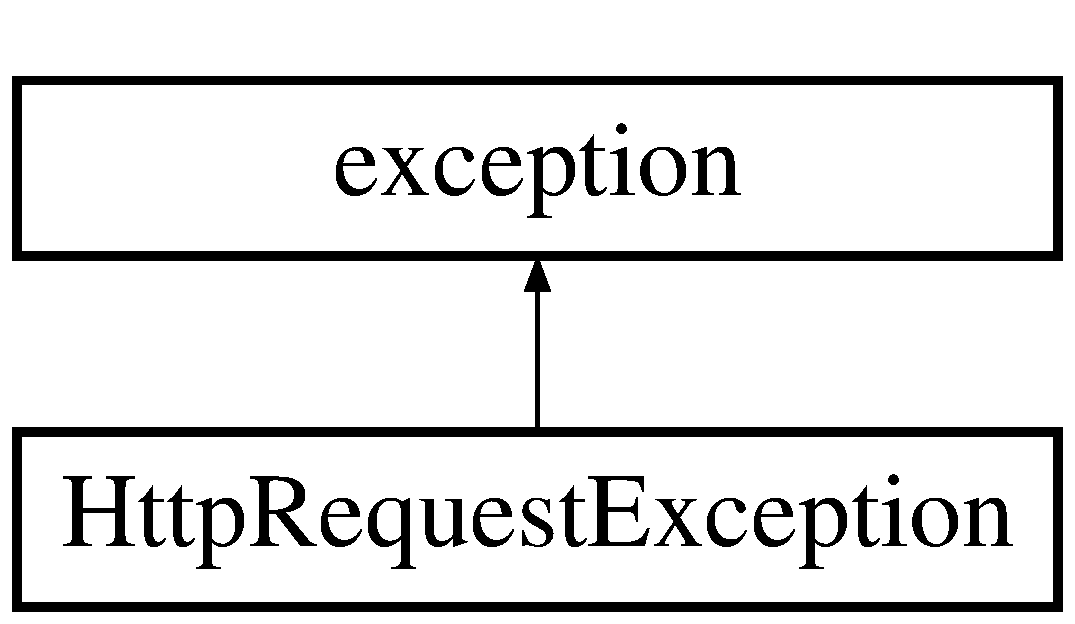
\includegraphics[height=2.000000cm]{structHttpRequestException}
\end{center}
\end{figure}
\subsection*{Public Member Functions}
\begin{DoxyCompactItemize}
\item 
\hypertarget{structHttpRequestException_a8470fe285f8e7f0939b5068546967764}{\hyperlink{structHttpRequestException_a8470fe285f8e7f0939b5068546967764}{Http\-Request\-Exception} (std\-::string msg)}\label{structHttpRequestException_a8470fe285f8e7f0939b5068546967764}

\begin{DoxyCompactList}\small\item\em Create a H\-T\-T\-P \hyperlink{structRequest}{Request} Exception, and store the given error message. \end{DoxyCompactList}\item 
\hypertarget{structHttpRequestException_acf07a2f7382157a27c0c5d2cedb2f2e6}{const char $\ast$ \hyperlink{structHttpRequestException_acf07a2f7382157a27c0c5d2cedb2f2e6}{what} () const   throw ()}\label{structHttpRequestException_acf07a2f7382157a27c0c5d2cedb2f2e6}

\begin{DoxyCompactList}\small\item\em Show the error message in readable format. \end{DoxyCompactList}\end{DoxyCompactItemize}
\subsection*{Public Attributes}
\begin{DoxyCompactItemize}
\item 
\hypertarget{structHttpRequestException_a52a64d4648b543b81050bec3fb039e5f}{std\-::string \hyperlink{structHttpRequestException_a52a64d4648b543b81050bec3fb039e5f}{int\-\_\-msg}}\label{structHttpRequestException_a52a64d4648b543b81050bec3fb039e5f}

\begin{DoxyCompactList}\small\item\em An error message passed on initialization. \end{DoxyCompactList}\end{DoxyCompactItemize}


\subsection{Detailed Description}
An Implementation of std\-::exception that denotes an error during an http operation. 

The documentation for this struct was generated from the following file\-:\begin{DoxyCompactItemize}
\item 
lib/include/factory/http\-\_\-interface.\-h\end{DoxyCompactItemize}

\hypertarget{classHttpServerFactory}{}\section{Http\+Server\+Factory Class Reference}
\label{classHttpServerFactory}\index{Http\+Server\+Factory@{Http\+Server\+Factory}}


The H\+T\+TP Server Service Component Factory.  




{\ttfamily \#include $<$factory\+\_\+http\+\_\+server.\+h$>$}

\subsection*{Public Member Functions}
\begin{DoxyCompactItemize}
\item 
\hyperlink{classHttpServerFactory_aedf936396d36dae5ff39e40f8ffc16b8}{Http\+Server\+Factory} ()\hypertarget{classHttpServerFactory_aedf936396d36dae5ff39e40f8ffc16b8}{}\label{classHttpServerFactory_aedf936396d36dae5ff39e40f8ffc16b8}

\begin{DoxyCompactList}\small\item\em Create a new Service Component Factory. \end{DoxyCompactList}\item 
\hyperlink{classHttpServerFactory_a0db223a7a26a343833ed2b12229189cd}{$\sim$\+Http\+Server\+Factory} ()\hypertarget{classHttpServerFactory_a0db223a7a26a343833ed2b12229189cd}{}\label{classHttpServerFactory_a0db223a7a26a343833ed2b12229189cd}

\begin{DoxyCompactList}\small\item\em Delete a Service Component Factory. \end{DoxyCompactList}\item 
\hyperlink{classHttpServerInterface}{Http\+Server\+Interface} $\ast$ {\bfseries get\+\_\+http\+\_\+server\+\_\+interface} (std\+::string base\+\_\+addr, int base\+\_\+port)\hypertarget{classHttpServerFactory_a423ec1185e8516ca882a61788161f9b4}{}\label{classHttpServerFactory_a423ec1185e8516ca882a61788161f9b4}

\end{DoxyCompactItemize}


\subsection{Detailed Description}
The H\+T\+TP Server Service Component Factory. 

The Service Component Factory tracks the H\+T\+TP Server objects exposed by the framework and passes back instances of interfaces. This allows for the publicly exposed methods to be independent of the implementations. 

The documentation for this class was generated from the following file\+:\begin{DoxyCompactItemize}
\item 
aossl/http/server/include/factory\+\_\+http\+\_\+server.\+h\end{DoxyCompactItemize}

\hypertarget{classHttpServerInterface}{\section{Http\-Server\-Interface Class Reference}
\label{classHttpServerInterface}\index{Http\-Server\-Interface@{Http\-Server\-Interface}}
}


This is a basic H\-T\-T\-P Server that can be used to build a R\-E\-S\-Tful A\-P\-I.  




{\ttfamily \#include $<$http\-\_\-server\-\_\-interface.\-h$>$}

\subsection*{Public Member Functions}
\begin{DoxyCompactItemize}
\item 
\hypertarget{classHttpServerInterface_a6aa54efaf6f176d985c7faa57e1aa7fd}{virtual bool \hyperlink{classHttpServerInterface_a6aa54efaf6f176d985c7faa57e1aa7fd}{bind\-\_\-callback} (std\-::string uri, Callback\-Interface func)=0}\label{classHttpServerInterface_a6aa54efaf6f176d985c7faa57e1aa7fd}

\begin{DoxyCompactList}\small\item\em Bind a callback for a static A\-P\-I Method. \end{DoxyCompactList}\item 
\hypertarget{classHttpServerInterface_a398064a0d7fb0c7e52d94ccfcbb6d89a}{virtual bool \hyperlink{classHttpServerInterface_a398064a0d7fb0c7e52d94ccfcbb6d89a}{bind\-\_\-default\-\_\-callback} (Callback\-Interface func)=0}\label{classHttpServerInterface_a398064a0d7fb0c7e52d94ccfcbb6d89a}

\begin{DoxyCompactList}\small\item\em Bind a callback for a dynamic A\-P\-I Method. \end{DoxyCompactList}\item 
\hypertarget{classHttpServerInterface_a350f4321505079d9c440ce4a4372044f}{virtual void \hyperlink{classHttpServerInterface_a350f4321505079d9c440ce4a4372044f}{recv} ()=0}\label{classHttpServerInterface_a350f4321505079d9c440ce4a4372044f}

\begin{DoxyCompactList}\small\item\em Blocking call for waiting for incoming A\-P\-I Calls. \end{DoxyCompactList}\end{DoxyCompactItemize}


\subsection{Detailed Description}
This is a basic H\-T\-T\-P Server that can be used to build a R\-E\-S\-Tful A\-P\-I. 

The H\-T\-T\-P Server can bind static A\-P\-I methods to individual callbacks, and dynamic A\-P\-I methods can go to a default callback. Used to build R\-E\-S\-Tful A\-P\-I's 

The documentation for this class was generated from the following file\-:\begin{DoxyCompactItemize}
\item 
lib/include/factory/http\-\_\-server\-\_\-interface.\-h\end{DoxyCompactItemize}

\hypertarget{classLoggingCategoryInterface}{}\section{Logging\+Category\+Interface Class Reference}
\label{classLoggingCategoryInterface}\index{Logging\+Category\+Interface@{Logging\+Category\+Interface}}


A Logging Category instantiated on a standard logging instance.  




{\ttfamily \#include $<$logging\+\_\+interface.\+h$>$}

\subsection*{Public Member Functions}
\begin{DoxyCompactItemize}
\item 
virtual void \hyperlink{classLoggingCategoryInterface_aca90c0a8380658a3918ee4c6eb60314b}{debug} (std\+::string msg)=0\hypertarget{classLoggingCategoryInterface_aca90c0a8380658a3918ee4c6eb60314b}{}\label{classLoggingCategoryInterface_aca90c0a8380658a3918ee4c6eb60314b}

\begin{DoxyCompactList}\small\item\em Log at a debug level to the root category. \end{DoxyCompactList}\item 
virtual void \hyperlink{classLoggingCategoryInterface_a377b5248cd5f1c67dc7f13250bf56d78}{error} (std\+::string msg)=0\hypertarget{classLoggingCategoryInterface_a377b5248cd5f1c67dc7f13250bf56d78}{}\label{classLoggingCategoryInterface_a377b5248cd5f1c67dc7f13250bf56d78}

\begin{DoxyCompactList}\small\item\em Log at an error level to the root category. \end{DoxyCompactList}\item 
virtual void \hyperlink{classLoggingCategoryInterface_a2a8bf026f9aeaea95f443744292e237b}{info} (std\+::string msg)=0\hypertarget{classLoggingCategoryInterface_a2a8bf026f9aeaea95f443744292e237b}{}\label{classLoggingCategoryInterface_a2a8bf026f9aeaea95f443744292e237b}

\begin{DoxyCompactList}\small\item\em Log at an info level to the root category. \end{DoxyCompactList}\item 
virtual void \hyperlink{classLoggingCategoryInterface_a6633ea62fbd9850de9f95c42bcb98209}{debug} (const char $\ast$msg)=0\hypertarget{classLoggingCategoryInterface_a6633ea62fbd9850de9f95c42bcb98209}{}\label{classLoggingCategoryInterface_a6633ea62fbd9850de9f95c42bcb98209}

\begin{DoxyCompactList}\small\item\em Log at an debug level to the root category. \end{DoxyCompactList}\item 
virtual void \hyperlink{classLoggingCategoryInterface_a526c3bec470411e17b10a6f38b5477c6}{error} (const char $\ast$msg)=0\hypertarget{classLoggingCategoryInterface_a526c3bec470411e17b10a6f38b5477c6}{}\label{classLoggingCategoryInterface_a526c3bec470411e17b10a6f38b5477c6}

\begin{DoxyCompactList}\small\item\em Log at an error level to the root category. \end{DoxyCompactList}\item 
virtual void \hyperlink{classLoggingCategoryInterface_a5e05b670e8298e0016af09ee5d1c50a6}{info} (const char $\ast$msg)=0\hypertarget{classLoggingCategoryInterface_a5e05b670e8298e0016af09ee5d1c50a6}{}\label{classLoggingCategoryInterface_a5e05b670e8298e0016af09ee5d1c50a6}

\begin{DoxyCompactList}\small\item\em Log at an info level to the root category. \end{DoxyCompactList}\item 
virtual void \hyperlink{classLoggingCategoryInterface_a29536210dbd4617a058cfdad8f8da850}{debug} (int msg)=0\hypertarget{classLoggingCategoryInterface_a29536210dbd4617a058cfdad8f8da850}{}\label{classLoggingCategoryInterface_a29536210dbd4617a058cfdad8f8da850}

\begin{DoxyCompactList}\small\item\em Log at an debug level to the root category. \end{DoxyCompactList}\item 
virtual void \hyperlink{classLoggingCategoryInterface_a5dca5bda32f0f504f2ff2e8a6706f64f}{error} (int msg)=0\hypertarget{classLoggingCategoryInterface_a5dca5bda32f0f504f2ff2e8a6706f64f}{}\label{classLoggingCategoryInterface_a5dca5bda32f0f504f2ff2e8a6706f64f}

\begin{DoxyCompactList}\small\item\em Log at an error level to the root category. \end{DoxyCompactList}\item 
virtual void \hyperlink{classLoggingCategoryInterface_a2c7085aa124ef1e055b43a3c1f4aa866}{info} (int msg)=0\hypertarget{classLoggingCategoryInterface_a2c7085aa124ef1e055b43a3c1f4aa866}{}\label{classLoggingCategoryInterface_a2c7085aa124ef1e055b43a3c1f4aa866}

\begin{DoxyCompactList}\small\item\em Log at an info level to the root category. \end{DoxyCompactList}\item 
virtual void \hyperlink{classLoggingCategoryInterface_aef995a06be8f48121250ceb545ee9ce8}{debug} (float msg)=0\hypertarget{classLoggingCategoryInterface_aef995a06be8f48121250ceb545ee9ce8}{}\label{classLoggingCategoryInterface_aef995a06be8f48121250ceb545ee9ce8}

\begin{DoxyCompactList}\small\item\em Log at an debug level to the root category. \end{DoxyCompactList}\item 
virtual void \hyperlink{classLoggingCategoryInterface_a288016acac317ac5feb149506650431b}{error} (float msg)=0\hypertarget{classLoggingCategoryInterface_a288016acac317ac5feb149506650431b}{}\label{classLoggingCategoryInterface_a288016acac317ac5feb149506650431b}

\begin{DoxyCompactList}\small\item\em Log at an error level to the root category. \end{DoxyCompactList}\item 
virtual void \hyperlink{classLoggingCategoryInterface_abc7a15e2c8befa164be1a0a98df8de26}{info} (float msg)=0\hypertarget{classLoggingCategoryInterface_abc7a15e2c8befa164be1a0a98df8de26}{}\label{classLoggingCategoryInterface_abc7a15e2c8befa164be1a0a98df8de26}

\begin{DoxyCompactList}\small\item\em Log at an info level to the root category. \end{DoxyCompactList}\item 
virtual void \hyperlink{classLoggingCategoryInterface_a12ee058f0418ff5bee7b598df79be600}{debug} (double msg)=0\hypertarget{classLoggingCategoryInterface_a12ee058f0418ff5bee7b598df79be600}{}\label{classLoggingCategoryInterface_a12ee058f0418ff5bee7b598df79be600}

\begin{DoxyCompactList}\small\item\em Log at an debug level to the root category. \end{DoxyCompactList}\item 
virtual void \hyperlink{classLoggingCategoryInterface_a157483fef60e45eb2f6f0d7698d11880}{error} (double msg)=0\hypertarget{classLoggingCategoryInterface_a157483fef60e45eb2f6f0d7698d11880}{}\label{classLoggingCategoryInterface_a157483fef60e45eb2f6f0d7698d11880}

\begin{DoxyCompactList}\small\item\em Log at an error level to the root category. \end{DoxyCompactList}\item 
virtual void \hyperlink{classLoggingCategoryInterface_aa99020d66ab28b686e060112b395b49f}{info} (double msg)=0\hypertarget{classLoggingCategoryInterface_aa99020d66ab28b686e060112b395b49f}{}\label{classLoggingCategoryInterface_aa99020d66ab28b686e060112b395b49f}

\begin{DoxyCompactList}\small\item\em Log at an info level to the root category. \end{DoxyCompactList}\end{DoxyCompactItemize}


\subsection{Detailed Description}
A Logging Category instantiated on a standard logging instance. 

The documentation for this class was generated from the following file\+:\begin{DoxyCompactItemize}
\item 
aossl/logging/include/logging\+\_\+interface.\+h\end{DoxyCompactItemize}

\hypertarget{classLoggingComponentFactory}{}\section{Logging\+Component\+Factory Class Reference}
\label{classLoggingComponentFactory}\index{Logging\+Component\+Factory@{Logging\+Component\+Factory}}


The Logging Service Component Factory.  




{\ttfamily \#include $<$factory\+\_\+logging.\+h$>$}

\subsection*{Public Member Functions}
\begin{DoxyCompactItemize}
\item 
\hyperlink{classLoggingComponentFactory_a0792b093f678c8e6184834a57ee90057}{Logging\+Component\+Factory} ()\hypertarget{classLoggingComponentFactory_a0792b093f678c8e6184834a57ee90057}{}\label{classLoggingComponentFactory_a0792b093f678c8e6184834a57ee90057}

\begin{DoxyCompactList}\small\item\em Create a new Service Component Factory. \end{DoxyCompactList}\item 
\hyperlink{classLoggingComponentFactory_a2fe80510243ff2d5720bf3e4b01d529d}{$\sim$\+Logging\+Component\+Factory} ()\hypertarget{classLoggingComponentFactory_a2fe80510243ff2d5720bf3e4b01d529d}{}\label{classLoggingComponentFactory_a2fe80510243ff2d5720bf3e4b01d529d}

\begin{DoxyCompactList}\small\item\em Delete a Service Component Factory. \end{DoxyCompactList}\item 
\hyperlink{classLoggingInterface}{Logging\+Interface} $\ast$ \hyperlink{classLoggingComponentFactory_a62741318ee4ec84313990989689fc2f0}{get\+\_\+logging\+\_\+interface} (std\+::string init\+File\+Name)\hypertarget{classLoggingComponentFactory_a62741318ee4ec84313990989689fc2f0}{}\label{classLoggingComponentFactory_a62741318ee4ec84313990989689fc2f0}

\begin{DoxyCompactList}\small\item\em Get a Logging Interface instance. \end{DoxyCompactList}\end{DoxyCompactItemize}


\subsection{Detailed Description}
The Logging Service Component Factory. 

The Service Component Factory tracks the Logging objects exposed by the framework and passes back instances of interfaces. This allows for the publicly exposed methods to be independent of the implementations. 

The documentation for this class was generated from the following file\+:\begin{DoxyCompactItemize}
\item 
aossl/logging/include/factory\+\_\+logging.\+h\end{DoxyCompactItemize}

\hypertarget{structLoggingException}{}\section{Logging\+Exception Struct Reference}
\label{structLoggingException}\index{Logging\+Exception@{Logging\+Exception}}


Mongo Exception, used to store errors passed from Mongo.  




{\ttfamily \#include $<$logging\+\_\+interface.\+h$>$}



Inheritance diagram for Logging\+Exception\+:
\nopagebreak
\begin{figure}[H]
\begin{center}
\leavevmode
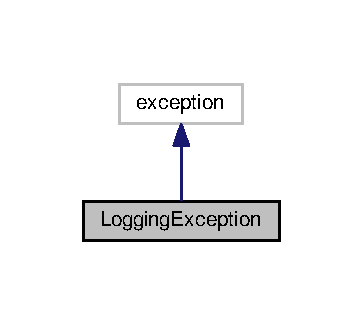
\includegraphics[width=174pt]{structLoggingException__inherit__graph}
\end{center}
\end{figure}


Collaboration diagram for Logging\+Exception\+:
\nopagebreak
\begin{figure}[H]
\begin{center}
\leavevmode
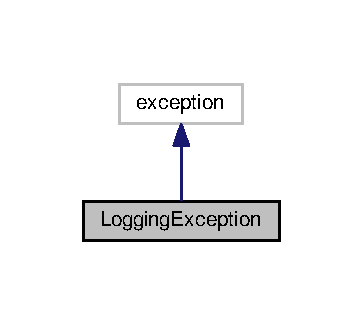
\includegraphics[width=174pt]{structLoggingException__coll__graph}
\end{center}
\end{figure}
\subsection*{Public Member Functions}
\begin{DoxyCompactItemize}
\item 
\hyperlink{structLoggingException_ab82d378b1a05f798ab9b738c79dbec16}{Logging\+Exception} (std\+::string msg)\hypertarget{structLoggingException_ab82d378b1a05f798ab9b738c79dbec16}{}\label{structLoggingException_ab82d378b1a05f798ab9b738c79dbec16}

\begin{DoxyCompactList}\small\item\em Create a Mongo Exception, and store the given error message. \end{DoxyCompactList}\item 
const char $\ast$ \hyperlink{structLoggingException_a2a34c710bcde768940ae6029c2a93f48}{what} () const   throw ()\hypertarget{structLoggingException_a2a34c710bcde768940ae6029c2a93f48}{}\label{structLoggingException_a2a34c710bcde768940ae6029c2a93f48}

\begin{DoxyCompactList}\small\item\em Show the error message in readable format. \end{DoxyCompactList}\end{DoxyCompactItemize}
\subsection*{Public Attributes}
\begin{DoxyCompactItemize}
\item 
std\+::string \hyperlink{structLoggingException_a7b6e62811431fd0f9fc77a70b7e03bb6}{int\+\_\+msg}\hypertarget{structLoggingException_a7b6e62811431fd0f9fc77a70b7e03bb6}{}\label{structLoggingException_a7b6e62811431fd0f9fc77a70b7e03bb6}

\begin{DoxyCompactList}\small\item\em An error message passed on initialization. \end{DoxyCompactList}\item 
const char $\ast$ {\bfseries what\+\_\+str}\hypertarget{structLoggingException_a9734ededaca3a49f66302587e3611c4b}{}\label{structLoggingException_a9734ededaca3a49f66302587e3611c4b}

\end{DoxyCompactItemize}


\subsection{Detailed Description}
Mongo Exception, used to store errors passed from Mongo. 

The documentation for this struct was generated from the following file\+:\begin{DoxyCompactItemize}
\item 
aossl/logging/include/logging\+\_\+interface.\+h\end{DoxyCompactItemize}

\hypertarget{classLoggingInterface}{}\section{Logging\+Interface Class Reference}
\label{classLoggingInterface}\index{Logging\+Interface@{Logging\+Interface}}


An overall logging interface, which can generate logging categories.  




{\ttfamily \#include $<$logging\+\_\+interface.\+h$>$}

\subsection*{Public Member Functions}
\begin{DoxyCompactItemize}
\item 
virtual void \hyperlink{classLoggingInterface_a94e666bf17b42a65c03aff86cbe04978}{debug} (std\+::string msg)=0\hypertarget{classLoggingInterface_a94e666bf17b42a65c03aff86cbe04978}{}\label{classLoggingInterface_a94e666bf17b42a65c03aff86cbe04978}

\begin{DoxyCompactList}\small\item\em Log at a debug level to the root category. \end{DoxyCompactList}\item 
virtual void \hyperlink{classLoggingInterface_a86ba6616c2163d8cb49bed70def8b862}{error} (std\+::string msg)=0\hypertarget{classLoggingInterface_a86ba6616c2163d8cb49bed70def8b862}{}\label{classLoggingInterface_a86ba6616c2163d8cb49bed70def8b862}

\begin{DoxyCompactList}\small\item\em Log at an error level to the root category. \end{DoxyCompactList}\item 
virtual void \hyperlink{classLoggingInterface_a5d994f7cfafe81171954409df64d77ce}{info} (std\+::string msg)=0\hypertarget{classLoggingInterface_a5d994f7cfafe81171954409df64d77ce}{}\label{classLoggingInterface_a5d994f7cfafe81171954409df64d77ce}

\begin{DoxyCompactList}\small\item\em Log at an info level to the root category. \end{DoxyCompactList}\item 
virtual void \hyperlink{classLoggingInterface_a82c2727fb66531d5eec19e39bed79671}{debug} (const char $\ast$msg)=0\hypertarget{classLoggingInterface_a82c2727fb66531d5eec19e39bed79671}{}\label{classLoggingInterface_a82c2727fb66531d5eec19e39bed79671}

\begin{DoxyCompactList}\small\item\em Log at an debug level to the root category. \end{DoxyCompactList}\item 
virtual void \hyperlink{classLoggingInterface_a1cea9e37dae316f39e171654e5e0dc0f}{error} (const char $\ast$msg)=0\hypertarget{classLoggingInterface_a1cea9e37dae316f39e171654e5e0dc0f}{}\label{classLoggingInterface_a1cea9e37dae316f39e171654e5e0dc0f}

\begin{DoxyCompactList}\small\item\em Log at an error level to the root category. \end{DoxyCompactList}\item 
virtual void \hyperlink{classLoggingInterface_a7aed25910dd1cdebe3906b4b33d75a80}{info} (const char $\ast$msg)=0\hypertarget{classLoggingInterface_a7aed25910dd1cdebe3906b4b33d75a80}{}\label{classLoggingInterface_a7aed25910dd1cdebe3906b4b33d75a80}

\begin{DoxyCompactList}\small\item\em Log at an info level to the root category. \end{DoxyCompactList}\item 
virtual void \hyperlink{classLoggingInterface_a66b4e3f845501917df8975e95157f436}{debug} (int msg)=0\hypertarget{classLoggingInterface_a66b4e3f845501917df8975e95157f436}{}\label{classLoggingInterface_a66b4e3f845501917df8975e95157f436}

\begin{DoxyCompactList}\small\item\em Log at an debug level to the root category. \end{DoxyCompactList}\item 
virtual void \hyperlink{classLoggingInterface_a85fa61f75508d25d846f7ac39790c457}{error} (int msg)=0\hypertarget{classLoggingInterface_a85fa61f75508d25d846f7ac39790c457}{}\label{classLoggingInterface_a85fa61f75508d25d846f7ac39790c457}

\begin{DoxyCompactList}\small\item\em Log at an error level to the root category. \end{DoxyCompactList}\item 
virtual void \hyperlink{classLoggingInterface_a724cb769b7233a783956e9fa41ff7291}{info} (int msg)=0\hypertarget{classLoggingInterface_a724cb769b7233a783956e9fa41ff7291}{}\label{classLoggingInterface_a724cb769b7233a783956e9fa41ff7291}

\begin{DoxyCompactList}\small\item\em Log at an info level to the root category. \end{DoxyCompactList}\item 
virtual void \hyperlink{classLoggingInterface_a301a0e53971f7fabd6f296722738aeff}{debug} (float msg)=0\hypertarget{classLoggingInterface_a301a0e53971f7fabd6f296722738aeff}{}\label{classLoggingInterface_a301a0e53971f7fabd6f296722738aeff}

\begin{DoxyCompactList}\small\item\em Log at an debug level to the root category. \end{DoxyCompactList}\item 
virtual void \hyperlink{classLoggingInterface_adab4f9849012eca577d04981e185d08c}{error} (float msg)=0\hypertarget{classLoggingInterface_adab4f9849012eca577d04981e185d08c}{}\label{classLoggingInterface_adab4f9849012eca577d04981e185d08c}

\begin{DoxyCompactList}\small\item\em Log at an error level to the root category. \end{DoxyCompactList}\item 
virtual void \hyperlink{classLoggingInterface_aebe8b51717ca65efb39cea955aa24e73}{info} (float msg)=0\hypertarget{classLoggingInterface_aebe8b51717ca65efb39cea955aa24e73}{}\label{classLoggingInterface_aebe8b51717ca65efb39cea955aa24e73}

\begin{DoxyCompactList}\small\item\em Log at an info level to the root category. \end{DoxyCompactList}\item 
virtual void \hyperlink{classLoggingInterface_afbb073b280b346f52b1b26be9aad9c9c}{debug} (double msg)=0\hypertarget{classLoggingInterface_afbb073b280b346f52b1b26be9aad9c9c}{}\label{classLoggingInterface_afbb073b280b346f52b1b26be9aad9c9c}

\begin{DoxyCompactList}\small\item\em Log at an debug level to the root category. \end{DoxyCompactList}\item 
virtual void \hyperlink{classLoggingInterface_ad7e7ef57f8aba34cb9df9788b52faae7}{error} (double msg)=0\hypertarget{classLoggingInterface_ad7e7ef57f8aba34cb9df9788b52faae7}{}\label{classLoggingInterface_ad7e7ef57f8aba34cb9df9788b52faae7}

\begin{DoxyCompactList}\small\item\em Log at an error level to the root category. \end{DoxyCompactList}\item 
virtual void \hyperlink{classLoggingInterface_a6e196d311e2b078071a3a4a8337a6264}{info} (double msg)=0\hypertarget{classLoggingInterface_a6e196d311e2b078071a3a4a8337a6264}{}\label{classLoggingInterface_a6e196d311e2b078071a3a4a8337a6264}

\begin{DoxyCompactList}\small\item\em Log at an info level to the root category. \end{DoxyCompactList}\item 
virtual \hyperlink{classLoggingCategoryInterface}{Logging\+Category\+Interface} $\ast$ \hyperlink{classLoggingInterface_add380ece858220c46aeb38ce1531a6c7}{get\+\_\+category} (std\+::string name)=0\hypertarget{classLoggingInterface_add380ece858220c46aeb38ce1531a6c7}{}\label{classLoggingInterface_add380ece858220c46aeb38ce1531a6c7}

\begin{DoxyCompactList}\small\item\em Pull down different categories by name. \end{DoxyCompactList}\end{DoxyCompactItemize}


\subsection{Detailed Description}
An overall logging interface, which can generate logging categories. 

The documentation for this class was generated from the following file\+:\begin{DoxyCompactItemize}
\item 
aossl/logging/include/logging\+\_\+interface.\+h\end{DoxyCompactItemize}

\hypertarget{classMongoComponentFactory}{}\section{Mongo\+Component\+Factory Class Reference}
\label{classMongoComponentFactory}\index{Mongo\+Component\+Factory@{Mongo\+Component\+Factory}}


The Mongo Service Component Factory.  




{\ttfamily \#include $<$factory\+\_\+mongo.\+h$>$}

\subsection*{Public Member Functions}
\begin{DoxyCompactItemize}
\item 
\hyperlink{classMongoComponentFactory_ad98b89af9397105639e36f985d368f21}{Mongo\+Component\+Factory} ()\hypertarget{classMongoComponentFactory_ad98b89af9397105639e36f985d368f21}{}\label{classMongoComponentFactory_ad98b89af9397105639e36f985d368f21}

\begin{DoxyCompactList}\small\item\em Create a new Service Component Factory. \end{DoxyCompactList}\item 
\hyperlink{classMongoComponentFactory_a861f52374272dc439fcee8d3de2e09ee}{$\sim$\+Mongo\+Component\+Factory} ()\hypertarget{classMongoComponentFactory_a861f52374272dc439fcee8d3de2e09ee}{}\label{classMongoComponentFactory_a861f52374272dc439fcee8d3de2e09ee}

\begin{DoxyCompactList}\small\item\em Delete a Service Component Factory. \end{DoxyCompactList}\item 
\hyperlink{classMongoInterface}{Mongo\+Interface} $\ast$ \hyperlink{classMongoComponentFactory_a67388e5603e265ddfe0246d6726baf24}{get\+\_\+mongo\+\_\+interface} (const char $\ast$url, const char $\ast$db, const char $\ast$collection\+\_\+name)\hypertarget{classMongoComponentFactory_a67388e5603e265ddfe0246d6726baf24}{}\label{classMongoComponentFactory_a67388e5603e265ddfe0246d6726baf24}

\begin{DoxyCompactList}\small\item\em Get a Mongo Interface instance. \end{DoxyCompactList}\item 
\hyperlink{classMongoInterface}{Mongo\+Interface} $\ast$ \hyperlink{classMongoComponentFactory_a95778473e6c83acae99e3c27155ab5fd}{get\+\_\+mongo\+\_\+interface} (std\+::string url, std\+::string db, std\+::string collection\+\_\+name)\hypertarget{classMongoComponentFactory_a95778473e6c83acae99e3c27155ab5fd}{}\label{classMongoComponentFactory_a95778473e6c83acae99e3c27155ab5fd}

\begin{DoxyCompactList}\small\item\em Get a Mongo Interface instance. \end{DoxyCompactList}\item 
\hyperlink{classMongoInterface}{Mongo\+Interface} $\ast$ \hyperlink{classMongoComponentFactory_ae76578bb9a27d48d826840dc3be913d4}{get\+\_\+mongo\+\_\+interface} (const char $\ast$url, const char $\ast$db)\hypertarget{classMongoComponentFactory_ae76578bb9a27d48d826840dc3be913d4}{}\label{classMongoComponentFactory_ae76578bb9a27d48d826840dc3be913d4}

\begin{DoxyCompactList}\small\item\em Get a Mongo Interface instance. \end{DoxyCompactList}\item 
\hyperlink{classMongoInterface}{Mongo\+Interface} $\ast$ \hyperlink{classMongoComponentFactory_addd2a8eabc1d264f911027e1bd64aac7}{get\+\_\+mongo\+\_\+interface} (std\+::string url, std\+::string db)\hypertarget{classMongoComponentFactory_addd2a8eabc1d264f911027e1bd64aac7}{}\label{classMongoComponentFactory_addd2a8eabc1d264f911027e1bd64aac7}

\begin{DoxyCompactList}\small\item\em Get a Mongo Interface instance. \end{DoxyCompactList}\item 
\hyperlink{classMongoInterface}{Mongo\+Interface} $\ast$ \hyperlink{classMongoComponentFactory_a5e4c960eda23c22134685640a3ced24c}{get\+\_\+mongo\+\_\+interface} (const char $\ast$url, const char $\ast$db, const char $\ast$collection\+\_\+name, int pool\+\_\+size)\hypertarget{classMongoComponentFactory_a5e4c960eda23c22134685640a3ced24c}{}\label{classMongoComponentFactory_a5e4c960eda23c22134685640a3ced24c}

\begin{DoxyCompactList}\small\item\em Get a Mongo Interface instance. \end{DoxyCompactList}\item 
\hyperlink{classMongoInterface}{Mongo\+Interface} $\ast$ \hyperlink{classMongoComponentFactory_ab2b7e0247e44b133dec4ab391d2b76de}{get\+\_\+mongo\+\_\+interface} (std\+::string url, std\+::string db, std\+::string collection\+\_\+name, int pool\+\_\+size)\hypertarget{classMongoComponentFactory_ab2b7e0247e44b133dec4ab391d2b76de}{}\label{classMongoComponentFactory_ab2b7e0247e44b133dec4ab391d2b76de}

\begin{DoxyCompactList}\small\item\em Get a Mongo Interface instance. \end{DoxyCompactList}\item 
\hyperlink{classMongoInterface}{Mongo\+Interface} $\ast$ \hyperlink{classMongoComponentFactory_a16b0cd08ee59bfb951b89ddd0a47f18e}{get\+\_\+mongo\+\_\+interface} (const char $\ast$url, const char $\ast$db, int pool\+\_\+size)\hypertarget{classMongoComponentFactory_a16b0cd08ee59bfb951b89ddd0a47f18e}{}\label{classMongoComponentFactory_a16b0cd08ee59bfb951b89ddd0a47f18e}

\begin{DoxyCompactList}\small\item\em Get a Mongo Interface instance. \end{DoxyCompactList}\item 
\hyperlink{classMongoInterface}{Mongo\+Interface} $\ast$ \hyperlink{classMongoComponentFactory_a22622652c551250f1dbefd4a713960cf}{get\+\_\+mongo\+\_\+interface} (std\+::string url, std\+::string db, int pool\+\_\+size)\hypertarget{classMongoComponentFactory_a22622652c551250f1dbefd4a713960cf}{}\label{classMongoComponentFactory_a22622652c551250f1dbefd4a713960cf}

\begin{DoxyCompactList}\small\item\em Get a Mongo Interface instance. \end{DoxyCompactList}\end{DoxyCompactItemize}


\subsection{Detailed Description}
The Mongo Service Component Factory. 

The Service Component Factory tracks the Mongo objects exposed by the framework and passes back instances of interfaces. This allows for the publicly exposed methods to be independent of the implementations. 

The documentation for this class was generated from the following file\+:\begin{DoxyCompactItemize}
\item 
aossl/mongo/include/factory\+\_\+mongo.\+h\end{DoxyCompactItemize}

\hypertarget{structMongoException}{\section{Mongo\-Exception Struct Reference}
\label{structMongoException}\index{Mongo\-Exception@{Mongo\-Exception}}
}
Inheritance diagram for Mongo\-Exception\-:\begin{figure}[H]
\begin{center}
\leavevmode
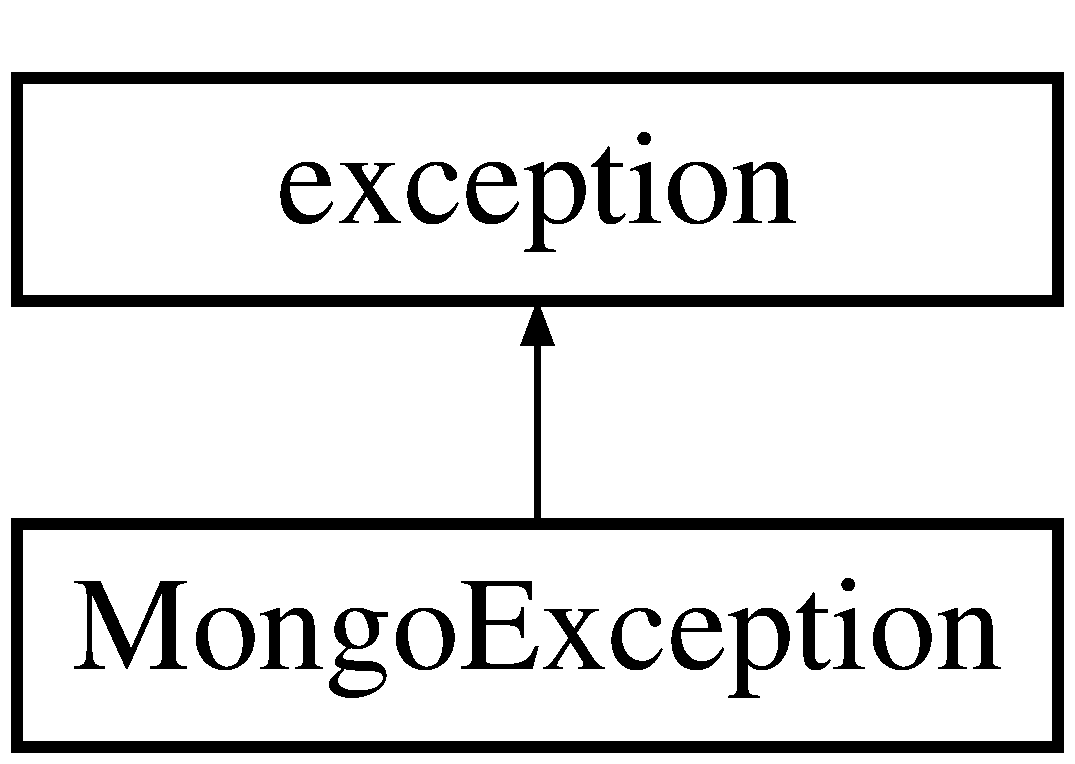
\includegraphics[height=2.000000cm]{structMongoException}
\end{center}
\end{figure}
\subsection*{Public Member Functions}
\begin{DoxyCompactItemize}
\item 
\hypertarget{structMongoException_addaa545189ab30bcc6a0e957514253fa}{\hyperlink{structMongoException_addaa545189ab30bcc6a0e957514253fa}{Mongo\-Exception} (std\-::string msg)}\label{structMongoException_addaa545189ab30bcc6a0e957514253fa}

\begin{DoxyCompactList}\small\item\em Create a Mongo Exception, and store the given error message. \end{DoxyCompactList}\item 
\hypertarget{structMongoException_a5202b0dfc3d8a554d9f36e4b1c31c2a3}{const char $\ast$ \hyperlink{structMongoException_a5202b0dfc3d8a554d9f36e4b1c31c2a3}{what} () const   throw ()}\label{structMongoException_a5202b0dfc3d8a554d9f36e4b1c31c2a3}

\begin{DoxyCompactList}\small\item\em Show the error message in readable format. \end{DoxyCompactList}\end{DoxyCompactItemize}
\subsection*{Public Attributes}
\begin{DoxyCompactItemize}
\item 
\hypertarget{structMongoException_ae5a0824b7a469b66dcc3947704310e4c}{std\-::string \hyperlink{structMongoException_ae5a0824b7a469b66dcc3947704310e4c}{int\-\_\-msg}}\label{structMongoException_ae5a0824b7a469b66dcc3947704310e4c}

\begin{DoxyCompactList}\small\item\em An error message passed on initialization. \end{DoxyCompactList}\end{DoxyCompactItemize}


The documentation for this struct was generated from the following file\-:\begin{DoxyCompactItemize}
\item 
lib/include/factory/mongo\-\_\-interface.\-h\end{DoxyCompactItemize}

\hypertarget{classMongoInterface}{}\section{Mongo\+Interface Class Reference}
\label{classMongoInterface}\index{Mongo\+Interface@{Mongo\+Interface}}
\subsection*{Public Member Functions}
\begin{DoxyCompactItemize}
\item 
virtual \hyperlink{classMongoResponseInterface}{Mongo\+Response\+Interface} $\ast$ \hyperlink{classMongoInterface_a40a5973d65dd15c46df9f6c06fbb464a}{create\+\_\+document} (const char $\ast$doc, const char $\ast$collection\+\_\+name)=0\hypertarget{classMongoInterface_a40a5973d65dd15c46df9f6c06fbb464a}{}\label{classMongoInterface_a40a5973d65dd15c46df9f6c06fbb464a}

\begin{DoxyCompactList}\small\item\em Create J\+S\+ON Document, returns the document key. \end{DoxyCompactList}\item 
virtual \hyperlink{classMongoResponseInterface}{Mongo\+Response\+Interface} $\ast$ \hyperlink{classMongoInterface_af621e8af8a4205e1cf06d1964ba36843}{create\+\_\+document} (const char $\ast$doc)=0\hypertarget{classMongoInterface_af621e8af8a4205e1cf06d1964ba36843}{}\label{classMongoInterface_af621e8af8a4205e1cf06d1964ba36843}

\begin{DoxyCompactList}\small\item\em Create J\+S\+ON Document, returns the document key. \end{DoxyCompactList}\item 
virtual \hyperlink{classMongoResponseInterface}{Mongo\+Response\+Interface} $\ast$ \hyperlink{classMongoInterface_aaa549157c25eef7e9ed21b143c28bb64}{create\+\_\+document} (std\+::string doc)=0\hypertarget{classMongoInterface_aaa549157c25eef7e9ed21b143c28bb64}{}\label{classMongoInterface_aaa549157c25eef7e9ed21b143c28bb64}

\begin{DoxyCompactList}\small\item\em Create J\+S\+ON Document, returns the document key. \end{DoxyCompactList}\item 
virtual \hyperlink{classMongoResponseInterface}{Mongo\+Response\+Interface} $\ast$ \hyperlink{classMongoInterface_a5870d9a0cb64044d195893cc4d59801f}{create\+\_\+document} (std\+::string doc, std\+::string collection\+\_\+name)=0\hypertarget{classMongoInterface_a5870d9a0cb64044d195893cc4d59801f}{}\label{classMongoInterface_a5870d9a0cb64044d195893cc4d59801f}

\begin{DoxyCompactList}\small\item\em Create J\+S\+ON Document, returns the document key. \end{DoxyCompactList}\item 
virtual void \hyperlink{classMongoInterface_a9153c6d0c292aa76e51bf65c41d51f8d}{delete\+\_\+document} (const char $\ast$key)=0\hypertarget{classMongoInterface_a9153c6d0c292aa76e51bf65c41d51f8d}{}\label{classMongoInterface_a9153c6d0c292aa76e51bf65c41d51f8d}

\begin{DoxyCompactList}\small\item\em Delete a J\+S\+ON Document, returns true if successful. \end{DoxyCompactList}\item 
virtual void \hyperlink{classMongoInterface_a9e15069c0c05f9aa89918fd39c0e7a94}{delete\+\_\+document} (std\+::string key)=0\hypertarget{classMongoInterface_a9e15069c0c05f9aa89918fd39c0e7a94}{}\label{classMongoInterface_a9e15069c0c05f9aa89918fd39c0e7a94}

\begin{DoxyCompactList}\small\item\em Delete a J\+S\+ON Document, returns true if successful. \end{DoxyCompactList}\item 
virtual void \hyperlink{classMongoInterface_abc9fd636d41e508ede790754e4dbab86}{delete\+\_\+document} (const char $\ast$key, const char $\ast$collection\+\_\+name)=0\hypertarget{classMongoInterface_abc9fd636d41e508ede790754e4dbab86}{}\label{classMongoInterface_abc9fd636d41e508ede790754e4dbab86}

\begin{DoxyCompactList}\small\item\em Delete a J\+S\+ON Document, returns true if successful. \end{DoxyCompactList}\item 
virtual void \hyperlink{classMongoInterface_ae00271d50df56c537627031c0ecef0d6}{delete\+\_\+document} (std\+::string key, std\+::string collection\+\_\+name)=0\hypertarget{classMongoInterface_ae00271d50df56c537627031c0ecef0d6}{}\label{classMongoInterface_ae00271d50df56c537627031c0ecef0d6}

\begin{DoxyCompactList}\small\item\em Delete a J\+S\+ON Document, returns true if successful. \end{DoxyCompactList}\item 
virtual \hyperlink{classMongoResponseInterface}{Mongo\+Response\+Interface} $\ast$ \hyperlink{classMongoInterface_acc6a2b3cc3cf9dcbc0cdb44ddbd14674}{load\+\_\+document} (const char $\ast$key)=0\hypertarget{classMongoInterface_acc6a2b3cc3cf9dcbc0cdb44ddbd14674}{}\label{classMongoInterface_acc6a2b3cc3cf9dcbc0cdb44ddbd14674}

\begin{DoxyCompactList}\small\item\em Retrieve a J\+S\+ON Document and return it in a std\+::string. \end{DoxyCompactList}\item 
virtual \hyperlink{classMongoResponseInterface}{Mongo\+Response\+Interface} $\ast$ \hyperlink{classMongoInterface_a19e569ead19f32799fa49805a6345551}{load\+\_\+document} (std\+::string key)=0\hypertarget{classMongoInterface_a19e569ead19f32799fa49805a6345551}{}\label{classMongoInterface_a19e569ead19f32799fa49805a6345551}

\begin{DoxyCompactList}\small\item\em Retrieve a J\+S\+ON Document and return it in a std\+::string. \end{DoxyCompactList}\item 
virtual \hyperlink{classMongoResponseInterface}{Mongo\+Response\+Interface} $\ast$ \hyperlink{classMongoInterface_abb8bf5ca5eed49b76fd91adcf3a8dfc8}{load\+\_\+document} (const char $\ast$key, const char $\ast$collection\+\_\+name)=0\hypertarget{classMongoInterface_abb8bf5ca5eed49b76fd91adcf3a8dfc8}{}\label{classMongoInterface_abb8bf5ca5eed49b76fd91adcf3a8dfc8}

\begin{DoxyCompactList}\small\item\em Retrieve a J\+S\+ON Document and return it in a std\+::string. \end{DoxyCompactList}\item 
virtual \hyperlink{classMongoResponseInterface}{Mongo\+Response\+Interface} $\ast$ \hyperlink{classMongoInterface_a7635ac63b0968306687632d037df5d4a}{load\+\_\+document} (std\+::string key, std\+::string collection\+\_\+name)=0\hypertarget{classMongoInterface_a7635ac63b0968306687632d037df5d4a}{}\label{classMongoInterface_a7635ac63b0968306687632d037df5d4a}

\begin{DoxyCompactList}\small\item\em Retrieve a J\+S\+ON Document and return it in a std\+::string. \end{DoxyCompactList}\item 
virtual void \hyperlink{classMongoInterface_a05885b7361096a03b623da8c7b48e461}{save\+\_\+document} (const char $\ast$doc, const char $\ast$key)=0\hypertarget{classMongoInterface_a05885b7361096a03b623da8c7b48e461}{}\label{classMongoInterface_a05885b7361096a03b623da8c7b48e461}

\begin{DoxyCompactList}\small\item\em Update an existing document, returns true if successful. \end{DoxyCompactList}\item 
virtual void \hyperlink{classMongoInterface_a35888cb594d1f46d52147649786e948f}{save\+\_\+document} (std\+::string doc, std\+::string key)=0\hypertarget{classMongoInterface_a35888cb594d1f46d52147649786e948f}{}\label{classMongoInterface_a35888cb594d1f46d52147649786e948f}

\begin{DoxyCompactList}\small\item\em Update an existing document, returns true if successful. \end{DoxyCompactList}\item 
virtual void \hyperlink{classMongoInterface_a4d2c3e6a8fb172f8d07fc3dd710053ae}{save\+\_\+document} (const char $\ast$doc, const char $\ast$key, const char $\ast$collection\+\_\+name)=0\hypertarget{classMongoInterface_a4d2c3e6a8fb172f8d07fc3dd710053ae}{}\label{classMongoInterface_a4d2c3e6a8fb172f8d07fc3dd710053ae}

\begin{DoxyCompactList}\small\item\em Update an existing document, returns true if successful. \end{DoxyCompactList}\item 
virtual void \hyperlink{classMongoInterface_a14f3c2a76a495777a1f48ed155831134}{save\+\_\+document} (std\+::string doc, std\+::string key, std\+::string collection\+\_\+name)=0\hypertarget{classMongoInterface_a14f3c2a76a495777a1f48ed155831134}{}\label{classMongoInterface_a14f3c2a76a495777a1f48ed155831134}

\begin{DoxyCompactList}\small\item\em Update an existing document, returns true if successful. \end{DoxyCompactList}\item 
virtual \hyperlink{classMongoIteratorInterface}{Mongo\+Iterator\+Interface} $\ast$ \hyperlink{classMongoInterface_a15ceb9bc80b43bc09afd0d5e32cea4f7}{query} (const char $\ast$query\+\_\+str, const char $\ast$opts\+\_\+str)=0
\begin{DoxyCompactList}\small\item\em Queries. \end{DoxyCompactList}\item 
virtual \hyperlink{classMongoIteratorInterface}{Mongo\+Iterator\+Interface} $\ast$ \hyperlink{classMongoInterface_a6f5d8758fe477e997df995028afe82a4}{query} (std\+::string query\+\_\+str, std\+::string opts\+\_\+str)=0
\begin{DoxyCompactList}\small\item\em Queries. \end{DoxyCompactList}\item 
virtual \hyperlink{classMongoIteratorInterface}{Mongo\+Iterator\+Interface} $\ast$ \hyperlink{classMongoInterface_ab4aa9b1a60d96ffcf787114fc2d436b0}{query} (const char $\ast$query\+\_\+str, const char $\ast$opts\+\_\+str, const char $\ast$collection\+\_\+name)=0
\begin{DoxyCompactList}\small\item\em Queries. \end{DoxyCompactList}\item 
virtual \hyperlink{classMongoIteratorInterface}{Mongo\+Iterator\+Interface} $\ast$ \hyperlink{classMongoInterface_a37fd750f45fc0a9b7360c3ad433c1747}{query} (std\+::string query\+\_\+str, std\+::string opts\+\_\+str, std\+::string collection\+\_\+name)=0
\begin{DoxyCompactList}\small\item\em Queries. \end{DoxyCompactList}\item 
virtual \hyperlink{classMongoIteratorInterface}{Mongo\+Iterator\+Interface} $\ast$ \hyperlink{classMongoInterface_a53f62c62e8a54abcb6ead11e544b51d0}{query} (const char $\ast$query\+\_\+str)=0
\begin{DoxyCompactList}\small\item\em Queries. \end{DoxyCompactList}\item 
virtual \hyperlink{classMongoIteratorInterface}{Mongo\+Iterator\+Interface} $\ast$ \hyperlink{classMongoInterface_afbfd334e99d9c1861ea9c4623b326e48}{query} (std\+::string query\+\_\+str)=0
\begin{DoxyCompactList}\small\item\em Queries. \end{DoxyCompactList}\end{DoxyCompactItemize}


\subsection{Member Function Documentation}
\index{Mongo\+Interface@{Mongo\+Interface}!query@{query}}
\index{query@{query}!Mongo\+Interface@{Mongo\+Interface}}
\subsubsection[{\texorpdfstring{query(const char $\ast$query\+\_\+str, const char $\ast$opts\+\_\+str)=0}{query(const char *query_str, const char *opts_str)=0}}]{\setlength{\rightskip}{0pt plus 5cm}virtual {\bf Mongo\+Iterator\+Interface}$\ast$ Mongo\+Interface\+::query (
\begin{DoxyParamCaption}
\item[{const char $\ast$}]{query\+\_\+str, }
\item[{const char $\ast$}]{opts\+\_\+str}
\end{DoxyParamCaption}
)\hspace{0.3cm}{\ttfamily [pure virtual]}}\hypertarget{classMongoInterface_a15ceb9bc80b43bc09afd0d5e32cea4f7}{}\label{classMongoInterface_a15ceb9bc80b43bc09afd0d5e32cea4f7}


Queries. 

Accept the query and query options in J\+S\+ON format. Return an iterator which can be used to access query results \index{Mongo\+Interface@{Mongo\+Interface}!query@{query}}
\index{query@{query}!Mongo\+Interface@{Mongo\+Interface}}
\subsubsection[{\texorpdfstring{query(std\+::string query\+\_\+str, std\+::string opts\+\_\+str)=0}{query(std::string query_str, std::string opts_str)=0}}]{\setlength{\rightskip}{0pt plus 5cm}virtual {\bf Mongo\+Iterator\+Interface}$\ast$ Mongo\+Interface\+::query (
\begin{DoxyParamCaption}
\item[{std\+::string}]{query\+\_\+str, }
\item[{std\+::string}]{opts\+\_\+str}
\end{DoxyParamCaption}
)\hspace{0.3cm}{\ttfamily [pure virtual]}}\hypertarget{classMongoInterface_a6f5d8758fe477e997df995028afe82a4}{}\label{classMongoInterface_a6f5d8758fe477e997df995028afe82a4}


Queries. 

Accept the query and query options in J\+S\+ON format. Return an iterator which can be used to access query results \index{Mongo\+Interface@{Mongo\+Interface}!query@{query}}
\index{query@{query}!Mongo\+Interface@{Mongo\+Interface}}
\subsubsection[{\texorpdfstring{query(const char $\ast$query\+\_\+str, const char $\ast$opts\+\_\+str, const char $\ast$collection\+\_\+name)=0}{query(const char *query_str, const char *opts_str, const char *collection_name)=0}}]{\setlength{\rightskip}{0pt plus 5cm}virtual {\bf Mongo\+Iterator\+Interface}$\ast$ Mongo\+Interface\+::query (
\begin{DoxyParamCaption}
\item[{const char $\ast$}]{query\+\_\+str, }
\item[{const char $\ast$}]{opts\+\_\+str, }
\item[{const char $\ast$}]{collection\+\_\+name}
\end{DoxyParamCaption}
)\hspace{0.3cm}{\ttfamily [pure virtual]}}\hypertarget{classMongoInterface_ab4aa9b1a60d96ffcf787114fc2d436b0}{}\label{classMongoInterface_ab4aa9b1a60d96ffcf787114fc2d436b0}


Queries. 

Accept the query and query options in J\+S\+ON format. Return an iterator which can be used to access query results \index{Mongo\+Interface@{Mongo\+Interface}!query@{query}}
\index{query@{query}!Mongo\+Interface@{Mongo\+Interface}}
\subsubsection[{\texorpdfstring{query(std\+::string query\+\_\+str, std\+::string opts\+\_\+str, std\+::string collection\+\_\+name)=0}{query(std::string query_str, std::string opts_str, std::string collection_name)=0}}]{\setlength{\rightskip}{0pt plus 5cm}virtual {\bf Mongo\+Iterator\+Interface}$\ast$ Mongo\+Interface\+::query (
\begin{DoxyParamCaption}
\item[{std\+::string}]{query\+\_\+str, }
\item[{std\+::string}]{opts\+\_\+str, }
\item[{std\+::string}]{collection\+\_\+name}
\end{DoxyParamCaption}
)\hspace{0.3cm}{\ttfamily [pure virtual]}}\hypertarget{classMongoInterface_a37fd750f45fc0a9b7360c3ad433c1747}{}\label{classMongoInterface_a37fd750f45fc0a9b7360c3ad433c1747}


Queries. 

Accept the query and query options in J\+S\+ON format. Return an iterator which can be used to access query results \index{Mongo\+Interface@{Mongo\+Interface}!query@{query}}
\index{query@{query}!Mongo\+Interface@{Mongo\+Interface}}
\subsubsection[{\texorpdfstring{query(const char $\ast$query\+\_\+str)=0}{query(const char *query_str)=0}}]{\setlength{\rightskip}{0pt plus 5cm}virtual {\bf Mongo\+Iterator\+Interface}$\ast$ Mongo\+Interface\+::query (
\begin{DoxyParamCaption}
\item[{const char $\ast$}]{query\+\_\+str}
\end{DoxyParamCaption}
)\hspace{0.3cm}{\ttfamily [pure virtual]}}\hypertarget{classMongoInterface_a53f62c62e8a54abcb6ead11e544b51d0}{}\label{classMongoInterface_a53f62c62e8a54abcb6ead11e544b51d0}


Queries. 

Accept the query in J\+S\+ON format. Return an iterator which can be used to access query results \index{Mongo\+Interface@{Mongo\+Interface}!query@{query}}
\index{query@{query}!Mongo\+Interface@{Mongo\+Interface}}
\subsubsection[{\texorpdfstring{query(std\+::string query\+\_\+str)=0}{query(std::string query_str)=0}}]{\setlength{\rightskip}{0pt plus 5cm}virtual {\bf Mongo\+Iterator\+Interface}$\ast$ Mongo\+Interface\+::query (
\begin{DoxyParamCaption}
\item[{std\+::string}]{query\+\_\+str}
\end{DoxyParamCaption}
)\hspace{0.3cm}{\ttfamily [pure virtual]}}\hypertarget{classMongoInterface_afbfd334e99d9c1861ea9c4623b326e48}{}\label{classMongoInterface_afbfd334e99d9c1861ea9c4623b326e48}


Queries. 

Accept the query in J\+S\+ON format. Return an iterator which can be used to access query results 

The documentation for this class was generated from the following file\+:\begin{DoxyCompactItemize}
\item 
aossl/mongo/include/mongo\+\_\+interface.\+h\end{DoxyCompactItemize}

\hypertarget{classMongoIteratorInterface}{}\section{Mongo\+Iterator\+Interface Class Reference}
\label{classMongoIteratorInterface}\index{Mongo\+Iterator\+Interface@{Mongo\+Iterator\+Interface}}


Returned from Queries in order to iterate over results.  




{\ttfamily \#include $<$mongo\+\_\+interface.\+h$>$}

\subsection*{Public Member Functions}
\begin{DoxyCompactItemize}
\item 
virtual \hyperlink{classMongoResponseInterface}{Mongo\+Response\+Interface} $\ast$ \hyperlink{classMongoIteratorInterface_a17596bbbf5678973d0c07ac82cb0ccaa}{next} ()=0
\begin{DoxyCompactList}\small\item\em Get the next value from the iterator. \end{DoxyCompactList}\end{DoxyCompactItemize}


\subsection{Detailed Description}
Returned from Queries in order to iterate over results. 

\subsection{Member Function Documentation}
\index{Mongo\+Iterator\+Interface@{Mongo\+Iterator\+Interface}!next@{next}}
\index{next@{next}!Mongo\+Iterator\+Interface@{Mongo\+Iterator\+Interface}}
\subsubsection[{\texorpdfstring{next()=0}{next()=0}}]{\setlength{\rightskip}{0pt plus 5cm}virtual {\bf Mongo\+Response\+Interface}$\ast$ Mongo\+Iterator\+Interface\+::next (
\begin{DoxyParamCaption}
{}
\end{DoxyParamCaption}
)\hspace{0.3cm}{\ttfamily [pure virtual]}}\hypertarget{classMongoIteratorInterface_a17596bbbf5678973d0c07ac82cb0ccaa}{}\label{classMongoIteratorInterface_a17596bbbf5678973d0c07ac82cb0ccaa}


Get the next value from the iterator. 

Will return a Mongo Response Interface when available, Otherwise will return N\+U\+LL. 

The documentation for this class was generated from the following file\+:\begin{DoxyCompactItemize}
\item 
aossl/mongo/include/mongo\+\_\+interface.\+h\end{DoxyCompactItemize}

\hypertarget{classMongoResponseInterface}{}\section{Mongo\+Response\+Interface Class Reference}
\label{classMongoResponseInterface}\index{Mongo\+Response\+Interface@{Mongo\+Response\+Interface}}


Interface used to store Mongo Responses.  




{\ttfamily \#include $<$mongo\+\_\+interface.\+h$>$}

\subsection*{Public Member Functions}
\begin{DoxyCompactItemize}
\item 
virtual std\+::string \hyperlink{classMongoResponseInterface_a99ee074490255bdbffd3489dedccb568}{get\+\_\+value} ()=0\hypertarget{classMongoResponseInterface_a99ee074490255bdbffd3489dedccb568}{}\label{classMongoResponseInterface_a99ee074490255bdbffd3489dedccb568}

\begin{DoxyCompactList}\small\item\em Retrieve the value stored inside the response interface. \end{DoxyCompactList}\item 
virtual std\+::string {\bfseries get\+\_\+err\+\_\+msg} ()=0\hypertarget{classMongoResponseInterface_a4227dedc086f453b18a840d03e6ec659}{}\label{classMongoResponseInterface_a4227dedc086f453b18a840d03e6ec659}

\end{DoxyCompactItemize}


\subsection{Detailed Description}
Interface used to store Mongo Responses. 

The documentation for this class was generated from the following file\+:\begin{DoxyCompactItemize}
\item 
aossl/mongo/include/mongo\+\_\+interface.\+h\end{DoxyCompactItemize}

\hypertarget{classNeo4jComponentFactory}{}\section{Neo4j\+Component\+Factory Class Reference}
\label{classNeo4jComponentFactory}\index{Neo4j\+Component\+Factory@{Neo4j\+Component\+Factory}}


The Neo4j Service Component Factory.  




{\ttfamily \#include $<$factory\+\_\+neo4j.\+h$>$}

\subsection*{Public Member Functions}
\begin{DoxyCompactItemize}
\item 
\hyperlink{classNeo4jComponentFactory_aedf2ef10ae4d076396a54eb8fd9f287c}{Neo4j\+Component\+Factory} ()\hypertarget{classNeo4jComponentFactory_aedf2ef10ae4d076396a54eb8fd9f287c}{}\label{classNeo4jComponentFactory_aedf2ef10ae4d076396a54eb8fd9f287c}

\begin{DoxyCompactList}\small\item\em Create a new Service Component Factory. \end{DoxyCompactList}\item 
\hyperlink{classNeo4jComponentFactory_a623c3195056c084fccbfd47364172295}{$\sim$\+Neo4j\+Component\+Factory} ()\hypertarget{classNeo4jComponentFactory_a623c3195056c084fccbfd47364172295}{}\label{classNeo4jComponentFactory_a623c3195056c084fccbfd47364172295}

\begin{DoxyCompactList}\small\item\em Delete a Service Component Factory. \end{DoxyCompactList}\item 
\hyperlink{classNeo4jInterface}{Neo4j\+Interface} $\ast$ \hyperlink{classNeo4jComponentFactory_a29ea434f83d7af4ca7b48480adeed0d0}{get\+\_\+neo4j\+\_\+interface} (const char $\ast$conn\+\_\+string)\hypertarget{classNeo4jComponentFactory_a29ea434f83d7af4ca7b48480adeed0d0}{}\label{classNeo4jComponentFactory_a29ea434f83d7af4ca7b48480adeed0d0}

\begin{DoxyCompactList}\small\item\em Get a Neo4j Interface instance. \end{DoxyCompactList}\item 
\hyperlink{classNeo4jInterface}{Neo4j\+Interface} $\ast$ \hyperlink{classNeo4jComponentFactory_af490a5e850cb6f3f1c0d0eae4b6dde81}{get\+\_\+neo4j\+\_\+interface} (std\+::string conn\+\_\+string)\hypertarget{classNeo4jComponentFactory_af490a5e850cb6f3f1c0d0eae4b6dde81}{}\label{classNeo4jComponentFactory_af490a5e850cb6f3f1c0d0eae4b6dde81}

\begin{DoxyCompactList}\small\item\em Get a Neo4j Interface instance. \end{DoxyCompactList}\item 
\hyperlink{classNeo4jInterface}{Neo4j\+Interface} $\ast$ \hyperlink{classNeo4jComponentFactory_a39494cada942dc1192f73614f0286b74}{get\+\_\+neo4j\+\_\+interface} (const char $\ast$conn\+\_\+str, bool secure)\hypertarget{classNeo4jComponentFactory_a39494cada942dc1192f73614f0286b74}{}\label{classNeo4jComponentFactory_a39494cada942dc1192f73614f0286b74}

\begin{DoxyCompactList}\small\item\em Get a Neo4j Interface instance. \end{DoxyCompactList}\item 
\hyperlink{classNeo4jInterface}{Neo4j\+Interface} $\ast$ \hyperlink{classNeo4jComponentFactory_a05cde3179521c3ca1923857ab2df0b09}{get\+\_\+neo4j\+\_\+interface} (std\+::string conn\+\_\+str, bool secure)\hypertarget{classNeo4jComponentFactory_a05cde3179521c3ca1923857ab2df0b09}{}\label{classNeo4jComponentFactory_a05cde3179521c3ca1923857ab2df0b09}

\begin{DoxyCompactList}\small\item\em Get a Neo4j Interface instance. \end{DoxyCompactList}\item 
\hyperlink{classNeo4jInterface}{Neo4j\+Interface} $\ast$ \hyperlink{classNeo4jComponentFactory_a439b2ce6c377198e182debf6420d83f2}{get\+\_\+neo4j\+\_\+interface} (const char $\ast$conn\+\_\+str, bool secure, int pool\+\_\+size)\hypertarget{classNeo4jComponentFactory_a439b2ce6c377198e182debf6420d83f2}{}\label{classNeo4jComponentFactory_a439b2ce6c377198e182debf6420d83f2}

\begin{DoxyCompactList}\small\item\em Get a Neo4j Interface instance. \end{DoxyCompactList}\item 
\hyperlink{classNeo4jInterface}{Neo4j\+Interface} $\ast$ \hyperlink{classNeo4jComponentFactory_ac50d47ed9900cc0260964e2c269f7840}{get\+\_\+neo4j\+\_\+interface} (std\+::string conn\+\_\+str, bool secure, int pool\+\_\+size)\hypertarget{classNeo4jComponentFactory_ac50d47ed9900cc0260964e2c269f7840}{}\label{classNeo4jComponentFactory_ac50d47ed9900cc0260964e2c269f7840}

\begin{DoxyCompactList}\small\item\em Get a Neo4j Interface instance. \end{DoxyCompactList}\item 
\hyperlink{classNeo4jQueryParameterInterface}{Neo4j\+Query\+Parameter\+Interface} $\ast$ \hyperlink{classNeo4jComponentFactory_afeb6cd6e4abc8dc9e7fe3c78be547848}{get\+\_\+neo4j\+\_\+query\+\_\+parameter} ()\hypertarget{classNeo4jComponentFactory_afeb6cd6e4abc8dc9e7fe3c78be547848}{}\label{classNeo4jComponentFactory_afeb6cd6e4abc8dc9e7fe3c78be547848}

\begin{DoxyCompactList}\small\item\em Get a Neo4j Array Query Parameter. \end{DoxyCompactList}\item 
\hyperlink{classNeo4jQueryParameterInterface}{Neo4j\+Query\+Parameter\+Interface} $\ast$ \hyperlink{classNeo4jComponentFactory_a266364dfe4f859bc05423cdb2f123eb4}{get\+\_\+neo4j\+\_\+query\+\_\+parameter} (bool inp\+\_\+bool)\hypertarget{classNeo4jComponentFactory_a266364dfe4f859bc05423cdb2f123eb4}{}\label{classNeo4jComponentFactory_a266364dfe4f859bc05423cdb2f123eb4}

\begin{DoxyCompactList}\small\item\em Get a Neo4j Query Parameter. \end{DoxyCompactList}\item 
\hyperlink{classNeo4jQueryParameterInterface}{Neo4j\+Query\+Parameter\+Interface} $\ast$ \hyperlink{classNeo4jComponentFactory_acb9610a42e4d8c8966bce29734838edc}{get\+\_\+neo4j\+\_\+query\+\_\+parameter} (std\+::string inp\+\_\+str)\hypertarget{classNeo4jComponentFactory_acb9610a42e4d8c8966bce29734838edc}{}\label{classNeo4jComponentFactory_acb9610a42e4d8c8966bce29734838edc}

\begin{DoxyCompactList}\small\item\em Get a Neo4j Query Parameter. \end{DoxyCompactList}\item 
\hyperlink{classNeo4jQueryParameterInterface}{Neo4j\+Query\+Parameter\+Interface} $\ast$ \hyperlink{classNeo4jComponentFactory_ae5341a48323f8f280ca2d7ee1e8f6764}{get\+\_\+neo4j\+\_\+query\+\_\+parameter} (const char $\ast$inp\+\_\+str)\hypertarget{classNeo4jComponentFactory_ae5341a48323f8f280ca2d7ee1e8f6764}{}\label{classNeo4jComponentFactory_ae5341a48323f8f280ca2d7ee1e8f6764}

\begin{DoxyCompactList}\small\item\em Get a Neo4j Query Parameter. \end{DoxyCompactList}\item 
\hyperlink{classNeo4jQueryParameterInterface}{Neo4j\+Query\+Parameter\+Interface} $\ast$ \hyperlink{classNeo4jComponentFactory_a97ff47a2e296efa377fe4c98825b229b}{get\+\_\+neo4j\+\_\+query\+\_\+parameter} (int inp\+\_\+int)\hypertarget{classNeo4jComponentFactory_a97ff47a2e296efa377fe4c98825b229b}{}\label{classNeo4jComponentFactory_a97ff47a2e296efa377fe4c98825b229b}

\begin{DoxyCompactList}\small\item\em Get a Neo4j Query Parameter. \end{DoxyCompactList}\item 
\hyperlink{classNeo4jQueryParameterInterface}{Neo4j\+Query\+Parameter\+Interface} $\ast$ \hyperlink{classNeo4jComponentFactory_ad325213000220544cd0ee6f8245bac0d}{get\+\_\+neo4j\+\_\+query\+\_\+parameter} (double inp\+\_\+double)\hypertarget{classNeo4jComponentFactory_ad325213000220544cd0ee6f8245bac0d}{}\label{classNeo4jComponentFactory_ad325213000220544cd0ee6f8245bac0d}

\begin{DoxyCompactList}\small\item\em Get a Neo4j Query Parameter. \end{DoxyCompactList}\end{DoxyCompactItemize}


\subsection{Detailed Description}
The Neo4j Service Component Factory. 

The Service Component Factory tracks the Neo4j objects exposed by the framework and passes back instances of interfaces. This allows for the publicly exposed methods to be independent of the implementations. 

The documentation for this class was generated from the following file\+:\begin{DoxyCompactItemize}
\item 
aossl/neo4j/include/factory\+\_\+neo4j.\+h\end{DoxyCompactItemize}

\hypertarget{classNeo4jInterface}{\section{Neo4j\-Interface Class Reference}
\label{classNeo4jInterface}\index{Neo4j\-Interface@{Neo4j\-Interface}}
}


Neo4j Query Interface.  




{\ttfamily \#include $<$neo4j\-\_\-interface.\-h$>$}

\subsection*{Public Member Functions}
\begin{DoxyCompactItemize}
\item 
\hypertarget{classNeo4jInterface_a93992c994fc63856a1952d304f5030c3}{virtual \hyperlink{classResultsIteratorInterface}{Results\-Iterator\-Interface} $\ast$ \hyperlink{classNeo4jInterface_a93992c994fc63856a1952d304f5030c3}{execute} (const char $\ast$query)=0}\label{classNeo4jInterface_a93992c994fc63856a1952d304f5030c3}

\begin{DoxyCompactList}\small\item\em Execute the given Cypher Query. \end{DoxyCompactList}\item 
\hypertarget{classNeo4jInterface_a25908b6389132c27fdd0f93b2fed749f}{virtual \hyperlink{classResultsIteratorInterface}{Results\-Iterator\-Interface} $\ast$ \hyperlink{classNeo4jInterface_a25908b6389132c27fdd0f93b2fed749f}{execute} (std\-::string query)=0}\label{classNeo4jInterface_a25908b6389132c27fdd0f93b2fed749f}

\begin{DoxyCompactList}\small\item\em Execute the given Cypher Query. \end{DoxyCompactList}\item 
\hypertarget{classNeo4jInterface_abe7b55b502699a1d7681ef0a90626cdb}{virtual \hyperlink{classResultsIteratorInterface}{Results\-Iterator\-Interface} $\ast$ \hyperlink{classNeo4jInterface_abe7b55b502699a1d7681ef0a90626cdb}{execute} (const char $\ast$query, std\-::unordered\-\_\-map$<$ std\-::string, \hyperlink{classNeo4jQueryParameterInterface}{Neo4j\-Query\-Parameter\-Interface} $\ast$ $>$ query\-\_\-params)=0}\label{classNeo4jInterface_abe7b55b502699a1d7681ef0a90626cdb}

\begin{DoxyCompactList}\small\item\em Execute a given Cypher Query with an input map of parameters. \end{DoxyCompactList}\item 
\hypertarget{classNeo4jInterface_ad4abc507257157f08a562d1d1c76d7ce}{virtual \hyperlink{classResultsIteratorInterface}{Results\-Iterator\-Interface} $\ast$ \hyperlink{classNeo4jInterface_ad4abc507257157f08a562d1d1c76d7ce}{execute} (std\-::string query, std\-::unordered\-\_\-map$<$ std\-::string, \hyperlink{classNeo4jQueryParameterInterface}{Neo4j\-Query\-Parameter\-Interface} $\ast$ $>$ query\-\_\-params)=0}\label{classNeo4jInterface_ad4abc507257157f08a562d1d1c76d7ce}

\begin{DoxyCompactList}\small\item\em Execute a given Cypher Query with an input map of parameters. \end{DoxyCompactList}\end{DoxyCompactItemize}


\subsection{Detailed Description}
Neo4j Query Interface. 

Executes queries against the Neo4j D\-B. Returns complex data structures for viewing Query results, which start with the \hyperlink{classResultsIteratorInterface}{Results\-Iterator\-Interface} 

The documentation for this class was generated from the following file\-:\begin{DoxyCompactItemize}
\item 
lib/include/factory/neo4j\-\_\-interface.\-h\end{DoxyCompactItemize}

\hypertarget{classNeo4jQueryParameterInterface}{}\section{Neo4j\+Query\+Parameter\+Interface Class Reference}
\label{classNeo4jQueryParameterInterface}\index{Neo4j\+Query\+Parameter\+Interface@{Neo4j\+Query\+Parameter\+Interface}}


Neo4j Query Parameter Interface.  




{\ttfamily \#include $<$neo4j\+\_\+interface.\+h$>$}

\subsection*{Public Member Functions}
\begin{DoxyCompactItemize}
\item 
virtual int \hyperlink{classNeo4jQueryParameterInterface_a8c5aeb2e298552ae5d643f54fda6b067}{get\+\_\+type} ()=0\hypertarget{classNeo4jQueryParameterInterface_a8c5aeb2e298552ae5d643f54fda6b067}{}\label{classNeo4jQueryParameterInterface_a8c5aeb2e298552ae5d643f54fda6b067}

\begin{DoxyCompactList}\small\item\em Get the type of the query parameter. \end{DoxyCompactList}\item 
virtual bool \hyperlink{classNeo4jQueryParameterInterface_ab74d0dad94e41520a821b4f0577b93fd}{get\+\_\+boolean\+\_\+value} ()=0\hypertarget{classNeo4jQueryParameterInterface_ab74d0dad94e41520a821b4f0577b93fd}{}\label{classNeo4jQueryParameterInterface_ab74d0dad94e41520a821b4f0577b93fd}

\begin{DoxyCompactList}\small\item\em Get the boolean value, if any. \end{DoxyCompactList}\item 
virtual std\+::string \hyperlink{classNeo4jQueryParameterInterface_ac45d7e2c99c35161d4528e7b9d20b76b}{get\+\_\+string\+\_\+value} ()=0\hypertarget{classNeo4jQueryParameterInterface_ac45d7e2c99c35161d4528e7b9d20b76b}{}\label{classNeo4jQueryParameterInterface_ac45d7e2c99c35161d4528e7b9d20b76b}

\begin{DoxyCompactList}\small\item\em Get the string value , if any. \end{DoxyCompactList}\item 
virtual const char $\ast$ \hyperlink{classNeo4jQueryParameterInterface_ad7c2a0ebfaeebbdbfb4169e10ee0d6fe}{get\+\_\+cstring\+\_\+value} ()=0\hypertarget{classNeo4jQueryParameterInterface_ad7c2a0ebfaeebbdbfb4169e10ee0d6fe}{}\label{classNeo4jQueryParameterInterface_ad7c2a0ebfaeebbdbfb4169e10ee0d6fe}

\begin{DoxyCompactList}\small\item\em Get the string value as a c string. \end{DoxyCompactList}\item 
virtual int \hyperlink{classNeo4jQueryParameterInterface_a99884c5061608b8dd91c7aa82f6cffe4}{get\+\_\+integer\+\_\+value} ()=0\hypertarget{classNeo4jQueryParameterInterface_a99884c5061608b8dd91c7aa82f6cffe4}{}\label{classNeo4jQueryParameterInterface_a99884c5061608b8dd91c7aa82f6cffe4}

\begin{DoxyCompactList}\small\item\em Get the integer value, if any. \end{DoxyCompactList}\item 
virtual double \hyperlink{classNeo4jQueryParameterInterface_a7c7e3103562b514772ba1541bc71fe00}{get\+\_\+double\+\_\+value} ()=0\hypertarget{classNeo4jQueryParameterInterface_a7c7e3103562b514772ba1541bc71fe00}{}\label{classNeo4jQueryParameterInterface_a7c7e3103562b514772ba1541bc71fe00}

\begin{DoxyCompactList}\small\item\em Get the double value, if any. \end{DoxyCompactList}\end{DoxyCompactItemize}


\subsection{Detailed Description}
Neo4j Query Parameter Interface. 

A query parameter to be inserted into a Query prior to execution. This could be Either a single value or a list 

The documentation for this class was generated from the following file\+:\begin{DoxyCompactItemize}
\item 
aossl/neo4j/include/neo4j\+\_\+interface.\+h\end{DoxyCompactItemize}

\hypertarget{classPropertiesReaderInterface}{\section{Properties\-Reader\-Interface Class Reference}
\label{classPropertiesReaderInterface}\index{Properties\-Reader\-Interface@{Properties\-Reader\-Interface}}
}


\hyperlink{classPropertiesReaderInterface}{Properties\-Reader\-Interface}.  




{\ttfamily \#include $<$properties\-\_\-reader\-\_\-interface.\-h$>$}

Inheritance diagram for Properties\-Reader\-Interface\-:\begin{figure}[H]
\begin{center}
\leavevmode
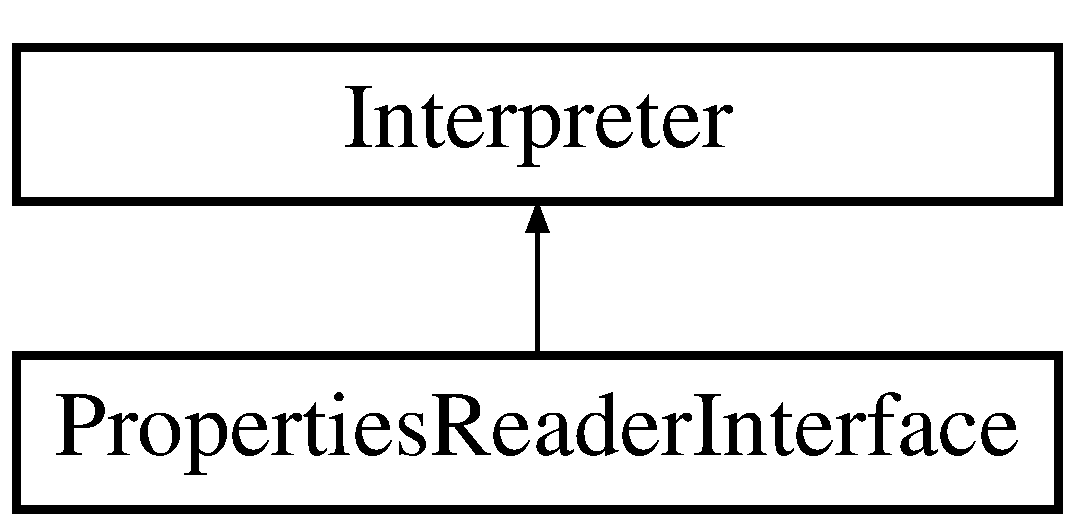
\includegraphics[height=2.000000cm]{classPropertiesReaderInterface}
\end{center}
\end{figure}
\subsection*{Public Member Functions}
\begin{DoxyCompactItemize}
\item 
\hypertarget{classPropertiesReaderInterface_a092db49483a5f97b1eb6e2fdca5b97fb}{virtual bool \hyperlink{classPropertiesReaderInterface_a092db49483a5f97b1eb6e2fdca5b97fb}{opt\-\_\-exist} (std\-::string key)=0}\label{classPropertiesReaderInterface_a092db49483a5f97b1eb6e2fdca5b97fb}

\begin{DoxyCompactList}\small\item\em Does a key exist? \end{DoxyCompactList}\item 
\hypertarget{classPropertiesReaderInterface_a16db6a1917d0274811a499b2a270679b}{virtual std\-::string \hyperlink{classPropertiesReaderInterface_a16db6a1917d0274811a499b2a270679b}{get\-\_\-opt} (std\-::string key)=0}\label{classPropertiesReaderInterface_a16db6a1917d0274811a499b2a270679b}

\begin{DoxyCompactList}\small\item\em Get an option by key. \end{DoxyCompactList}\item 
\hypertarget{classPropertiesReaderInterface_ab088ce690f3f96b3f885d762289c23c2}{virtual bool {\bfseries list\-\_\-exist} (std\-::string key)=0}\label{classPropertiesReaderInterface_ab088ce690f3f96b3f885d762289c23c2}

\item 
\hypertarget{classPropertiesReaderInterface_a466f88254dc3f26691e73ba739bdabce}{virtual std\-::vector$<$ std\-::string $>$ {\bfseries get\-\_\-list} (std\-::string key)=0}\label{classPropertiesReaderInterface_a466f88254dc3f26691e73ba739bdabce}

\end{DoxyCompactItemize}


\subsection{Detailed Description}
\hyperlink{classPropertiesReaderInterface}{Properties\-Reader\-Interface}. 

Here we create a new interpreter by passing in a single argument, the address of a properties file. This file is opened and read, with properties in the form\-: property\-\_\-name=property\-\_\-value This also accepts lists in the form -\/list\-\_\-name-\/list\-\_\-value -\/list\-\_\-name-\/list\-\_\-value2 

The documentation for this class was generated from the following file\-:\begin{DoxyCompactItemize}
\item 
lib/include/factory/properties\-\_\-reader\-\_\-interface.\-h\end{DoxyCompactItemize}

\hypertarget{classPropertyReaderFactory}{}\section{Property\+Reader\+Factory Class Reference}
\label{classPropertyReaderFactory}\index{Property\+Reader\+Factory@{Property\+Reader\+Factory}}


The Property File Reader Service Component Factory.  




{\ttfamily \#include $<$factory\+\_\+props.\+h$>$}

\subsection*{Public Member Functions}
\begin{DoxyCompactItemize}
\item 
\hyperlink{classPropertyReaderFactory_a0248347551aa31756cf3103a6677a1cb}{Property\+Reader\+Factory} ()\hypertarget{classPropertyReaderFactory_a0248347551aa31756cf3103a6677a1cb}{}\label{classPropertyReaderFactory_a0248347551aa31756cf3103a6677a1cb}

\begin{DoxyCompactList}\small\item\em Create a new Service Component Factory. \end{DoxyCompactList}\item 
\hyperlink{classPropertyReaderFactory_a9479b2681b7b0eb1332aa03715e4c34c}{$\sim$\+Property\+Reader\+Factory} ()\hypertarget{classPropertyReaderFactory_a9479b2681b7b0eb1332aa03715e4c34c}{}\label{classPropertyReaderFactory_a9479b2681b7b0eb1332aa03715e4c34c}

\begin{DoxyCompactList}\small\item\em Delete a Service Component Factory. \end{DoxyCompactList}\item 
\hyperlink{classPropertiesReaderInterface}{Properties\+Reader\+Interface} $\ast$ \hyperlink{classPropertyReaderFactory_a45379e69c4a5a247233cdb17a32f3d1e}{get\+\_\+properties\+\_\+reader\+\_\+interface} (std\+::string filename)\hypertarget{classPropertyReaderFactory_a45379e69c4a5a247233cdb17a32f3d1e}{}\label{classPropertyReaderFactory_a45379e69c4a5a247233cdb17a32f3d1e}

\begin{DoxyCompactList}\small\item\em Get a Properties File Interface Instance. \end{DoxyCompactList}\end{DoxyCompactItemize}


\subsection{Detailed Description}
The Property File Reader Service Component Factory. 

The Service Component Factory tracks the Property File Reader objects exposed by the framework and passes back instances of interfaces. This allows for the publicly exposed methods to be independent of the implementations. 

The documentation for this class was generated from the following file\+:\begin{DoxyCompactItemize}
\item 
aossl/properties/include/factory\+\_\+props.\+h\end{DoxyCompactItemize}

\hypertarget{classRedisComponentFactory}{}\section{Redis\+Component\+Factory Class Reference}
\label{classRedisComponentFactory}\index{Redis\+Component\+Factory@{Redis\+Component\+Factory}}


The Redis Service Component Factory.  




{\ttfamily \#include $<$factory\+\_\+redis.\+h$>$}

\subsection*{Public Member Functions}
\begin{DoxyCompactItemize}
\item 
\hyperlink{classRedisComponentFactory_a4c51f92cdb5da1150476178d9f5ba970}{Redis\+Component\+Factory} ()\hypertarget{classRedisComponentFactory_a4c51f92cdb5da1150476178d9f5ba970}{}\label{classRedisComponentFactory_a4c51f92cdb5da1150476178d9f5ba970}

\begin{DoxyCompactList}\small\item\em Create a new Service Component Factory. \end{DoxyCompactList}\item 
\hyperlink{classRedisComponentFactory_adacdc2aa778f3efc793743557f1fb835}{$\sim$\+Redis\+Component\+Factory} ()\hypertarget{classRedisComponentFactory_adacdc2aa778f3efc793743557f1fb835}{}\label{classRedisComponentFactory_adacdc2aa778f3efc793743557f1fb835}

\begin{DoxyCompactList}\small\item\em Delete a Service Component Factory. \end{DoxyCompactList}\item 
\hyperlink{classRedisInterface}{Redis\+Interface} $\ast$ \hyperlink{classRedisComponentFactory_a86835044e78c217f480243a3743c09e3}{get\+\_\+redis\+\_\+interface} (std\+::string hostname, int port, int timeout\+\_\+seconds, int timeout\+\_\+microseconds)\hypertarget{classRedisComponentFactory_a86835044e78c217f480243a3743c09e3}{}\label{classRedisComponentFactory_a86835044e78c217f480243a3743c09e3}

\begin{DoxyCompactList}\small\item\em Get a Redis Interface Instance. \end{DoxyCompactList}\item 
\hyperlink{classRedisInterface}{Redis\+Interface} $\ast$ \hyperlink{classRedisComponentFactory_adbb025ff948be7a72da75c863974369b}{get\+\_\+redis\+\_\+interface} (std\+::string hostname, int port)\hypertarget{classRedisComponentFactory_adbb025ff948be7a72da75c863974369b}{}\label{classRedisComponentFactory_adbb025ff948be7a72da75c863974369b}

\begin{DoxyCompactList}\small\item\em Get a Redis Interface Instance. \end{DoxyCompactList}\item 
\hyperlink{classRedisInterface}{Redis\+Interface} $\ast$ \hyperlink{classRedisComponentFactory_a92f73527a54437cf08743d2912905ead}{get\+\_\+redis\+\_\+interface} (std\+::string hostname, int port, int pool\+\_\+size)\hypertarget{classRedisComponentFactory_a92f73527a54437cf08743d2912905ead}{}\label{classRedisComponentFactory_a92f73527a54437cf08743d2912905ead}

\begin{DoxyCompactList}\small\item\em Get a Redis Interface Instance. \end{DoxyCompactList}\item 
\hyperlink{classRedisInterface}{Redis\+Interface} $\ast$ \hyperlink{classRedisComponentFactory_a5d57cf70da6c5420b419a9921ff60d8d}{get\+\_\+redis\+\_\+interface} (std\+::string hostname, int port, int timeout\+\_\+seconds, int timeout\+\_\+microseconds, int pool\+\_\+size)\hypertarget{classRedisComponentFactory_a5d57cf70da6c5420b419a9921ff60d8d}{}\label{classRedisComponentFactory_a5d57cf70da6c5420b419a9921ff60d8d}

\begin{DoxyCompactList}\small\item\em Get a Redis Interface Instance. \end{DoxyCompactList}\item 
\hyperlink{classRedisInterface}{Redis\+Interface} $\ast$ \hyperlink{classRedisComponentFactory_ad4339f7c25961aa218f41dcd4bb09003}{get\+\_\+redis\+\_\+interface} (\hyperlink{structRedisConnChain}{Redis\+Conn\+Chain} connection\+\_\+list)\hypertarget{classRedisComponentFactory_ad4339f7c25961aa218f41dcd4bb09003}{}\label{classRedisComponentFactory_ad4339f7c25961aa218f41dcd4bb09003}

\begin{DoxyCompactList}\small\item\em Get a Redis Interface Instance. \end{DoxyCompactList}\item 
\hyperlink{classRedisInterface}{Redis\+Interface} $\ast$ \hyperlink{classRedisComponentFactory_a255dea42505a6902420dae023c918554}{get\+\_\+redis\+\_\+interface} (\hyperlink{structRedisConnChain}{Redis\+Conn\+Chain} connection\+\_\+list, int pool\+\_\+size)\hypertarget{classRedisComponentFactory_a255dea42505a6902420dae023c918554}{}\label{classRedisComponentFactory_a255dea42505a6902420dae023c918554}

\begin{DoxyCompactList}\small\item\em Get a Redis Interface Instance. \end{DoxyCompactList}\end{DoxyCompactItemize}


\subsection{Detailed Description}
The Redis Service Component Factory. 

The Service Component Factory tracks the Redis objects exposed by the framework and passes back instances of interfaces. This allows for the publicly exposed methods to be independent of the implementations. 

The documentation for this class was generated from the following file\+:\begin{DoxyCompactItemize}
\item 
aossl/redis/include/factory\+\_\+redis.\+h\end{DoxyCompactItemize}

\hypertarget{structRedisConnChain}{\section{Redis\-Conn\-Chain Struct Reference}
\label{structRedisConnChain}\index{Redis\-Conn\-Chain@{Redis\-Conn\-Chain}}
}


A Structure for storing Redis Connection Information.  




{\ttfamily \#include $<$redis\-\_\-interface.\-h$>$}

\subsection*{Public Attributes}
\begin{DoxyCompactItemize}
\item 
\hypertarget{structRedisConnChain_a4694dc63aa9ea1864ddd3bd32324a517}{std\-::string {\bfseries ip}}\label{structRedisConnChain_a4694dc63aa9ea1864ddd3bd32324a517}

\item 
\hypertarget{structRedisConnChain_a5cc9c60a354a6519ab6738a97a30acf9}{int {\bfseries port}}\label{structRedisConnChain_a5cc9c60a354a6519ab6738a97a30acf9}

\item 
\hypertarget{structRedisConnChain_a8bbae840be9aab68e4c98f813915b44c}{std\-::string {\bfseries password}}\label{structRedisConnChain_a8bbae840be9aab68e4c98f813915b44c}

\item 
\hypertarget{structRedisConnChain_a9d8d3258596c3de62a7a71207df2617f}{int {\bfseries pool\-\_\-size}}\label{structRedisConnChain_a9d8d3258596c3de62a7a71207df2617f}

\item 
\hypertarget{structRedisConnChain_aa8503e6bf1350950dda24ad76cd48e24}{int {\bfseries timeout}}\label{structRedisConnChain_aa8503e6bf1350950dda24ad76cd48e24}

\item 
\hypertarget{structRedisConnChain_a92766bf2d64183f8e56515302215b4be}{int {\bfseries role}}\label{structRedisConnChain_a92766bf2d64183f8e56515302215b4be}

\end{DoxyCompactItemize}


\subsection{Detailed Description}
A Structure for storing Redis Connection Information. 

The documentation for this struct was generated from the following file\-:\begin{DoxyCompactItemize}
\item 
lib/include/factory/redis\-\_\-interface.\-h\end{DoxyCompactItemize}

\hypertarget{structRedisConnectionException}{\section{Redis\-Connection\-Exception Struct Reference}
\label{structRedisConnectionException}\index{Redis\-Connection\-Exception@{Redis\-Connection\-Exception}}
}


An Implementation of std\-::exception that denotes a connection error within Redis.  




{\ttfamily \#include $<$redis\-\_\-interface.\-h$>$}

Inheritance diagram for Redis\-Connection\-Exception\-:\begin{figure}[H]
\begin{center}
\leavevmode
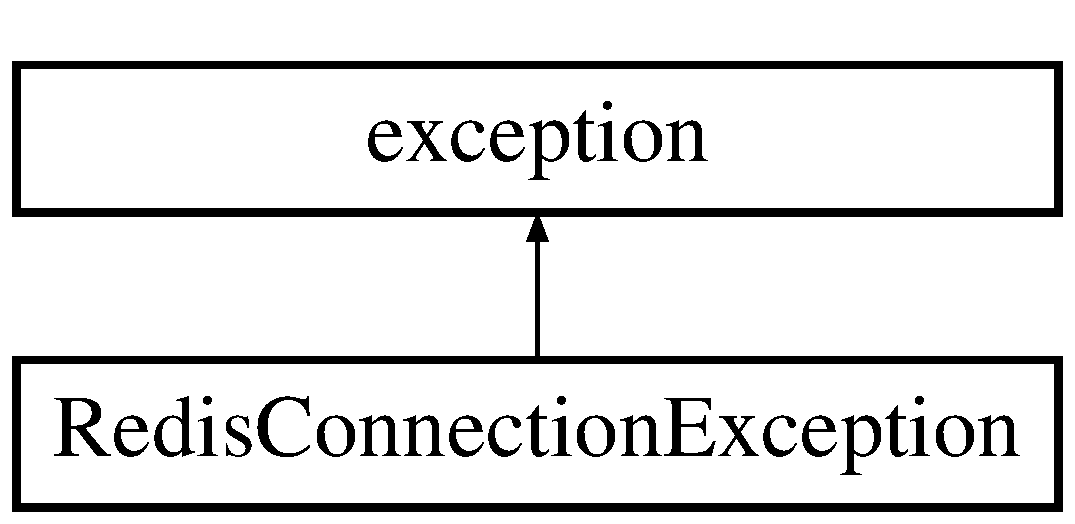
\includegraphics[height=2.000000cm]{structRedisConnectionException}
\end{center}
\end{figure}
\subsection*{Public Member Functions}
\begin{DoxyCompactItemize}
\item 
\hypertarget{structRedisConnectionException_a1a28a564f37ca6c032222fc57611fe7d}{\hyperlink{structRedisConnectionException_a1a28a564f37ca6c032222fc57611fe7d}{Redis\-Connection\-Exception} (std\-::string msg)}\label{structRedisConnectionException_a1a28a564f37ca6c032222fc57611fe7d}

\begin{DoxyCompactList}\small\item\em Create a Redis Connection Exception, and store the given error message. \end{DoxyCompactList}\item 
\hypertarget{structRedisConnectionException_a5af84b976ba7c84d4891c8b42d0c0b34}{\hyperlink{structRedisConnectionException_a5af84b976ba7c84d4891c8b42d0c0b34}{Redis\-Connection\-Exception} (const char $\ast$msg\-\_\-cstr)}\label{structRedisConnectionException_a5af84b976ba7c84d4891c8b42d0c0b34}

\begin{DoxyCompactList}\small\item\em Create a Redis Connection Exception, and store the given error message. \end{DoxyCompactList}\item 
\hypertarget{structRedisConnectionException_a309897cb6e68eea573b2db478543cb16}{const char $\ast$ \hyperlink{structRedisConnectionException_a309897cb6e68eea573b2db478543cb16}{what} () const   throw ()}\label{structRedisConnectionException_a309897cb6e68eea573b2db478543cb16}

\begin{DoxyCompactList}\small\item\em Show the error message in readable format. \end{DoxyCompactList}\end{DoxyCompactItemize}
\subsection*{Public Attributes}
\begin{DoxyCompactItemize}
\item 
\hypertarget{structRedisConnectionException_a95af5cf7df2c6dda75b37574a6cafba4}{std\-::string \hyperlink{structRedisConnectionException_a95af5cf7df2c6dda75b37574a6cafba4}{int\-\_\-msg}}\label{structRedisConnectionException_a95af5cf7df2c6dda75b37574a6cafba4}

\begin{DoxyCompactList}\small\item\em An error message passed on initialization. \end{DoxyCompactList}\end{DoxyCompactItemize}


\subsection{Detailed Description}
An Implementation of std\-::exception that denotes a connection error within Redis. 

The documentation for this struct was generated from the following file\-:\begin{DoxyCompactItemize}
\item 
lib/include/factory/redis\-\_\-interface.\-h\end{DoxyCompactItemize}

\hypertarget{classRedisInterface}{\section{Redis\-Interface Class Reference}
\label{classRedisInterface}\index{Redis\-Interface@{Redis\-Interface}}
}


The X\-Redis Admin.  




{\ttfamily \#include $<$redis\-\_\-interface.\-h$>$}

Inheritance diagram for Redis\-Interface\-:\begin{figure}[H]
\begin{center}
\leavevmode
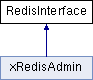
\includegraphics[height=2.000000cm]{classRedisInterface}
\end{center}
\end{figure}
\subsection*{Public Member Functions}
\begin{DoxyCompactItemize}
\item 
\hypertarget{classRedisInterface_afd325866fd98ca6e002b2702e5566ee5}{virtual std\-::string \hyperlink{classRedisInterface_afd325866fd98ca6e002b2702e5566ee5}{load} (const char $\ast$key)=0}\label{classRedisInterface_afd325866fd98ca6e002b2702e5566ee5}

\begin{DoxyCompactList}\small\item\em Load a value from Redis. \end{DoxyCompactList}\item 
\hypertarget{classRedisInterface_adb0d6e3f8a0848cbb6b346e57aeb3ad5}{virtual bool \hyperlink{classRedisInterface_adb0d6e3f8a0848cbb6b346e57aeb3ad5}{save} (const char $\ast$key, std\-::string msg)=0}\label{classRedisInterface_adb0d6e3f8a0848cbb6b346e57aeb3ad5}

\begin{DoxyCompactList}\small\item\em Save a value to Redis. \end{DoxyCompactList}\item 
\hypertarget{classRedisInterface_a3881f54b919852b7aaa231015775544e}{virtual bool \hyperlink{classRedisInterface_a3881f54b919852b7aaa231015775544e}{exists} (const char $\ast$key)=0}\label{classRedisInterface_a3881f54b919852b7aaa231015775544e}

\begin{DoxyCompactList}\small\item\em Does a key exist in Redis? \end{DoxyCompactList}\item 
\hypertarget{classRedisInterface_abb9b1fe2c11911648d62d431968fa04e}{virtual bool \hyperlink{classRedisInterface_abb9b1fe2c11911648d62d431968fa04e}{del} (const char $\ast$key)=0}\label{classRedisInterface_abb9b1fe2c11911648d62d431968fa04e}

\begin{DoxyCompactList}\small\item\em Delete a value from Redis. \end{DoxyCompactList}\item 
\hypertarget{classRedisInterface_ac327841b5c3d227be88f164495e32dd0}{virtual bool \hyperlink{classRedisInterface_ac327841b5c3d227be88f164495e32dd0}{expire} (const char $\ast$key, unsigned int second)=0}\label{classRedisInterface_ac327841b5c3d227be88f164495e32dd0}

\begin{DoxyCompactList}\small\item\em Expire a value in Redis after a specified number of seconds. \end{DoxyCompactList}\end{DoxyCompactItemize}


\subsection{Detailed Description}
The X\-Redis Admin. 

The X\-Redis Admin is responsible for all interactions with the Redis Key-\/\-Value Store. This is capable of connecting to single Redis instances or Clusters 

The documentation for this class was generated from the following file\-:\begin{DoxyCompactItemize}
\item 
lib/include/factory/redis\-\_\-interface.\-h\end{DoxyCompactItemize}

\hypertarget{structRedisKvPair}{\section{Redis\-Kv\-Pair Struct Reference}
\label{structRedisKvPair}\index{Redis\-Kv\-Pair@{Redis\-Kv\-Pair}}
}


A Structure for storing a Key-\/\-Value pair, used with batch operations.  




{\ttfamily \#include $<$redis\-\_\-interface.\-h$>$}

\subsection*{Public Attributes}
\begin{DoxyCompactItemize}
\item 
\hypertarget{structRedisKvPair_af3f52908debaab15e1ed092801d9a875}{std\-::string \hyperlink{structRedisKvPair_af3f52908debaab15e1ed092801d9a875}{key}}\label{structRedisKvPair_af3f52908debaab15e1ed092801d9a875}

\begin{DoxyCompactList}\small\item\em Key of the pair. \end{DoxyCompactList}\item 
\hypertarget{structRedisKvPair_a4d376aa2e230347adc28ac942e3da043}{std\-::string \hyperlink{structRedisKvPair_a4d376aa2e230347adc28ac942e3da043}{val}}\label{structRedisKvPair_a4d376aa2e230347adc28ac942e3da043}

\begin{DoxyCompactList}\small\item\em Value stored in the pair. \end{DoxyCompactList}\end{DoxyCompactItemize}


\subsection{Detailed Description}
A Structure for storing a Key-\/\-Value pair, used with batch operations. 

The documentation for this struct was generated from the following file\-:\begin{DoxyCompactItemize}
\item 
lib/include/factory/redis\-\_\-interface.\-h\end{DoxyCompactItemize}

\hypertarget{structRedisOperationException}{}\section{Redis\+Operation\+Exception Struct Reference}
\label{structRedisOperationException}\index{Redis\+Operation\+Exception@{Redis\+Operation\+Exception}}


An Implementation of std\+::exception that denotes an error within Redis during a transaction.  




{\ttfamily \#include $<$redis\+\_\+interface.\+h$>$}



Inheritance diagram for Redis\+Operation\+Exception\+:
\nopagebreak
\begin{figure}[H]
\begin{center}
\leavevmode
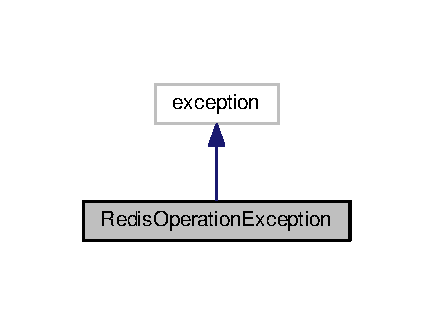
\includegraphics[width=208pt]{structRedisOperationException__inherit__graph}
\end{center}
\end{figure}


Collaboration diagram for Redis\+Operation\+Exception\+:
\nopagebreak
\begin{figure}[H]
\begin{center}
\leavevmode
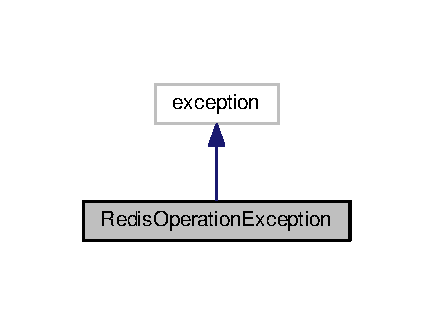
\includegraphics[width=208pt]{structRedisOperationException__coll__graph}
\end{center}
\end{figure}
\subsection*{Public Member Functions}
\begin{DoxyCompactItemize}
\item 
\hyperlink{structRedisOperationException_a54e07b6a7c4d81ab0cb4d1f61d5a6226}{Redis\+Operation\+Exception} (std\+::string msg)\hypertarget{structRedisOperationException_a54e07b6a7c4d81ab0cb4d1f61d5a6226}{}\label{structRedisOperationException_a54e07b6a7c4d81ab0cb4d1f61d5a6226}

\begin{DoxyCompactList}\small\item\em Create a Redis Operation Exception, and store the given error message. \end{DoxyCompactList}\item 
\hyperlink{structRedisOperationException_a330513962eb439159cf494f3996edc8c}{Redis\+Operation\+Exception} (const char $\ast$msg\+\_\+cstr)\hypertarget{structRedisOperationException_a330513962eb439159cf494f3996edc8c}{}\label{structRedisOperationException_a330513962eb439159cf494f3996edc8c}

\begin{DoxyCompactList}\small\item\em Create a Redis Operation Exception, and store the given error message. \end{DoxyCompactList}\item 
const char $\ast$ \hyperlink{structRedisOperationException_a629e013517496f9e14ae5286a8759043}{what} () const   throw ()\hypertarget{structRedisOperationException_a629e013517496f9e14ae5286a8759043}{}\label{structRedisOperationException_a629e013517496f9e14ae5286a8759043}

\begin{DoxyCompactList}\small\item\em Show the error message in readable format. \end{DoxyCompactList}\end{DoxyCompactItemize}
\subsection*{Public Attributes}
\begin{DoxyCompactItemize}
\item 
std\+::string \hyperlink{structRedisOperationException_ac5deeab2028bb95e7db928cfb222656e}{int\+\_\+msg}\hypertarget{structRedisOperationException_ac5deeab2028bb95e7db928cfb222656e}{}\label{structRedisOperationException_ac5deeab2028bb95e7db928cfb222656e}

\begin{DoxyCompactList}\small\item\em An error message passed on initialization. \end{DoxyCompactList}\end{DoxyCompactItemize}


\subsection{Detailed Description}
An Implementation of std\+::exception that denotes an error within Redis during a transaction. 

The documentation for this struct was generated from the following file\+:\begin{DoxyCompactItemize}
\item 
aossl/redis/include/redis\+\_\+interface.\+h\end{DoxyCompactItemize}

\hypertarget{classResultsIteratorInterface}{\section{Results\-Iterator\-Interface Class Reference}
\label{classResultsIteratorInterface}\index{Results\-Iterator\-Interface@{Results\-Iterator\-Interface}}
}


Results Iterator for viewing query results.  




{\ttfamily \#include $<$neo4j\-\_\-interface.\-h$>$}

\subsection*{Public Member Functions}
\begin{DoxyCompactItemize}
\item 
\hypertarget{classResultsIteratorInterface_a4f6574b8a57dbd2ea3c86e66bf260252}{virtual void \hyperlink{classResultsIteratorInterface_a4f6574b8a57dbd2ea3c86e66bf260252}{clear} ()=0}\label{classResultsIteratorInterface_a4f6574b8a57dbd2ea3c86e66bf260252}

\begin{DoxyCompactList}\small\item\em Clear the results iterator of all values. \end{DoxyCompactList}\item 
virtual bool \hyperlink{classResultsIteratorInterface_ab00e99e5bd9f186eb9bdcdf30d594b99}{empty} ()=0
\begin{DoxyCompactList}\small\item\em Is the iterator empty? \end{DoxyCompactList}\item 
\hypertarget{classResultsIteratorInterface_a9a022aba2a3e7771c8d147885ca151dd}{virtual unsigned int \hyperlink{classResultsIteratorInterface_a9a022aba2a3e7771c8d147885ca151dd}{length} ()=0}\label{classResultsIteratorInterface_a9a022aba2a3e7771c8d147885ca151dd}

\begin{DoxyCompactList}\small\item\em Get the number of results in the query. \end{DoxyCompactList}\item 
\hypertarget{classResultsIteratorInterface_a00385bfa8ddabb267cf46006a9a0f6e9}{virtual \hyperlink{classResultTreeInterface}{Result\-Tree\-Interface} $\ast$ \hyperlink{classResultsIteratorInterface_a00385bfa8ddabb267cf46006a9a0f6e9}{next} ()=0}\label{classResultsIteratorInterface_a00385bfa8ddabb267cf46006a9a0f6e9}

\begin{DoxyCompactList}\small\item\em Get the next query result. \end{DoxyCompactList}\end{DoxyCompactItemize}


\subsection{Detailed Description}
Results Iterator for viewing query results. 

Accepts a result stream as an input, returns Results Trees for each entry that matches in the query Deletes it when finished 

\subsection{Member Function Documentation}
\hypertarget{classResultsIteratorInterface_ab00e99e5bd9f186eb9bdcdf30d594b99}{\index{Results\-Iterator\-Interface@{Results\-Iterator\-Interface}!empty@{empty}}
\index{empty@{empty}!ResultsIteratorInterface@{Results\-Iterator\-Interface}}
\subsubsection[{empty}]{\setlength{\rightskip}{0pt plus 5cm}virtual bool Results\-Iterator\-Interface\-::empty (
\begin{DoxyParamCaption}
{}
\end{DoxyParamCaption}
)\hspace{0.3cm}{\ttfamily [pure virtual]}}}\label{classResultsIteratorInterface_ab00e99e5bd9f186eb9bdcdf30d594b99}


Is the iterator empty? 

Return true if this iterator contains no results. Return false otherwise. 

The documentation for this class was generated from the following file\-:\begin{DoxyCompactItemize}
\item 
lib/include/factory/neo4j\-\_\-interface.\-h\end{DoxyCompactItemize}

\hypertarget{classResultTreeInterface}{\section{Result\-Tree\-Interface Class Reference}
\label{classResultTreeInterface}\index{Result\-Tree\-Interface@{Result\-Tree\-Interface}}
}


Tree of Query Results.  




{\ttfamily \#include $<$neo4j\-\_\-interface.\-h$>$}

\subsection*{Public Member Functions}
\begin{DoxyCompactItemize}
\item 
\hypertarget{classResultTreeInterface_acc4e0493661f5f2b0b836c7a1bdb3a8f}{virtual \hyperlink{classDbObjectInterface}{Db\-Object\-Interface} $\ast$ \hyperlink{classResultTreeInterface_acc4e0493661f5f2b0b836c7a1bdb3a8f}{get} (int index)=0}\label{classResultTreeInterface_acc4e0493661f5f2b0b836c7a1bdb3a8f}

\begin{DoxyCompactList}\small\item\em Get the node/edge at the specified index. \end{DoxyCompactList}\end{DoxyCompactItemize}


\subsection{Detailed Description}
Tree of Query Results. 

The documentation for this class was generated from the following file\-:\begin{DoxyCompactItemize}
\item 
lib/include/factory/neo4j\-\_\-interface.\-h\end{DoxyCompactItemize}

\hypertarget{classServiceInterface}{}\section{Service\+Interface Class Reference}
\label{classServiceInterface}\index{Service\+Interface@{Service\+Interface}}


A Service class which can be registered with Consul for each instance of a particular service.  




{\ttfamily \#include $<$consul\+\_\+interface.\+h$>$}

\subsection*{Public Member Functions}
\begin{DoxyCompactItemize}
\item 
virtual std\+::string \hyperlink{classServiceInterface_a2c041d65d3e725f1cf8e2379f4620d58}{to\+\_\+json} ()=0
\begin{DoxyCompactList}\small\item\em Convert the Service into a J\+S\+ON Message. \end{DoxyCompactList}\item 
virtual std\+::string \hyperlink{classServiceInterface_a0ba731e4d379cbeddc852304b470c617}{get\+\_\+id} ()=0\hypertarget{classServiceInterface_a0ba731e4d379cbeddc852304b470c617}{}\label{classServiceInterface_a0ba731e4d379cbeddc852304b470c617}

\begin{DoxyCompactList}\small\item\em Get the Service ID. \end{DoxyCompactList}\item 
virtual std\+::string \hyperlink{classServiceInterface_aed2140959e23f98cd0cca1a101646384}{get\+\_\+name} ()=0\hypertarget{classServiceInterface_aed2140959e23f98cd0cca1a101646384}{}\label{classServiceInterface_aed2140959e23f98cd0cca1a101646384}

\begin{DoxyCompactList}\small\item\em Get the Service Name. \end{DoxyCompactList}\item 
virtual std\+::string \hyperlink{classServiceInterface_a6c4fd6eff9e1c8eed5dfed301d2f8047}{get\+\_\+address} ()=0\hypertarget{classServiceInterface_a6c4fd6eff9e1c8eed5dfed301d2f8047}{}\label{classServiceInterface_a6c4fd6eff9e1c8eed5dfed301d2f8047}

\begin{DoxyCompactList}\small\item\em Get the Service Address. \end{DoxyCompactList}\item 
virtual std\+::string \hyperlink{classServiceInterface_a7c8a328711f7fb019a9f7dadcb897cb0}{get\+\_\+port} ()=0\hypertarget{classServiceInterface_a7c8a328711f7fb019a9f7dadcb897cb0}{}\label{classServiceInterface_a7c8a328711f7fb019a9f7dadcb897cb0}

\begin{DoxyCompactList}\small\item\em Get the Service Port. \end{DoxyCompactList}\item 
virtual void \hyperlink{classServiceInterface_aade793bb679fa00cd34194a3623c554a}{set\+\_\+id} (std\+::string new\+\_\+id)=0\hypertarget{classServiceInterface_aade793bb679fa00cd34194a3623c554a}{}\label{classServiceInterface_aade793bb679fa00cd34194a3623c554a}

\begin{DoxyCompactList}\small\item\em Set the Service ID. \end{DoxyCompactList}\item 
virtual void \hyperlink{classServiceInterface_ac9b2d1a785b665ef3c575f5877148511}{set\+\_\+name} (std\+::string new\+\_\+name)=0\hypertarget{classServiceInterface_ac9b2d1a785b665ef3c575f5877148511}{}\label{classServiceInterface_ac9b2d1a785b665ef3c575f5877148511}

\begin{DoxyCompactList}\small\item\em Set the Service Name. \end{DoxyCompactList}\item 
virtual void \hyperlink{classServiceInterface_a619fb75631f816d547d2ad3efeae2bf5}{set\+\_\+address} (std\+::string new\+\_\+address)=0\hypertarget{classServiceInterface_a619fb75631f816d547d2ad3efeae2bf5}{}\label{classServiceInterface_a619fb75631f816d547d2ad3efeae2bf5}

\begin{DoxyCompactList}\small\item\em Set the Service Address. \end{DoxyCompactList}\item 
virtual void \hyperlink{classServiceInterface_a2c9385fbc567949560dc7972e6a7059e}{set\+\_\+port} (std\+::string new\+\_\+port)=0\hypertarget{classServiceInterface_a2c9385fbc567949560dc7972e6a7059e}{}\label{classServiceInterface_a2c9385fbc567949560dc7972e6a7059e}

\begin{DoxyCompactList}\small\item\em Set the Service Port. \end{DoxyCompactList}\item 
virtual std\+::vector$<$ std\+::string $>$ \hyperlink{classServiceInterface_afdc1ce12ef5ff09cf82e3d0f8ea7724a}{get\+\_\+tags} ()=0\hypertarget{classServiceInterface_afdc1ce12ef5ff09cf82e3d0f8ea7724a}{}\label{classServiceInterface_afdc1ce12ef5ff09cf82e3d0f8ea7724a}

\begin{DoxyCompactList}\small\item\em Get the tags. \end{DoxyCompactList}\item 
virtual void \hyperlink{classServiceInterface_ac8b80c9301fa04ea295acecd88b9cc42}{add\+\_\+tag} (std\+::string new\+\_\+tag)=0\hypertarget{classServiceInterface_ac8b80c9301fa04ea295acecd88b9cc42}{}\label{classServiceInterface_ac8b80c9301fa04ea295acecd88b9cc42}

\begin{DoxyCompactList}\small\item\em Add a tag. \end{DoxyCompactList}\item 
virtual void \hyperlink{classServiceInterface_a3e27c216421be0e92984b07a095f1279}{clear\+\_\+tags} ()=0\hypertarget{classServiceInterface_a3e27c216421be0e92984b07a095f1279}{}\label{classServiceInterface_a3e27c216421be0e92984b07a095f1279}

\begin{DoxyCompactList}\small\item\em Clear the tags. \end{DoxyCompactList}\item 
virtual int \hyperlink{classServiceInterface_aad0434e39242a47048659a1243fab46e}{num\+\_\+tags} () const =0\hypertarget{classServiceInterface_aad0434e39242a47048659a1243fab46e}{}\label{classServiceInterface_aad0434e39242a47048659a1243fab46e}

\begin{DoxyCompactList}\small\item\em How many tags are there? \end{DoxyCompactList}\item 
virtual \hyperlink{structHealthCheck}{Health\+Check} \hyperlink{classServiceInterface_afa5e0a43120dcd89dfcf7ae8aa086217}{get\+\_\+check} ()=0\hypertarget{classServiceInterface_afa5e0a43120dcd89dfcf7ae8aa086217}{}\label{classServiceInterface_afa5e0a43120dcd89dfcf7ae8aa086217}

\begin{DoxyCompactList}\small\item\em Get the health checks. \end{DoxyCompactList}\item 
virtual void \hyperlink{classServiceInterface_a32065df2094fa5a53708f5ff3944195b}{set\+\_\+check} (std\+::string scr, int interval\+\_\+seconds)=0\hypertarget{classServiceInterface_a32065df2094fa5a53708f5ff3944195b}{}\label{classServiceInterface_a32065df2094fa5a53708f5ff3944195b}

\begin{DoxyCompactList}\small\item\em Add a check. \end{DoxyCompactList}\end{DoxyCompactItemize}


\subsection{Detailed Description}
A Service class which can be registered with Consul for each instance of a particular service. 

An instance of this class can be instantiated by a service and is passed to the consul admin to register and de-\/register 

\subsection{Member Function Documentation}
\index{Service\+Interface@{Service\+Interface}!to\+\_\+json@{to\+\_\+json}}
\index{to\+\_\+json@{to\+\_\+json}!Service\+Interface@{Service\+Interface}}
\subsubsection[{\texorpdfstring{to\+\_\+json()=0}{to_json()=0}}]{\setlength{\rightskip}{0pt plus 5cm}virtual std\+::string Service\+Interface\+::to\+\_\+json (
\begin{DoxyParamCaption}
{}
\end{DoxyParamCaption}
)\hspace{0.3cm}{\ttfamily [pure virtual]}}\hypertarget{classServiceInterface_a2c041d65d3e725f1cf8e2379f4620d58}{}\label{classServiceInterface_a2c041d65d3e725f1cf8e2379f4620d58}


Convert the Service into a J\+S\+ON Message. 

Method that allows the service to be transformed into a json message that can be sent via H\+T\+TP to a Consul instance 

The documentation for this class was generated from the following file\+:\begin{DoxyCompactItemize}
\item 
aossl/consul/include/consul\+\_\+interface.\+h\end{DoxyCompactItemize}

\hypertarget{classuuidComponentFactory}{}\section{uuid\+Component\+Factory Class Reference}
\label{classuuidComponentFactory}\index{uuid\+Component\+Factory@{uuid\+Component\+Factory}}


The U\+U\+ID Service Component Factory.  




{\ttfamily \#include $<$factory\+\_\+uuid.\+h$>$}

\subsection*{Public Member Functions}
\begin{DoxyCompactItemize}
\item 
\hyperlink{classuuidComponentFactory_a6dc50b685a22da9b64b137de800365f4}{uuid\+Component\+Factory} ()\hypertarget{classuuidComponentFactory_a6dc50b685a22da9b64b137de800365f4}{}\label{classuuidComponentFactory_a6dc50b685a22da9b64b137de800365f4}

\begin{DoxyCompactList}\small\item\em Create a new Service Component Factory. \end{DoxyCompactList}\item 
\hyperlink{classuuidComponentFactory_a64f6dccee4aa0f93ee322d2541bb8103}{$\sim$uuid\+Component\+Factory} ()\hypertarget{classuuidComponentFactory_a64f6dccee4aa0f93ee322d2541bb8103}{}\label{classuuidComponentFactory_a64f6dccee4aa0f93ee322d2541bb8103}

\begin{DoxyCompactList}\small\item\em Delete a Service Component Factory. \end{DoxyCompactList}\item 
\hyperlink{classuuidInterface}{uuid\+Interface} $\ast$ \hyperlink{classuuidComponentFactory_a50e1f856aa001a732a324370983ca236}{get\+\_\+uuid\+\_\+interface} ()\hypertarget{classuuidComponentFactory_a50e1f856aa001a732a324370983ca236}{}\label{classuuidComponentFactory_a50e1f856aa001a732a324370983ca236}

\begin{DoxyCompactList}\small\item\em Get the U\+U\+ID Interface instance. \end{DoxyCompactList}\end{DoxyCompactItemize}


\subsection{Detailed Description}
The U\+U\+ID Service Component Factory. 

The Service Component Factory tracks the U\+U\+ID objects exposed by the framework and passes back instances of interfaces. This allows for the publicly exposed methods to be independent of the implementations. 

The documentation for this class was generated from the following file\+:\begin{DoxyCompactItemize}
\item 
aossl/uuid/include/factory\+\_\+uuid.\+h\end{DoxyCompactItemize}

\hypertarget{structUuidContainer}{}\section{Uuid\+Container Struct Reference}
\label{structUuidContainer}\index{Uuid\+Container@{Uuid\+Container}}


A return structure which captures any security error messages thrown by the framework.  




{\ttfamily \#include $<$uuid\+\_\+interface.\+h$>$}

\subsection*{Public Attributes}
\begin{DoxyCompactItemize}
\item 
std\+::string \hyperlink{structUuidContainer_aea2f6e3768858acb4086cd1a93c5666a}{id}\hypertarget{structUuidContainer_aea2f6e3768858acb4086cd1a93c5666a}{}\label{structUuidContainer_aea2f6e3768858acb4086cd1a93c5666a}

\begin{DoxyCompactList}\small\item\em The U\+U\+ID generated. \end{DoxyCompactList}\item 
std\+::string \hyperlink{structUuidContainer_a58e21d1df4638157e157a41fa95a5e07}{err}\hypertarget{structUuidContainer_a58e21d1df4638157e157a41fa95a5e07}{}\label{structUuidContainer_a58e21d1df4638157e157a41fa95a5e07}

\begin{DoxyCompactList}\small\item\em Is either empty or contains an error message. \end{DoxyCompactList}\end{DoxyCompactItemize}


\subsection{Detailed Description}
A return structure which captures any security error messages thrown by the framework. 

The documentation for this struct was generated from the following file\+:\begin{DoxyCompactItemize}
\item 
aossl/uuid/include/uuid\+\_\+interface.\+h\end{DoxyCompactItemize}

\hypertarget{classuuidInterface}{\section{uuid\-Interface Class Reference}
\label{classuuidInterface}\index{uuid\-Interface@{uuid\-Interface}}
}


U\-U\-I\-D Admin.  




{\ttfamily \#include $<$uuid\-\_\-interface.\-h$>$}

Inheritance diagram for uuid\-Interface\-:\begin{figure}[H]
\begin{center}
\leavevmode
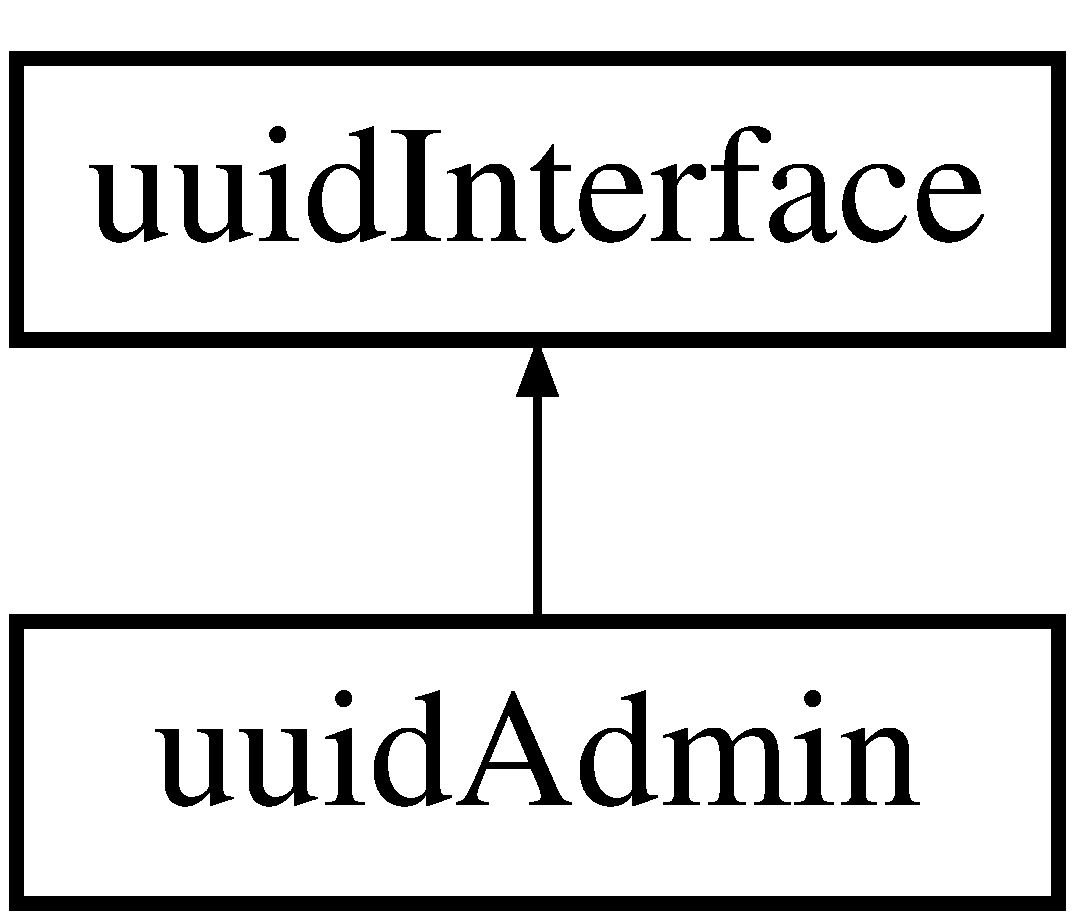
\includegraphics[height=2.000000cm]{classuuidInterface}
\end{center}
\end{figure}
\subsection*{Public Member Functions}
\begin{DoxyCompactItemize}
\item 
virtual std\-::string \hyperlink{classuuidInterface_ae1696692de5b139246154c8d32d44797}{generate} ()=0
\begin{DoxyCompactList}\small\item\em Generate a new U\-U\-I\-D. \end{DoxyCompactList}\end{DoxyCompactItemize}


\subsection{Detailed Description}
U\-U\-I\-D Admin. 

The U\-U\-I\-D Admin is in charge of generating any Universally Unique I\-D's that are required throughout program execution 

\subsection{Member Function Documentation}
\hypertarget{classuuidInterface_ae1696692de5b139246154c8d32d44797}{\index{uuid\-Interface@{uuid\-Interface}!generate@{generate}}
\index{generate@{generate}!uuidInterface@{uuid\-Interface}}
\subsubsection[{generate}]{\setlength{\rightskip}{0pt plus 5cm}virtual std\-::string uuid\-Interface\-::generate (
\begin{DoxyParamCaption}
{}
\end{DoxyParamCaption}
)\hspace{0.3cm}{\ttfamily [pure virtual]}}}\label{classuuidInterface_ae1696692de5b139246154c8d32d44797}


Generate a new U\-U\-I\-D. 

The method will generate on the means of generation present on your system In some cases, this may result in U\-U\-I\-D's being generated that pose a security risk. In this case, that fact will be clearly called out in the logs, and it is recommended that production systems are tested to ensure that U\-U\-I\-D's are generated in a safe manner 

Implemented in \hyperlink{classuuidAdmin_a344f39f4c1e15cf72e64b3544312d7ed}{uuid\-Admin}.



The documentation for this class was generated from the following file\-:\begin{DoxyCompactItemize}
\item 
lib/include/factory/uuid\-\_\-interface.\-h\end{DoxyCompactItemize}

\hypertarget{classZmqComponentFactory}{}\section{Zmq\+Component\+Factory Class Reference}
\label{classZmqComponentFactory}\index{Zmq\+Component\+Factory@{Zmq\+Component\+Factory}}


The Z\+MQ Service Component Factory.  




{\ttfamily \#include $<$factory\+\_\+zmq.\+h$>$}

\subsection*{Public Member Functions}
\begin{DoxyCompactItemize}
\item 
\hyperlink{classZmqComponentFactory_a453e53f66ed31f7d42156c4c351a8969}{Zmq\+Component\+Factory} ()\hypertarget{classZmqComponentFactory_a453e53f66ed31f7d42156c4c351a8969}{}\label{classZmqComponentFactory_a453e53f66ed31f7d42156c4c351a8969}

\begin{DoxyCompactList}\small\item\em Create a new Service Component Factory. \end{DoxyCompactList}\item 
{\bfseries Zmq\+Component\+Factory} (int num\+\_\+sockets)\hypertarget{classZmqComponentFactory_ab90c074a00528e7b475a4c212137168e}{}\label{classZmqComponentFactory_ab90c074a00528e7b475a4c212137168e}

\item 
\hyperlink{classZmqComponentFactory_a8cf8d605f3cf8a81f008549a85089adf}{$\sim$\+Zmq\+Component\+Factory} ()\hypertarget{classZmqComponentFactory_a8cf8d605f3cf8a81f008549a85089adf}{}\label{classZmqComponentFactory_a8cf8d605f3cf8a81f008549a85089adf}

\begin{DoxyCompactList}\small\item\em Delete a Service Component Factory. \end{DoxyCompactList}\item 
\hyperlink{classZmqio}{Zmqio} $\ast$ \hyperlink{classZmqComponentFactory_a17f303d9fba693b9ee69f6dc09588038}{get\+\_\+zmq\+\_\+outbound\+\_\+interface} (std\+::string conn\+\_\+str, int connection\+\_\+type)\hypertarget{classZmqComponentFactory_a17f303d9fba693b9ee69f6dc09588038}{}\label{classZmqComponentFactory_a17f303d9fba693b9ee69f6dc09588038}

\begin{DoxyCompactList}\small\item\em Get a Z\+MQ Outbound Interface instance. \end{DoxyCompactList}\item 
\hyperlink{classZmqio}{Zmqio} $\ast$ \hyperlink{classZmqComponentFactory_a37c5e3dd16c61ac581dcf6ed94525f22}{get\+\_\+zmq\+\_\+inbound\+\_\+interface} (std\+::string conn\+\_\+str, int connection\+\_\+type)\hypertarget{classZmqComponentFactory_a37c5e3dd16c61ac581dcf6ed94525f22}{}\label{classZmqComponentFactory_a37c5e3dd16c61ac581dcf6ed94525f22}

\begin{DoxyCompactList}\small\item\em Get a Z\+MQ Inbound Interface instance. \end{DoxyCompactList}\end{DoxyCompactItemize}


\subsection{Detailed Description}
The Z\+MQ Service Component Factory. 

The Service Component Factory tracks the Z\+MQ objects exposed by the framework and passes back instances of interfaces. This allows for the publicly exposed methods to be independent of the implementations. 

The documentation for this class was generated from the following file\+:\begin{DoxyCompactItemize}
\item 
aossl/zmq/include/factory\+\_\+zmq.\+h\end{DoxyCompactItemize}

\hypertarget{classZmqIn}{\section{Zmq\-In Class Reference}
\label{classZmqIn}\index{Zmq\-In@{Zmq\-In}}
}


An Inbound Z\-M\-Q Manager.  




{\ttfamily \#include $<$zmq\-\_\-interface.\-h$>$}

Inheritance diagram for Zmq\-In\-:\begin{figure}[H]
\begin{center}
\leavevmode
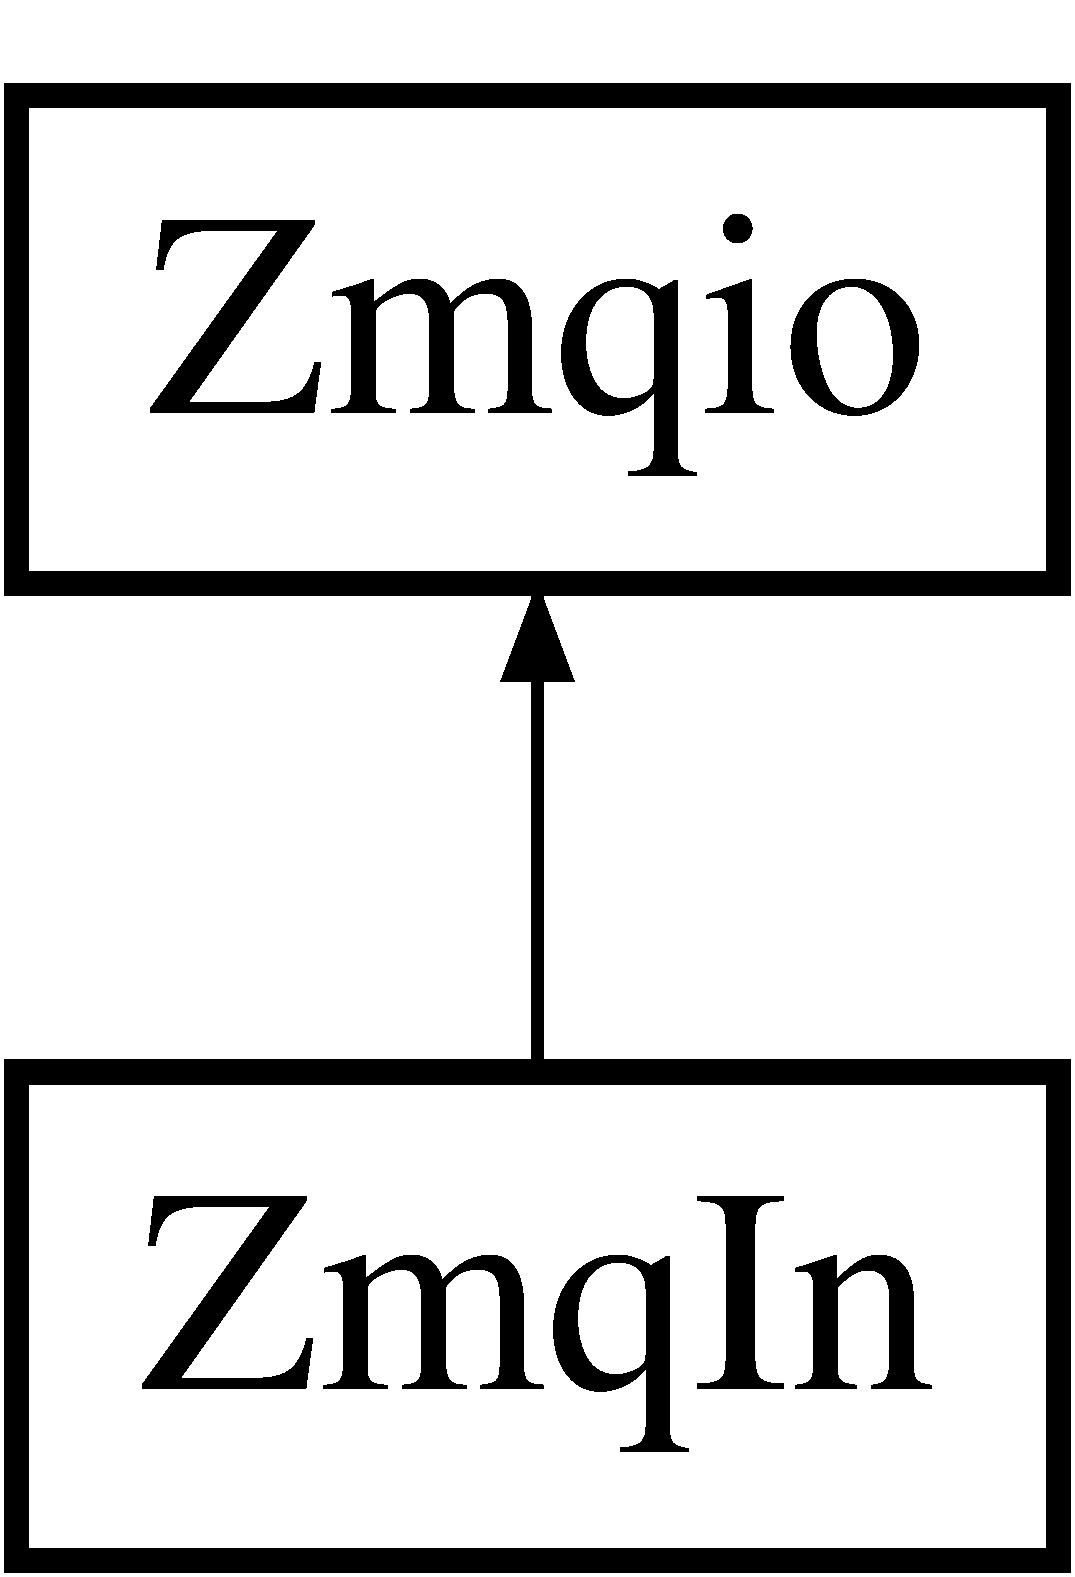
\includegraphics[height=2.000000cm]{classZmqIn}
\end{center}
\end{figure}
\subsection*{Public Member Functions}
\begin{DoxyCompactItemize}
\item 
\hypertarget{classZmqIn_ad6037a187635f7d46bab5da961156751}{virtual void \hyperlink{classZmqIn_ad6037a187635f7d46bab5da961156751}{bind} (std\-::string conn\-\_\-str)=0}\label{classZmqIn_ad6037a187635f7d46bab5da961156751}

\begin{DoxyCompactList}\small\item\em Bind on the given conn\-\_\-str. \end{DoxyCompactList}\item 
\hypertarget{classZmqIn_a375de593defd4c2cf3adebad063950fe}{virtual std\-::string \hyperlink{classZmqIn_a375de593defd4c2cf3adebad063950fe}{recv} ()=0}\label{classZmqIn_a375de593defd4c2cf3adebad063950fe}

\begin{DoxyCompactList}\small\item\em Recieve a message on the port. \end{DoxyCompactList}\item 
\hypertarget{classZmqIn_ad2a35cc76a5b0b2412fda5418f708e60}{virtual void \hyperlink{classZmqIn_ad2a35cc76a5b0b2412fda5418f708e60}{send} (const char $\ast$msg, int msg\-\_\-size)=0}\label{classZmqIn_ad2a35cc76a5b0b2412fda5418f708e60}

\begin{DoxyCompactList}\small\item\em Send a message on the port. \end{DoxyCompactList}\item 
\hypertarget{classZmqIn_adf4165c263ddc5b68099b93b9f37f592}{virtual void \hyperlink{classZmqIn_adf4165c263ddc5b68099b93b9f37f592}{send} (std\-::string msg)=0}\label{classZmqIn_adf4165c263ddc5b68099b93b9f37f592}

\begin{DoxyCompactList}\small\item\em Send a string on the port. \end{DoxyCompactList}\item 
\hypertarget{classZmqIn_a1b7ed3f43e1796a5a0cdd090f69ae932}{virtual void \hyperlink{classZmqIn_a1b7ed3f43e1796a5a0cdd090f69ae932}{subscribe} (std\-::string filter)=0}\label{classZmqIn_a1b7ed3f43e1796a5a0cdd090f69ae932}

\begin{DoxyCompactList}\small\item\em Subscribe on a particular filter (only effective for Pub/\-Sub) \end{DoxyCompactList}\end{DoxyCompactItemize}


\subsection{Detailed Description}
An Inbound Z\-M\-Q Manager. 

Acts as the Responder (Server) in the Z\-M\-Q Sockets Recieve, then Send 

The documentation for this class was generated from the following file\-:\begin{DoxyCompactItemize}
\item 
lib/include/factory/zmq\-\_\-interface.\-h\end{DoxyCompactItemize}

\hypertarget{classZmqio}{\section{Zmqio Class Reference}
\label{classZmqio}\index{Zmqio@{Zmqio}}
}


An Interface for Z\-M\-Q\-I\-O.  




{\ttfamily \#include $<$zmq\-\_\-interface.\-h$>$}

Inheritance diagram for Zmqio\-:\begin{figure}[H]
\begin{center}
\leavevmode
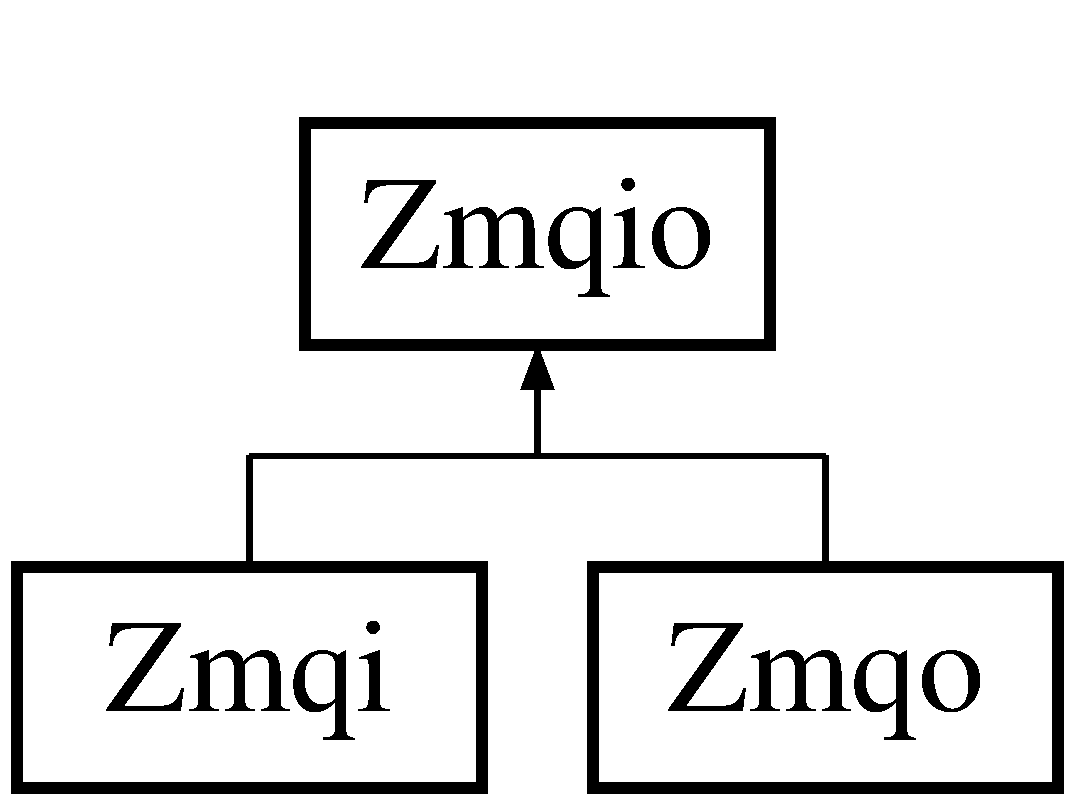
\includegraphics[height=2.000000cm]{classZmqio}
\end{center}
\end{figure}
\subsection*{Public Member Functions}
\begin{DoxyCompactItemize}
\item 
\hypertarget{classZmqio_a9365ac0ed42905898502e16857997acc}{virtual std\-::string \hyperlink{classZmqio_a9365ac0ed42905898502e16857997acc}{recv} ()=0}\label{classZmqio_a9365ac0ed42905898502e16857997acc}

\begin{DoxyCompactList}\small\item\em Recieve a message on the port. \end{DoxyCompactList}\item 
\hypertarget{classZmqio_a858e00e8ac5c4d1d60c665fa7c0716f0}{virtual void \hyperlink{classZmqio_a858e00e8ac5c4d1d60c665fa7c0716f0}{send} (const char $\ast$msg, int msg\-\_\-size)=0}\label{classZmqio_a858e00e8ac5c4d1d60c665fa7c0716f0}

\begin{DoxyCompactList}\small\item\em Send a message on the port. \end{DoxyCompactList}\item 
\hypertarget{classZmqio_a079f5752b553ddb2e5a2da565bcf162c}{virtual void \hyperlink{classZmqio_a079f5752b553ddb2e5a2da565bcf162c}{send} (std\-::string msg)=0}\label{classZmqio_a079f5752b553ddb2e5a2da565bcf162c}

\begin{DoxyCompactList}\small\item\em Send a string on the port. \end{DoxyCompactList}\item 
\hypertarget{classZmqio_aa315934401c5a3ba2eb502c16a3a6aca}{virtual void \hyperlink{classZmqio_aa315934401c5a3ba2eb502c16a3a6aca}{subscribe} (std\-::string filter)=0}\label{classZmqio_aa315934401c5a3ba2eb502c16a3a6aca}

\begin{DoxyCompactList}\small\item\em Subscribe on a particular filter (only effective for Pub/\-Sub) \end{DoxyCompactList}\end{DoxyCompactItemize}


\subsection{Detailed Description}
An Interface for Z\-M\-Q\-I\-O. 

Defines the methods that the Z\-M\-Q Managers must implement send \& recv, as well as subscribe 

The documentation for this class was generated from the following file\-:\begin{DoxyCompactItemize}
\item 
lib/include/factory/zmq\-\_\-interface.\-h\end{DoxyCompactItemize}

\hypertarget{classZmqOut}{\section{Zmq\-Out Class Reference}
\label{classZmqOut}\index{Zmq\-Out@{Zmq\-Out}}
}


An Outbound Z\-M\-Q Manager.  




{\ttfamily \#include $<$zmq\-\_\-interface.\-h$>$}

Inheritance diagram for Zmq\-Out\-:\begin{figure}[H]
\begin{center}
\leavevmode
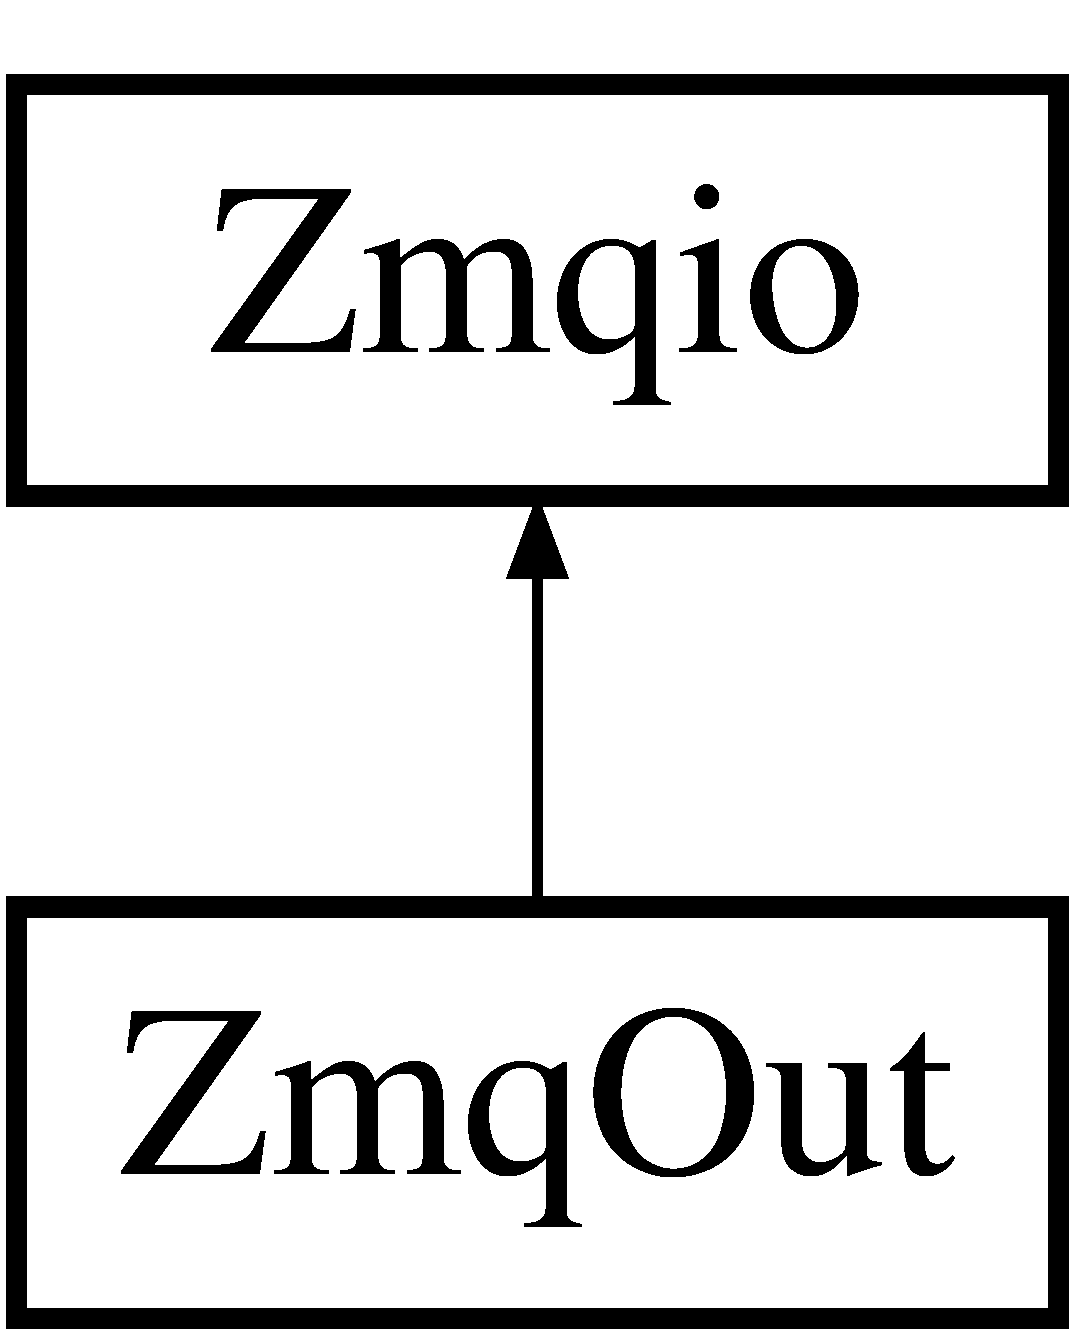
\includegraphics[height=2.000000cm]{classZmqOut}
\end{center}
\end{figure}
\subsection*{Public Member Functions}
\begin{DoxyCompactItemize}
\item 
\hypertarget{classZmqOut_ae34b1742c72e0c82ea42315cb68f1a20}{virtual void \hyperlink{classZmqOut_ae34b1742c72e0c82ea42315cb68f1a20}{connect} (std\-::string conn\-\_\-str)=0}\label{classZmqOut_ae34b1742c72e0c82ea42315cb68f1a20}

\begin{DoxyCompactList}\small\item\em Connect to the given conn\-\_\-str. \end{DoxyCompactList}\item 
\hypertarget{classZmqOut_a97935d9e7cbacd2fcb9655433e4b7af4}{virtual void \hyperlink{classZmqOut_a97935d9e7cbacd2fcb9655433e4b7af4}{send} (const char $\ast$msg, int msg\-\_\-size)=0}\label{classZmqOut_a97935d9e7cbacd2fcb9655433e4b7af4}

\begin{DoxyCompactList}\small\item\em Send a message on the port. \end{DoxyCompactList}\item 
\hypertarget{classZmqOut_ac7b314ddf6e0357c31b05fb2b1b91635}{virtual void \hyperlink{classZmqOut_ac7b314ddf6e0357c31b05fb2b1b91635}{send} (std\-::string msg)=0}\label{classZmqOut_ac7b314ddf6e0357c31b05fb2b1b91635}

\begin{DoxyCompactList}\small\item\em Send a string on the port. \end{DoxyCompactList}\item 
\hypertarget{classZmqOut_a02da5e5dd51f99e7d35a3f843b9bd00e}{virtual std\-::string \hyperlink{classZmqOut_a02da5e5dd51f99e7d35a3f843b9bd00e}{recv} ()=0}\label{classZmqOut_a02da5e5dd51f99e7d35a3f843b9bd00e}

\begin{DoxyCompactList}\small\item\em Recieve a message on the port. \end{DoxyCompactList}\end{DoxyCompactItemize}


\subsection{Detailed Description}
An Outbound Z\-M\-Q Manager. 

Acts as the Requestor (Client) in the Z\-M\-Q Sockets Send, then Recieve 

The documentation for this class was generated from the following file\-:\begin{DoxyCompactItemize}
\item 
lib/include/factory/zmq\-\_\-interface.\-h\end{DoxyCompactItemize}

%--- End generated contents ---

% Index
\backmatter
\newpage
\phantomsection
\clearemptydoublepage
\addcontentsline{toc}{chapter}{Index}
\printindex

\end{document}
